\documentclass{article}

% Formatting
\DeclareUnicodeCharacter{2060}{\nolinebreak} % Prevent unicode (U+2060) error on local complile
\frenchspacing % No double spacing between sentences
\hbadness=1000000 % Turn off \hbox badness warnings
\linespread{1.5} % Set linespace

% Packages
\usepackage[a4paper, left=2cm, right=2cm, top=2cm, bottom=2cm]{geometry}
\usepackage{authblk} % For author formatting
\usepackage{caption} % For figure and table captions
\usepackage{cclicenses} % For creative commons license
\usepackage{float} % To force figure location after text
\usepackage{graphicx} % Adds more functionality to graphics for inclusion of figures
\usepackage{lscape} % For landscape pages
\usepackage{lineno} % Allows use of \linenumbers to add line numbers 
\usepackage{lmodern} % A scalable font - avoids erros due to non-sclabale fonts
\usepackage{longtable,booktabs}  % For tables
\usepackage{markdown} % Allow use of markdown syntax
\usepackage{microtype} % 'Improved' typesetting
\usepackage[nottoc,numbib]{tocbibind} % Add references to table of contents
\usepackage{parskip} % Adds white space between paragraphs
\usepackage{pdflscape} % To create landscape pages that show as landscape in PDF viewer
\usepackage{placeins} % to use \FloatBarrier where want a hard break between content (to force and order of text and figures
\usepackage{ragged2e} % Better right ragged edges (allows hyphenation)
\usepackage{setspace} % For line spacing control
\usepackage{subcaption} % Allows use of subfigures
\usepackage{titlesec} % For title spacing
\usepackage[toc,page]{appendix}
\usepackage{url} % Tidy web links
\usepackage[utf8]{inputenc}
\usepackage{verbatim}
\usepackage{xcolor} % For coloured text
\usepackage{xurl} % For url but with more flexible linebreaking

% REFERENCES
% References package and formatting (biblatex, esp with biber, is more modern and flexible than bibtex)
% For styles see https://www.overleaf.com/learn/latex/Biblatex_bibliography_styles
\usepackage[backend=biber, style=nature, minnames=12, maxnames=12]{biblatex} %use apa for name and year
% Suppress URL and DOI fields (reuires package biblatex and not bibtex)
\AtEveryBibitem{
  \clearfield{url}
  \clearfield{doi}
}
\addbibresource{references.bib}



\begin{document}

% Title
\title{Modelling the potential clinical benefit of mobile stroke units in England}

% The following lines avoid line gaps between affiliations
\makeatletter
\renewcommand\AB@affilsepx{, \protect\Affilfont}
\makeatother

\renewcommand{\thefootnote}{\fnsymbol{footnote}}
\author[1,2]{Anna Laws}
\author[*1,2]{Michael Allen}
\author[3]{Jason Scott}
\author[3]{Lisa Moseley}
\author[1,2]{Kerry Pearn}
\author[4]{Gary Ford}
\author[5]{Chris Price}
\author[5]{Phil White}
\author[3,7]{Graham McClelland}
\author[5]{Lisa Shaw}
\author[6]{Daniel Phillips}
\author[6]{Dave Wilson}
\author[3]{Peter McMeekin}
\author[1,2]{Martin James}


\affil[1]{\footnotesize University of Exeter Medical School, Exeter, UK}
\affil[2]{\footnotesize NIHR South West Peninsula Applied Research Collaboration (ARC)}
\affil[3]{\footnotesize Northumbria University, Newcastle-upon-Tyne, UK}
\affil[4]{\footnotesize University of Oxford, Oxford, UK}
\affil[5]{\footnotesize University of Newcastle, Newcastle-upon-Tyne, UK}
\affil[6]{\footnotesize East of England Ambulance Service NHS Trust, Royston, UK}
\affil[7]{\footnotesize North East Ambulance Service NHS Foundation Trust, Newcastle-upon-Tyne, UK}
\affil[*]{\footnotesize Corresponding author: m.allen@exeter.ac.uk}

\date{}  % This removes the date

\maketitle
\vspace{-5mm}
\textbf{Keywords}: Stroke, Mobile Stroke Unit, Thrombolysis, Thrombectomy


%\begin{refsection} % Allows separate references for main paper and, later, appendix


%\section*{Abstract}

\textbf{Background}: Intravenous thrombolysis (IVT) and mechanical thrombectomy (MT) are well-established emergency reperfusion treatments for stroke caused by clots. Both reduce disability but effectiveness is highly time-dependent, declining in the first few hours after stroke onset. Mobile stroke units (MSUs) have been proposed as a way of improving outcomes after stroke. MSUs enable on-scene brain imaging and delivery of IVT, and can allow for better choice of destination hospital. The primary objective of the study was to model the likely effect of MSUs on clinical outcomes (the ability to live independently, modified Rankin Scale 0--2) across all of England assuming no resource restrictions during deployment. 

\textbf{Methods}: We used modelling of times to treatment and outcomes. Modelling was performed for Lower Super Output Areas (LSOAs) in England. Admission numbers were based on Hospital Episode Statistics and travel times estimated from data from Open Street Map. Outcomes were predicted based on times to IVT and MT; we report outcomes as utility or the proportion of patients able to live independently at 6 months after stroke. We assumed MSUs and stroke units all had the same propensity to use IVT.

\textbf{Results}: For every 100 patients suitable for IVT or MT, there will likely be 1-3 more people who can live independently following MSU care. The benefit comes from both earlier IVT and the direct transfer of patients likely to benefit from MT to their closest MT-centre by avoiding inter-hospital transfers that would be used in usual care. If, as is likely, about 1 in 5 stroke patients are suitable candidates for IVT or MT, an MSU would need to attend approximately 250 stroke patients for every one extra independent-living outcome. If about half of the patients to whom an MSU is dispatched are actual strokes (the others being stroke mimics), an MSU would need to attend approximately 500 patients for every one extra independent-living outcome. Some areas, furthest from where MSUs are based, will receive no benefit from MSU care, whereas other areas may have up to 4 additional independent-living outcomes for every 100 patients suitable for IVT or MT. Quick MSU dispatch and fast on-scene treatment are crucial to achieving the benefit of MSUs, otherwise use of MSUs may have no overall benefit, or worse outcomes, than usual care. The above benefits do not include any other possible benefits unrelated to earlier IVT or MT.

\textbf{Conclusions}: This study suggests that the overall benefit of MSU care if deployed across all of England is likely to be modest. Selective use of MSUs in specific areas is likely to be more effective than widespread implementation. Rapid dispatch, fast on-scene treatment of patients, and careful selection of which patients to dispatch the MSU to (by location and confidence in that person being a confirmed stroke patient), are all critical for maximising benefits from MSU care. MSUs should not be seen as an alternative to optimising day-to-day emergency stroke systems.
%\section{Introduction}

% What is the problem (stroke eburden)

Stroke remains one of the top three global causes of death and disability \cite{feigin_global_2021}. Despite reductions in age-standardised rates of stroke, ageing populations are driving an increase in the absolute number of strokes \cite{feigin_global_2021}. Across Europe, in 2017, stroke was found to cost healthcare systems \texteuro 27 billion, or 1.7\% of health expenditure \cite{luengo-fernandez_economic_2020}.

Intravenous thrombolysis (IVT) and mechanical thrombectomy (MT) are two well established treatments for reduction or removal of clots causing ischaemic stroke, reducing disability caused by stroke, but both lose effectiveness in the hours following a stroke \cite{emberson_effect_2014, fransen_time_2016}. IVT is suitable for both non-large vessel occlusions (nLVO) and large vessel occlusions (LVO). MT is suitable only for LVO, but has superior efficacy compared to IVT.

% What do we know (see chen_systematic_2022 for review)

As a way of improving time from onset to IVT, mobile stroke units (MSUs) were first proposed in 2003 by Fassbender et al. \cite{fassbender_mobile_2003}. An MSU is a bespoke ambulance that contains the required technology and specialist opinion for diagnosing ischaemic stroke, and making an IVT treatment decision i.e. a computed tomography (CT) scanner, and an in-person or telemedicine review by a stroke specialist \cite{taqui_reduction_2017}. MSUs were first trialled in Homberg, Germany \cite{walter_diagnosis_2012} and have been introduced based around MT-capable centres (comprehensive stroke centres, CSCs)  in other health systems. No health system has yet deployed MSUs at a regional or country wide level.

Fatima \textit{et al}. \cite{fatima_mobile_2020} have published a meta-analysis of MSU trials. They reviewed evidence from a total of 21,297 patients from 11 publications (seven randomized controlled trials and four non-randomized controlled trials including prospective cohort studies). Mean time to IVT was reduced by 13 minutes on average, from 75 to 63 minutes. In a pooled analysis they found the odds of a good outcome (modified Rankin Scale, mRS, 0–2 at day 7) were improved 1.46 times by use of an MSU.

In a separate meta-analysis, Chen \textit{et al.} \cite{chen_systematic_2022} reviewed evidence from a total of 22,766 patients from 16 publications. In total 7,682 (33.8\%) were treated in the MSU and 15,084 (66.2\%) with usual care. They found higher use of IVT in the MSU group (37.3\% vs. 27.7\%), and an improvement the proportion of patients with mRS 0-2 at 90 days (66.2\% vs 58.8\%).  The pooled analysis of time metrics indicated a mean reduction of 33 minutes in time to IVT between MSU and usual care.

Turc \textit{ et al.} \cite{turc_comparison_2022} conducted a further meta-analysis which reviews evidence from 14 studies. They found that MSUs increased the odds of a better outcome by 1.64 (adjusted odds ratio), with a median reduction in time to IVT of 31 minutes, and an increase in odds of receiving thrombolysis of 1.83 (unadjusted odds ratio).The odds of receiving thrombolysis in the first 60 minutes (the golden hour) after stroke were increased by 7.71 (unadjusted odds ratio).

There is less known about how MSUs affect use, and speed, of MT, where the main advantage for suitable patients would be direct admission to a CSC rather than a local hospital which cannot provide MT, when a secondary transfer would be required. A review of available evidence suggests there is an evidence gap in MSUs and MT, as the MSU were dispatched from CSCs, into populations which would have been directly admitted under usual care \cite{navi_mobile_2022}. In Berlin, Ebenger et al. \cite{ebinger_association_2021} found that the MT rate and speed were essentially unchanged (13. 8\% vs 14. 2\%, and the median dispatch to MT 137 min vs 125 min, for MSU and usual care). In the BEST Study \cite{grotta_prospective_2021} median time from 911 alert to MT was 141 and 132 minutes for MSU and usual care. The BEST-MSU substudy \cite{czap_impact_2024} was a subset of the BEST study, for IVT-eligible stroke patients with LVO MT rates were 79\% and 86\% for MSU and usual care,  with median alert-to-puncture times of 142 min and 132 min. In general, in that study, for patients with LVO stroke eligible for IVT, though thrombectomy was delivered a little later, MSU management was associated with better clinical outcomes compared to standard EMS management, with an adjusted odds of ratio of having mRS 0-1 of 2.60. Helwig \textit{et al.} \cite{helwig_prehospital_2019} showed the potential of MSUs for improved triage of patients to the correct type of hospital (providing MT or not). Compared to the Los Angeles Motor Scale (LAMS), MSUs had a triage accuracy of 100\% compared to about 70\% for LAMS. MSUs equipped with CT-A were also found to significantly improve MT workflows at the receiving hospital, reducing door-to-puncture times from 94 to 43 minutes \cite{czap_mobile_2020)}.

% What do we not know (Impact in England, Demographics, Geography)

MSU trials have generally been in metropolitan areas, where the MSU can respond rapidly to suspected stroke and travel times are relatively short. In order to predict the benefit of MSUs for patients with suspected LVO across a broader geographic area, Holodinsky et al. \cite{holodinsky_jessalyn_k_what_2020} used modelling to predict the benefit, from IVT and MT, of using MSUs to cover larger distances (up to 4.5 hours travel for the MSU). They found that the effect of MSUs was likely to be minimal in the regions close to the stroke centre which was the MSU base. They predicted no more than 1 percentage point increase in the proportion of patients with an outcome of mRS 0-2, but this could rise to about a 2 percentage point increase in a halo further away from the stroke centre where the MSU made the difference between receiving IVT or not.

% What are our aims here? 

Our work aimed to model the effect of MSU on the likely times to both IVT and MT (including modeling interhospital transfers when required) and to estimate outcomes both as the proportion mRS 0-2 at 6 months and their corresponding health utility. We modelled these effects across  all of England (population 58 million in 2023) performing a detailed geographic analysis at the Lower Super Output Areas (LSOA) level. We performed a comprehensive analysis of the effect of changing process times for usual care and MSU care. We also investigated how the number of MSU base locations affects IVT/MT times and resulting patient outcomes.
%\section{Methods}

\subsection{Method overview}

This work compares the outcome of patients under two treatment delivery models: i) \emph{usual care}, in which the patient is taken to their nearest emergency hospital for IVT, and where the patient is not taken first to a CSC, we model onwards transfer to a CSC for patients with LVO to receive MT (which involves additional travel time and other transfer-related delays); ii) \textit{MSU care}, in which an MSU attends the patient on-scene to provide IVT, with a diversion to a CSC for MT for patients with an LVO shown on an on-scene CT angiogram. The scope of the modelling includes the stroke patients’ pathway from stroke onset to time to treatment with IVT and, where appropriate, MT, with this time to treatment being translated to the patient outcome, dependent also on the stroke type and treatment received. Strokes are defined as either an nLVO or LVO, with their treatment options being IVT (for an nLVO) or IVT followed by MT (for an LVO). Sensitivities around pathway process durations are explored using scenario analysis, geographic analysis explores the variation due to the stroke onset location, and the impact of the number of MSU base locations are explored on patient outcomes. It was assumed throughout that there were no resource restrictions upon the use of MSUs, with complete implementation across all areas, and that all eligible patients with an LVO would receive MT.

Our modelling compares outcomes for those patients receiving IVT or MT. We do not make any assumption about the proportion of all patients receiving those treatments.

\subsection{Lower Super Output Areas (LSOA)}

We performed our analysis across England using LSOA as our geographic footprint \cite{ons}. LSOAs are small areas in England, with roughly 1,500 people in each area (they were designed for demographic data collection, with each area having roughly the same number of people, rather than being the same geographic size). There are 32,843 LSOAs in England.

\subsection{Stroke admission data}

Stroke admission numbers per LSOA were taken from Hospital Episode Statistics (HES) 2017-2019 (using ICD-10 codes of I61, I63 and I64). Across those three years, in total there were 242,874 recorded stroke admissions coming from an England LSOA going to one of the 101 stroke units in England (an average of 2.47 admissions per LSOA per year). The stroke patient population were divided into stroke type cohorts, based on vessel occlusion type (LVO and nLVO). Using analysis from reperfusion treatment clinical trials \cite{lees_time_2010, emberson_effect_2014, goyal_endovascular_2016, fransen_time_2016}, we classify each patient's vessel occlusion type based on their National Institutes of Health Stroke Scale (NIHSS) on arrival (NIHSS 0-10 as nLVO; NIHSS 11+ as LVO), as NIHSS has been shown to have higher accuracy in separating nLVO and LVO than other stroke scales (Area Under the Receiver Operating Characteristic Curve = 0.86 \cite{duvekot_comparison_2021}). Applying this classification to the stroke admission data in England and Wales (Sentinel Stroke National Audit Programme), this provides an estimate of 30\% LVO and 70\% nLVO in the treatable population. This proportion split was applied to each of the LSOAs in the study (to divide the total stroke admissions by LSOA as provided by HES into these two patient stroke type cohorts). These derived values were also cross-checked against stroke types identified in studies on pre-hospital selection of patients with suspected LVO \cite{de_la_ossa_herrero_design_2013}, where LVO made up 38\% of the population where a pre-hospital diagnostic (the RACE) was applied. Population density was taken from the Office of National Statistics 2011 census.

\subsection{Pathway processes modelling}

All code used for usual care and MSU care pathway modelling is available \cite{github1}.

Figure \ref{fig:process} describes the processes included in the three pathways that are modelled: two pathways for usual care depending on which type of stroke centre is nearest to the LSOA, and one pathway for MSU care. \textit{Usual care} is provided by the patient attending their nearest stroke centre, this is either i) a \textit{primary stroke centre}, PSC, providing IVT only, with onward transfer for LVO patients to the comprehensive stroke centre that is nearest to the PSC, for MT, or ii) a \textit{comprehensive stroke centre}, CSC, providing both IVT and MT. The \textit{MSU care} pathway involves the MSU providing on-scene IVT, followed by the MSU transferring the LVO patients to the closest CSC for MT. The onwards transfer of nLVO patients are not included in the scope of this modelling.

Based on input from three co-production workshops \cite{moseley_co-design_2024} involving representation from stroke consultants, ambulance staff and patients and public (4-6 from each group at each of three workshops), we designed the model to explore large numbers of possible parameter values (see \emph{scenario analysis} section for more detail). This reflected the uncertainty of how the MSUs would operate and perform if implemented.

Unless specified otherwise, it was assumed that MSUs are located at CSCs. We also assume MSUs are equipped with CT angiography (CTA) and can identify LVO patients who will benefit from direct transfer to a CSC for MT.

Geographic analysis was undertaken at Lower Super Output Area (LSOA) level. Travel times from each of the 32,843 LSOAs in England to all hospitals (PSC and CSCs), and travel times between hospitals have been estimated using Open Street Map data, with results calibrated against Google Maps. Travel times have been made available \cite{gitlab1}.

\begin{figure}[h]
    \centering
    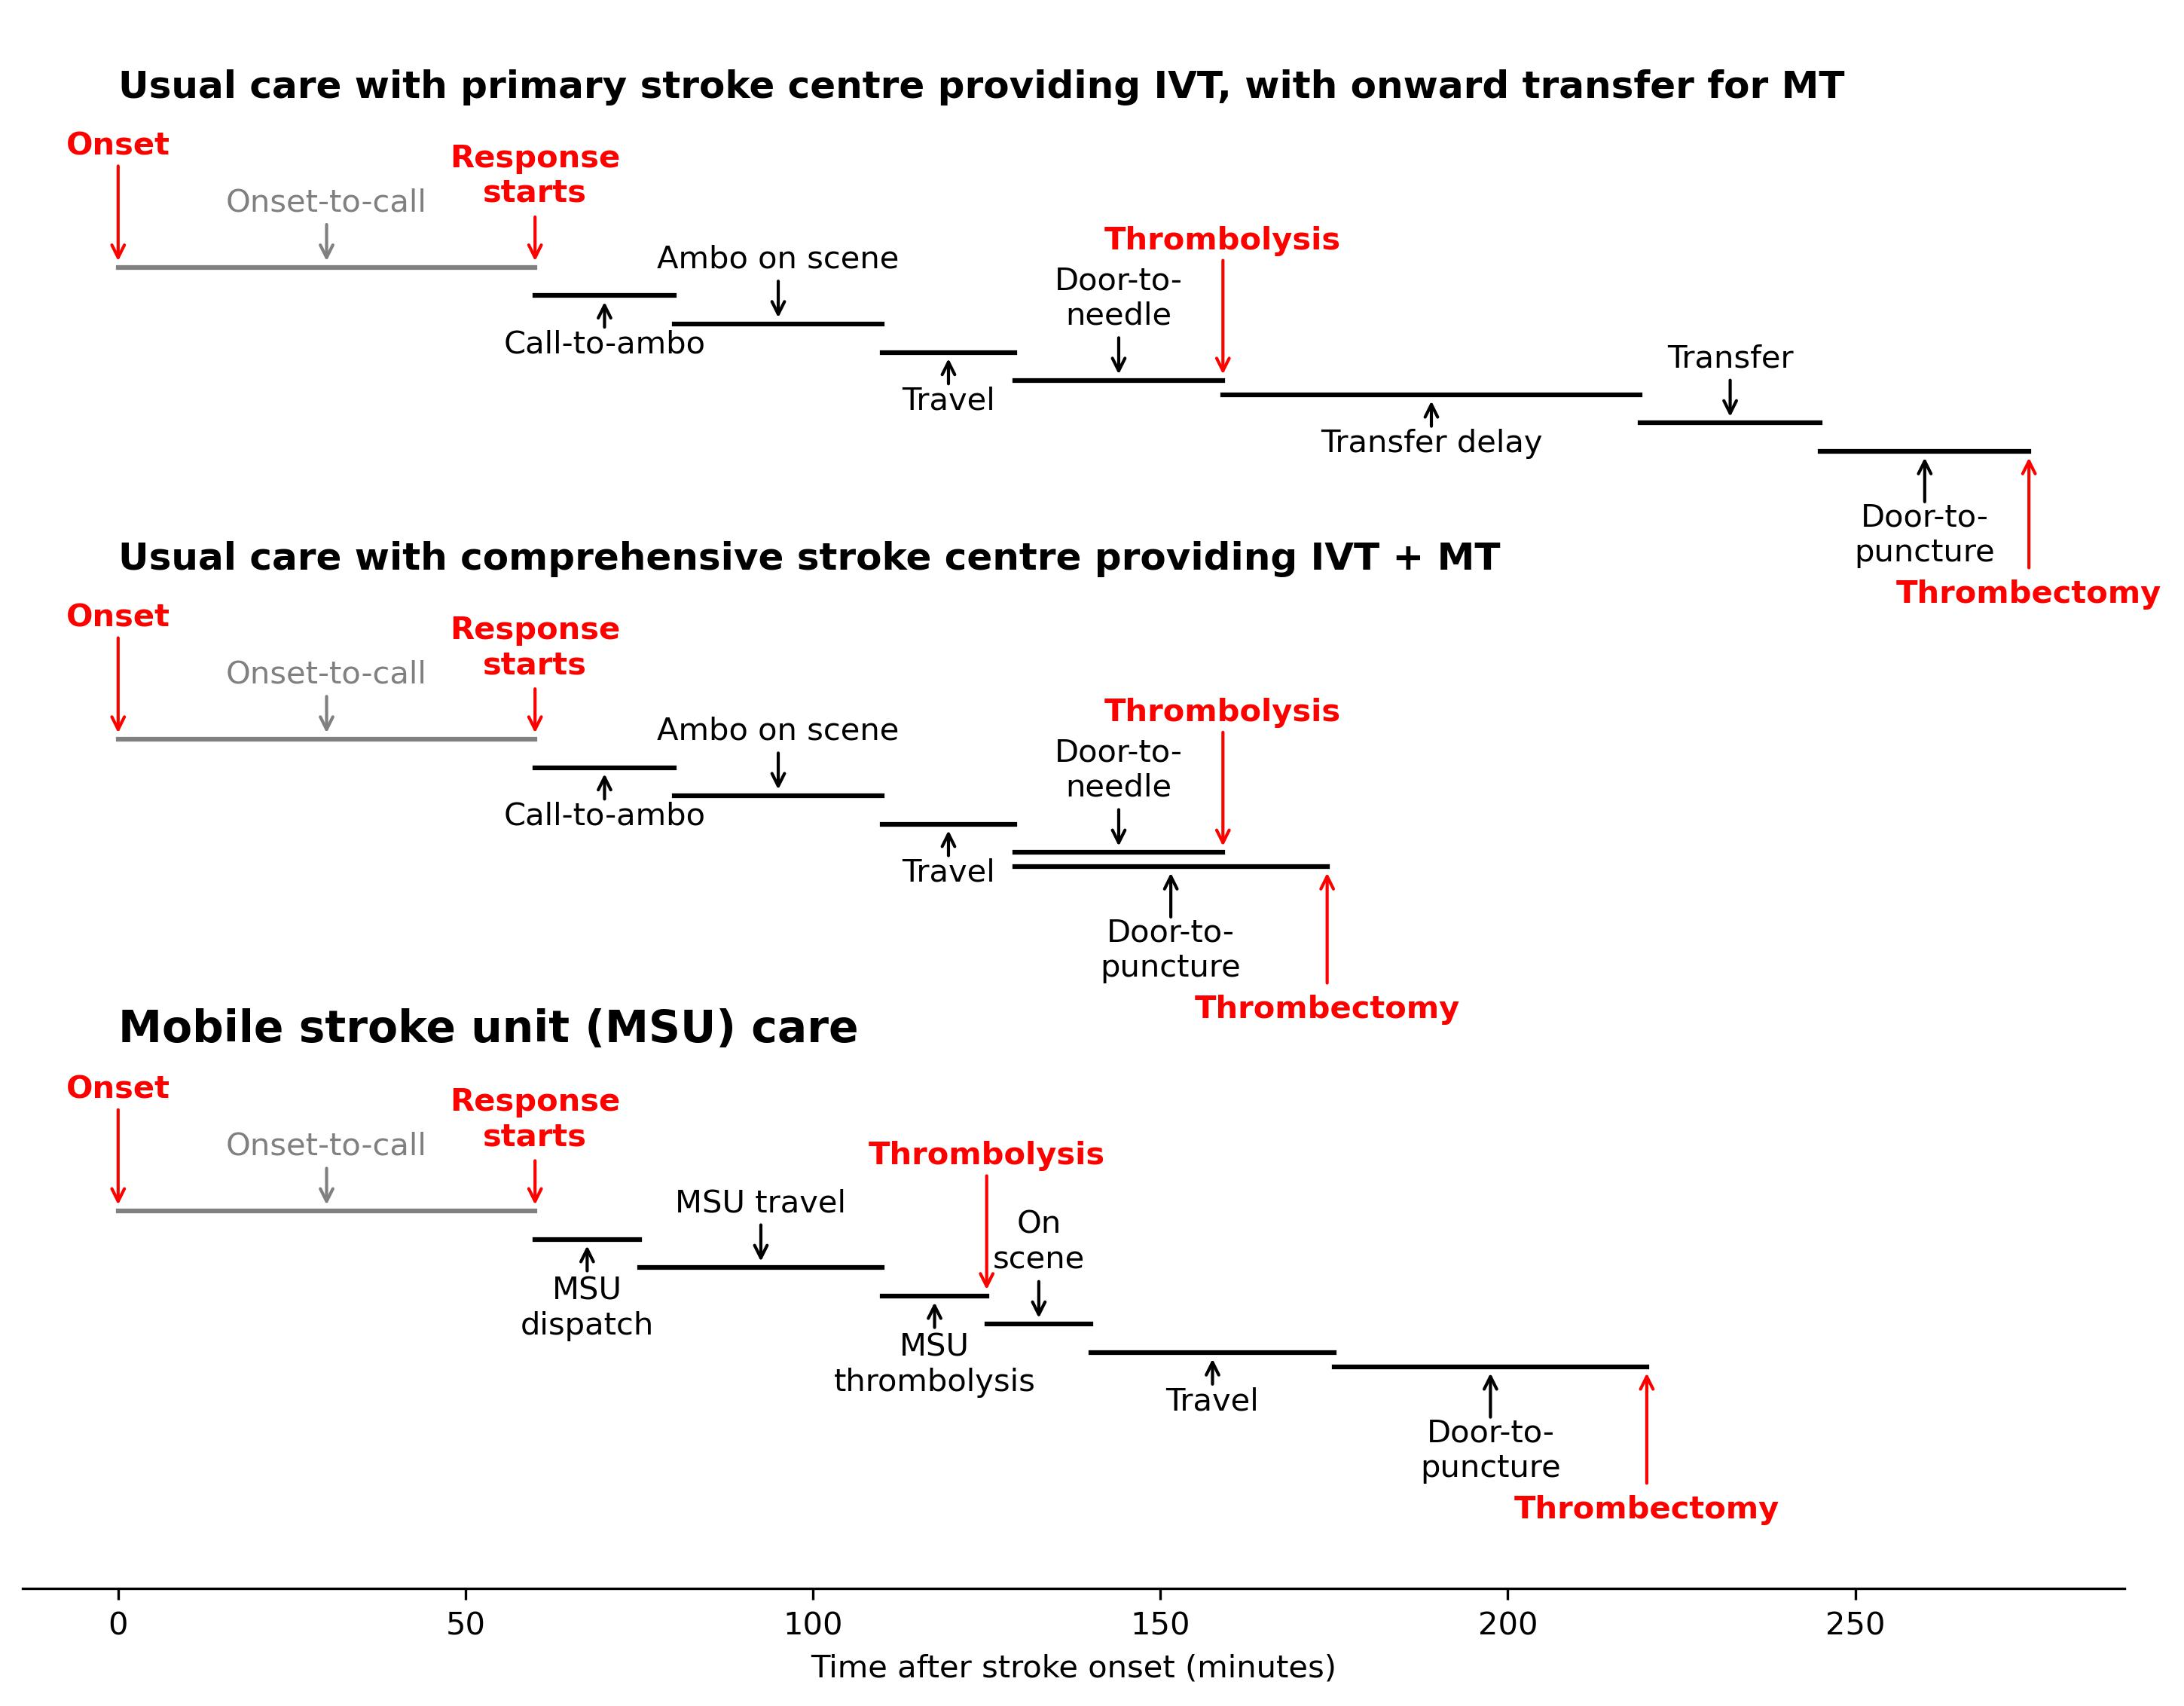
\includegraphics[width=0.85\linewidth]{images/stroke_treatment.jpg}
    \caption{An illustrative timeline showing processes included in the three pathways that are modelled for provision of IVT and MT. Top: Usual care pathway for patients with a PSC closest to their home LSOA, with the PSC providing IVT, followed by the LVO patients having a transfer to the nearest CSC for MT. Middle: Usual care pathway for patients with a CSC closest to their home LSOA, with the CSC providing both IVT and MT. Bottom: MSU care pathway, with IVT provided on-scene by the MSU, followed by the MSU transferring the LVO patients to the nearest CSC for MT. Process times other than travel times are common for all patients (defined by the scenario). Travel times depend on locations of patient and hospitals, with results calculated for all LSOAs in England.}
    \label{fig:process}
\end{figure}

For each LSOA, times to IVT and MT are calculated by summing all the non-travel process times (common for all patients and defined by the scenario) and adding required travel times (bespoke for each LSOA location, and for each inter-hospital transfer). The next section will describe how patient outcomes are calculated based on these LSOA-specific times to IVT and MT for usual care or MSU care. All calculations are performed in Python/NumPy.

\subsection{Outcome modelling}

Outcome modelling is based on published meta-analysis of clinical trials which have evaluated the decline of effectiveness  of IVT and MT over time \cite{emberson_effect_2014, fransen_time_2016}. We have applied those models to the expected real world treatment population (based on the national stroke audit of England and Wales, SSNAP). We report the expected benefit in the treated population (using a mix of nLVO and LVO derived from the patients currently arriving at hospital within 4 hours of stroke onset - as this is likely to be similar to the population where a MSU is dispatched and IVT treatment given on-scene). 

Detailed methods and code used for modelling these outcomes are available \cite{github2}, with methods described in the appendix and as an online book \cite{github3}. The outcome model is available as a PyPI package for Python \cite{pypi}.

We used modified Rankin Scale (mRS) at 3-6 months as a measure of outcome. mRS is the most commonly used instrument to describe post-stroke functional outcome \cite{quinn_functional_2009}, describing independence of living from a scale of 0 (no disability) through to 5 (severe disability requiring constant nursing attention), with death assigned an mRS of 6. A commonly used surrogate for independent living is  mRS 0-2. Health utility values for each mRS level were taken from Wang \textit{et al.} \cite{wang_utility-weighted_2020}. The mean mRS score, mean utility and proportion of patients with mRS 0-2 in a given mRS distribution can be compared between scenarios.

We calculated the patients mRS outcome distribution based on time to treatment for three patient-treatment cohorts: nLVO treated with IVT; LVO treated with IVT alone; and LVO treated with IVT and MT. For each patient-treatment cohort we calculated an mRS distribution for treatment at any given time by interpolating between the mRS distribution for treatment given at \emph{t=0} (time of stroke onset) and the mRS distribution for treatment given at \emph{t=No Effect} (time of no effect of treatment), assuming that log odds fall linearly over time \cite{emberson_effect_2014, fransen_time_2016}. Further details on how these \emph{t=0} and \emph{t=No Effect} mRS distributions were derived are given in the supplementary material.

The time to no effect was 6.3 hours for IVT \cite{emberson_effect_2014} and 8.0 hours for MT \cite{ fransen_time_2016}. Our model did not include selection of patients who may still benefit from treatment beyond these durations through the use of perfusion scanning. This number is small for IVT, but is more substantial for MT – approximately 2500 per annum in England. 

\subsection{Scenario analysis}

Scenario analysis was undertaken to investigate how changing assumed model parameters (the process durations, in minutes) affect outcomes across all LSOAs. The parameter values were varied according to the following, with all combinations modelled:

\vspace{5mm}

\begin{minipage}{1.0\textwidth}  % Define the width of the minipage
\begin{itemize}
    \item All patients:
    \begin{itemize}
        \item Stroke onset to call: 0, 60, 120, 180
    \end{itemize}
    \item Usual care:
    \begin{itemize}
        \item Call to ambulance arrival: 15, 30, 45
        \item Ambulance on-scene: 20, 30, 45
        \item Hospital arrival to IVT (door-to-needle): 30, 45
        \item Transfer-related net MT delay (excluding travel time): 30, 60, 90
        \item Hospital arrival to MT (door-to-puncture): 60, 90, 120
    \end{itemize}
    \item Mobile stroke units:
    \begin{itemize}
        \item Call to MSU dispatch: 0, 15, 30, 45
        \item MSU arrival to IVT: 15, 30, 45
        \item MSU on-scene post-IVT: 5, 15
        \item MSU hospital arrival to MT (door-to-puncture): 30, 60, 90
    \end{itemize}
\end{itemize}
\end{minipage}

\vspace{5mm}

At the CSC in the usual care pathway, the \emph{hospital arrival to MT} time has been shown to be shorter for patients transferred from a PSC, than for patients who are directly admitted \cite{hassan_impact_2022}. This is due to some of the necessary processes (such as information gathering, imaging and IVT) already being completed at the PSC. However, these patients will experience a delay in receiving MT (in addition to their inter-hospital travel time) due to waiting for transfer from the PSC. These two time durations (additional time waiting for transfer and shorter \emph{hospital arrival to MT}) are represented in the model as a single parameter: the \emph{transfer-related net MT delay} parameter. For example, if the time spent in the PSC is 90 minutes (known as the \textit{door-in-door-out} time), but the \textit{hospital arrival to MT} is reduced by 30 minutes, this is represented by setting \textit{transfer-related net MT delay} to 60 minutes in the model and leaving the \emph{hospital arrival to MT} unchanged.

\subsection{Geographic analysis}

To study geographic variation in benefit of MSU care, a single set of parameters was chosen, reflecting a reasonable base case for performance of usual care and MSU care. Process times (minutes) are shown below, with ambulance and MSU travel times and inter-hospital travel times dependent on patient location (LSOA). In this base case scenario MSUs are based at CSCs only. 

\vspace{5mm}

\begin{minipage}{1.0\textwidth}  % Define the width of the minipage
\begin{itemize}
    \item All patients:
    \begin{itemize}
        \item Stroke onset to call: 60
    \end{itemize}
    \item Usual care:
    \begin{itemize}
        \item Call to ambulance arrival: 20
        \item Ambulance on-scene: 30
        \item Hospital arrival to IVT: 45
        \item Transfer-related net MT delay (excluding travel time): 60
        \item Hospital arrival to MT: 90
    \end{itemize}
    \item Mobile stroke units:
    \begin{itemize}
        \item Call to MSU dispatch: 15
        \item MSU arrival to IVT: 30
        \item MSU on-scene post-IVT: 5
        \item MSU hospital arrival to MT: 60
    \end{itemize}
\end{itemize}
\end{minipage}

\vspace{5mm}

\subsection{Varying number of MSU base locations}

In order to study the effect of changing the number of MSU base locations, a greedy algorithm was used. In this method, 100 MSU base locations are sequentially added, with each additional one chosen from the 101 current stroke units (of any type), in the order of maximum improvement in outcomes (utility). The utility gain is calculated for those patients treated by an MSU rather than usual care; the algorithm is therefore looking at the effect of changing the number of MSU base locations, rather than the number of physical MSUs. The algorithm can also be run with MSU base locations chosen from only the 23 current CSCs.
%\section{Results}

\subsection{Scenario analysis}

Figure \ref{fig:scenarios_overview} shows the range of benefit, measured by utility or the proportion of patients with an outcome of mRS 0--2, across all of the scenarios to explore the effect of changing the process durations, with changes shown both separately for nLVO and LVO and for a combination assuming 70\% nLVO and 30\% LVO in the treated population.
For the combined nLVO/LVO population, compared with usual care, MSU care has a net improvement in:
the proportion of patients with an outcome of mRS 0--2 and a net improvement in utility for 92\% of all scenarios;
the proportion of patients with an outcome of mRS 0--2 of at least 0.01, 0.02, 0.03, or 0.04 in 77\%, 53\%, 29\%, and 11\% of all scenarios respectively;
and utility of at least 0.01, 0.02, 0.03, or 0.04 in 75\%, 49\%, 23\%, and 7\% of all scenarios respectively.
Across the majority of scenarios the benefit of MSU care over usual care was typically (interquartile range across scenarios) an improvement of the proportion of patients mRS 0--2 of 0.005 to 0.023 for nLVO, 0.017 to 0.055 for LVO treated with both IVT and MT, and 0.011 to 0.032 for the combined population. This translated to an improvement of 0.005 to 0.021 in utility for nLVO, 0.016 to 0.052 for LVO treated with both IVT and MT, and 0.010 to 0.029 for the combined population. 
The benefit to patients with LVO was derived mostly by increasing the benefit from MT due to faster treatment times after direct transport to a CSC.
% NOTE - haven't we just said the following? - 
% For the combined population there was typically (interquartile range across scenarios) an improvement of 0.010 to 0.029 in utility, and an improvement of 0.011 to 0.032 for the proportion of patients with an outcome of mRS 0--2.

\begin{figure}[h!]
    \centering
    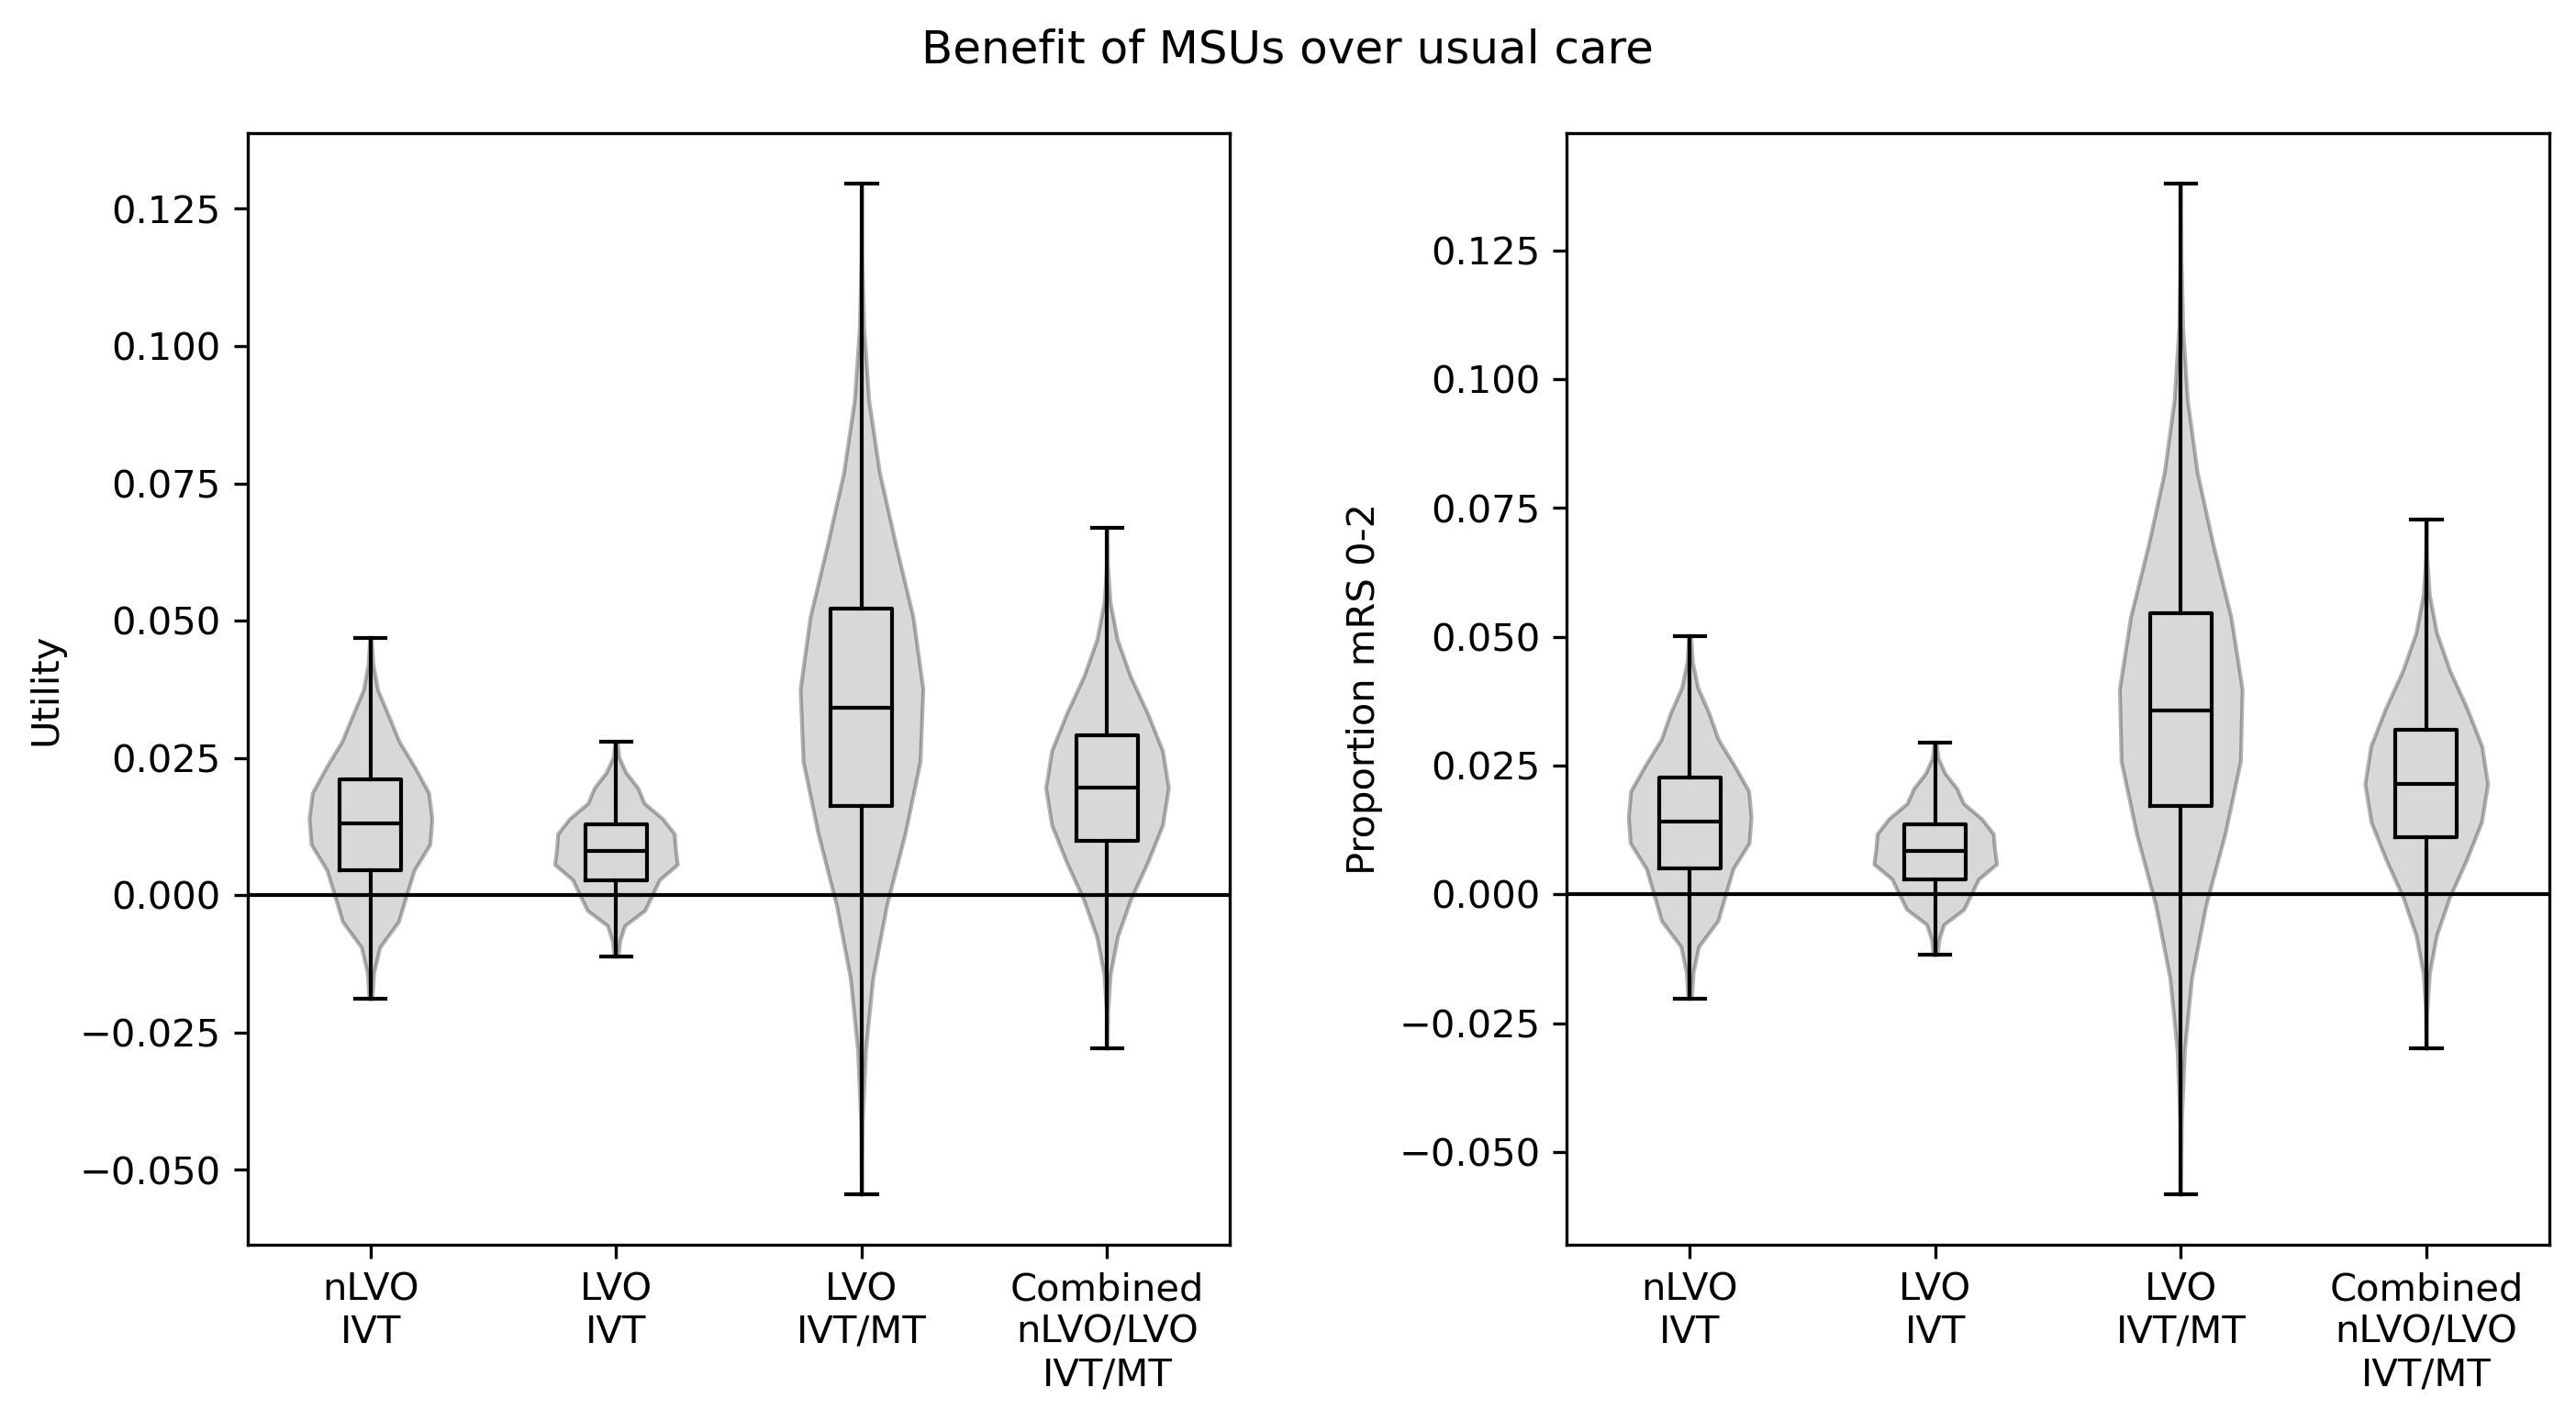
\includegraphics[width=0.75\linewidth]{images/scenario_results_summary.png}
    \caption{Benefit of MSU care over usual care across all scenarios (exploring the effect of changing process durations), in the treated population, measured by utility (left) or the proportion of patients with an outcome of mRS 0--2 (right), separating the changes for patients with nLVO and LVO. Results for LVO patients show the effect of MSU care on the benefit derived from IVT alone, or by IVT/MT in combination. Box plots show range, interquartile range, and median across all scenarios. The combined nLVO/LVO benefit assumed 70\% nLVO and 30\% LVO in the treated population, with LVOs receiving IVT/MT in combination. Overlaid on the box plots are violin plots showing the distribution of results across all scenarios. A positive value indicates MSU care provides an advantage over usual care, and a negative value indicates MSU care is disadvantageous compared with usual care. Results are the average effect across all LSOAs in England.}
    \label{fig:scenarios_overview}
\end{figure}

Figures \ref{fig:scenarios_mrs}  and \ref{fig:scenarios_utility} show how changing modelled process durations affects the predicted benefit of MSU care, expressed in proportion of patients with an outcome of mRS 0--2 or utility, respectively. Results show the combined effect on nLVO/LVO, with patients with LVO receiving IVT/MT in combination. Changing time from onset to call only had marginal effect on the benefit of MSU care over usual care. Changing parameters that worsen usual care (such as lengthening ambulance response times, or lengthening arrival to IVT), lead to increased advantages of MSU care over usual care. Likewise, changing parameters that improve MSU care (such as MSU dispatch times, or time to IVT on scene) increased the advantages of MSU care over usual care.

\begin{figure}[h!]
    \centering
    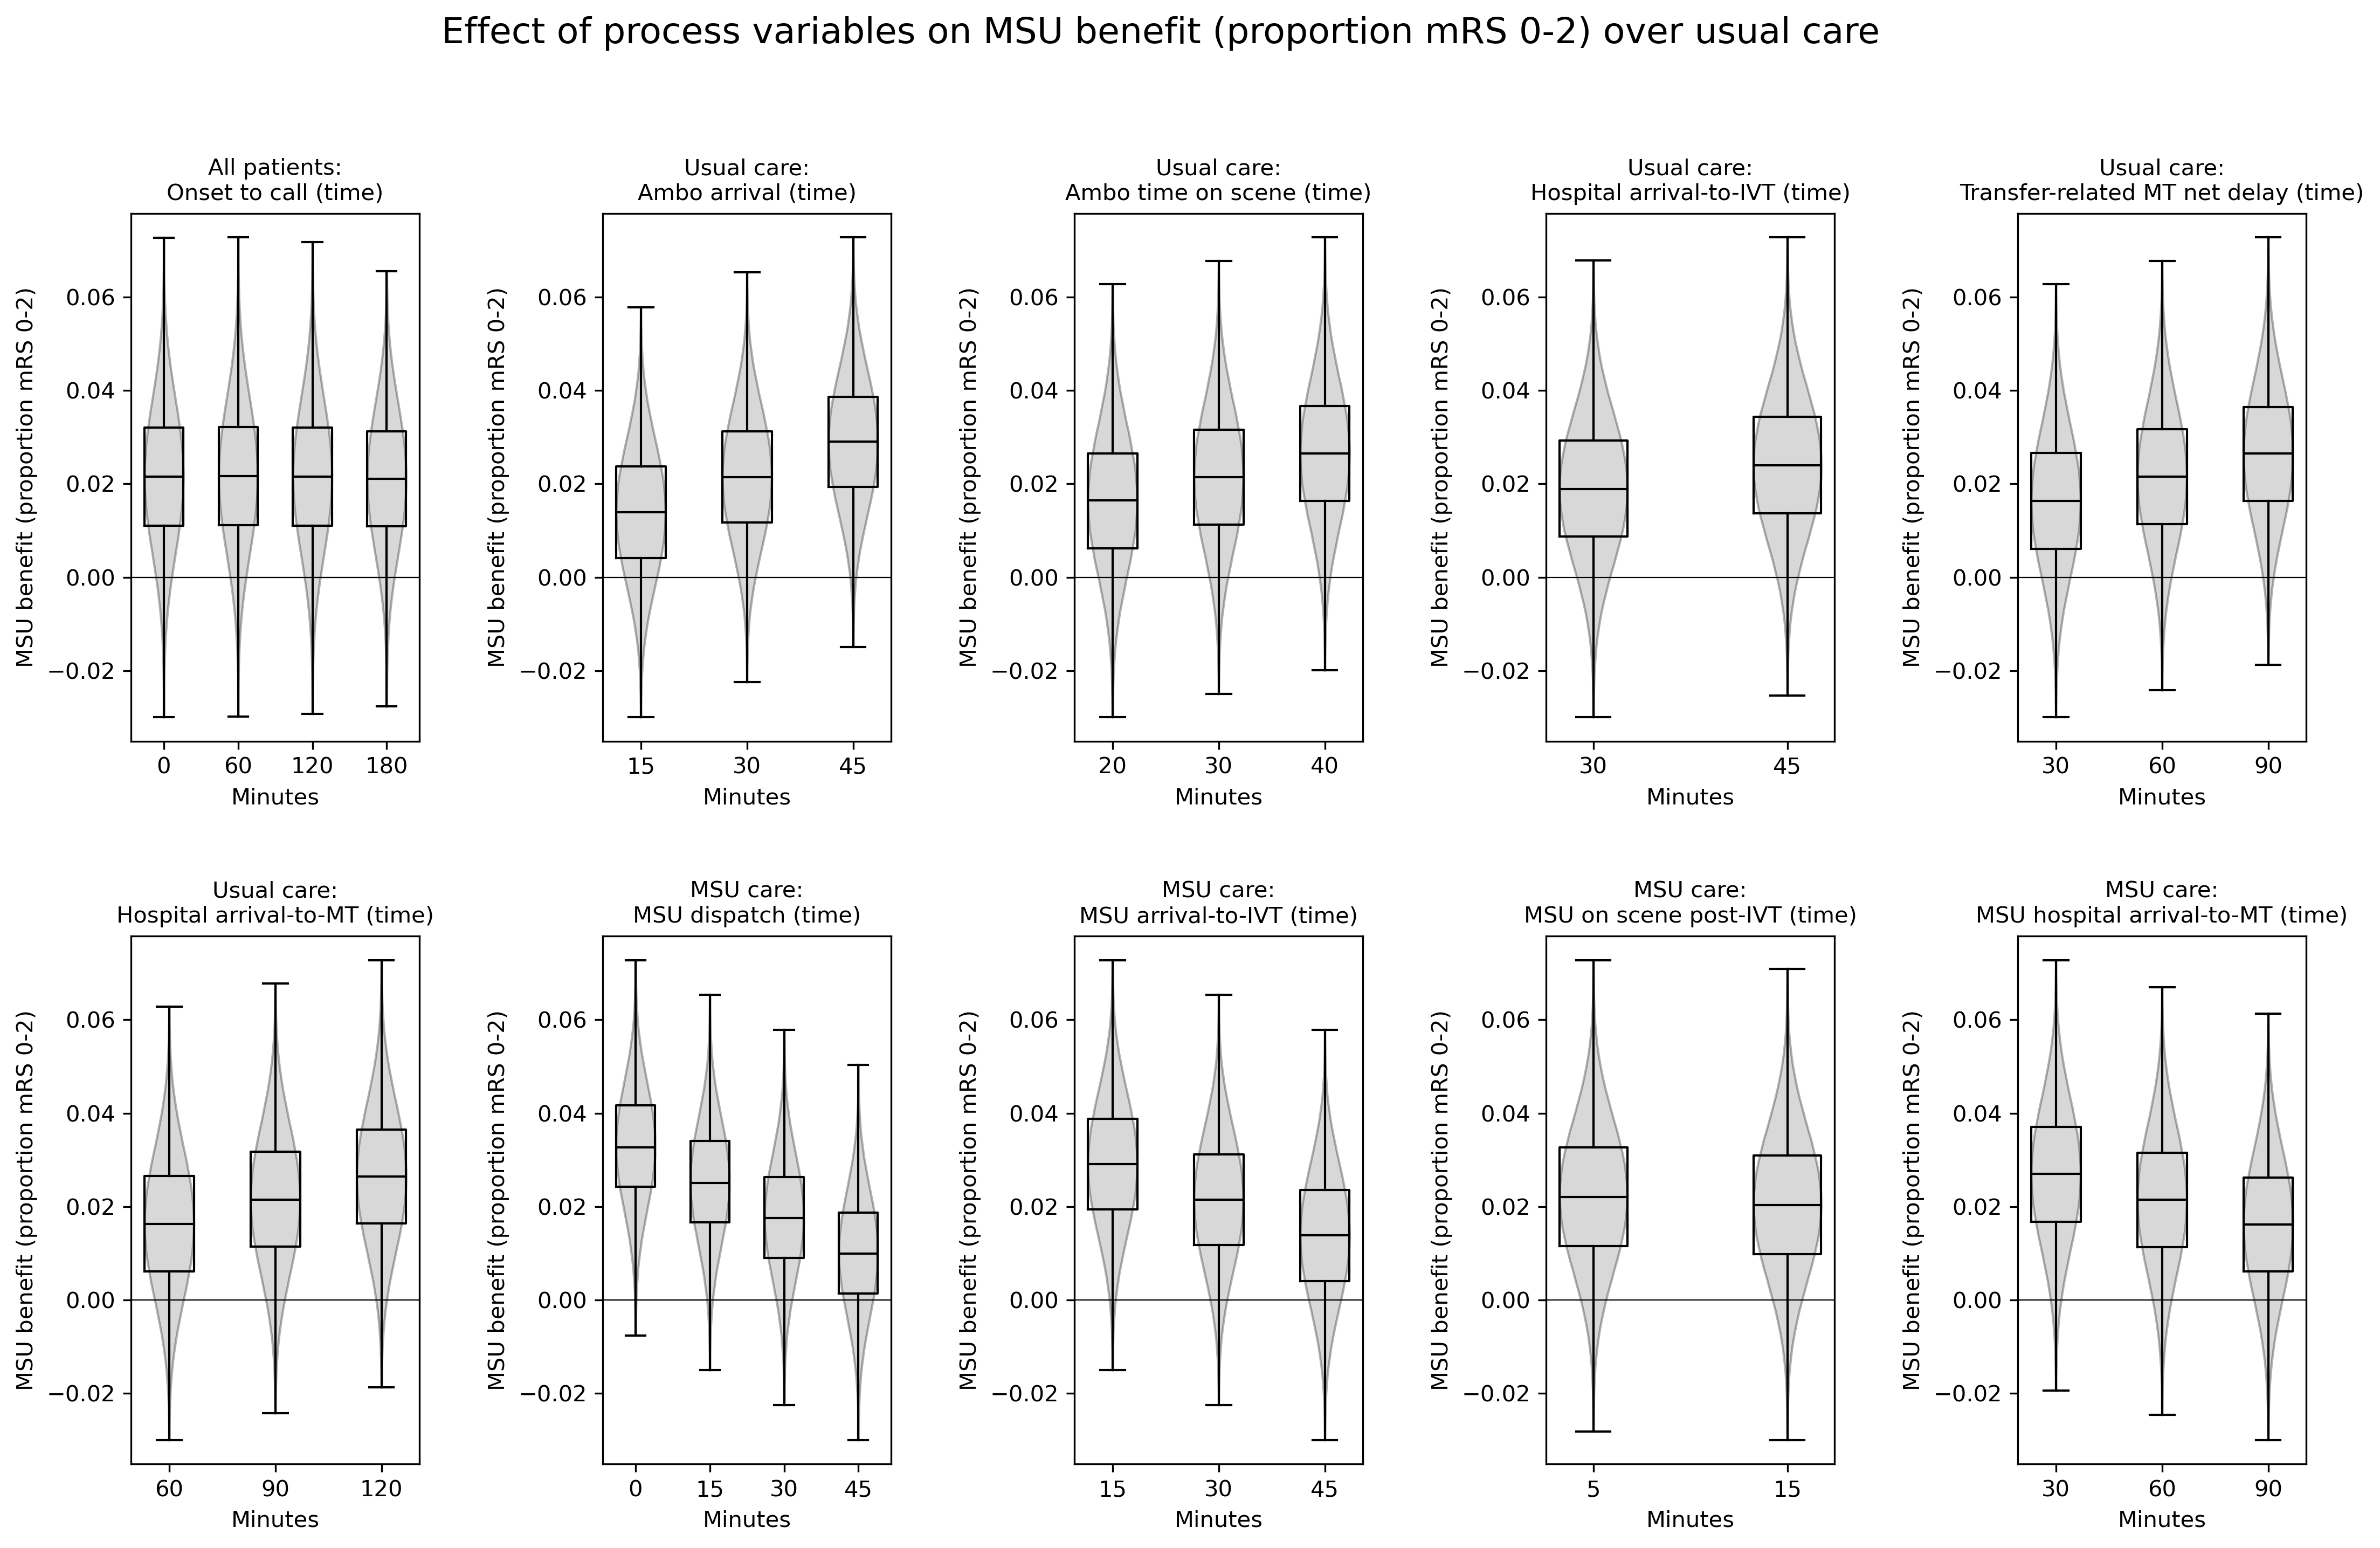
\includegraphics[width=1\linewidth]{images/msu_net_mrs_0-2_benefit.png}
    \caption{The effect of changing modelled process durations on the predicted benefit of MSU care over usual care, in the treated population (comprised of 70\% nLVO and 30\% LVO patients, where nLVO patients receive IVT and LVO patients receive IVT followed by MT), measured by proportion of patients with an outcome of mRS 0--2. For each target parameter, results are averaged across all scenarios with that given parameter value. Box plots show range, interquartile range, and median, across all scenarios. Overlaid over the box plots are violin plots showing the distribution of results across all scenarios. Results are the average effect across all LSOAs in England.}
    \label{fig:scenarios_mrs}
\end{figure}

\begin{figure}[h!]
    \centering
    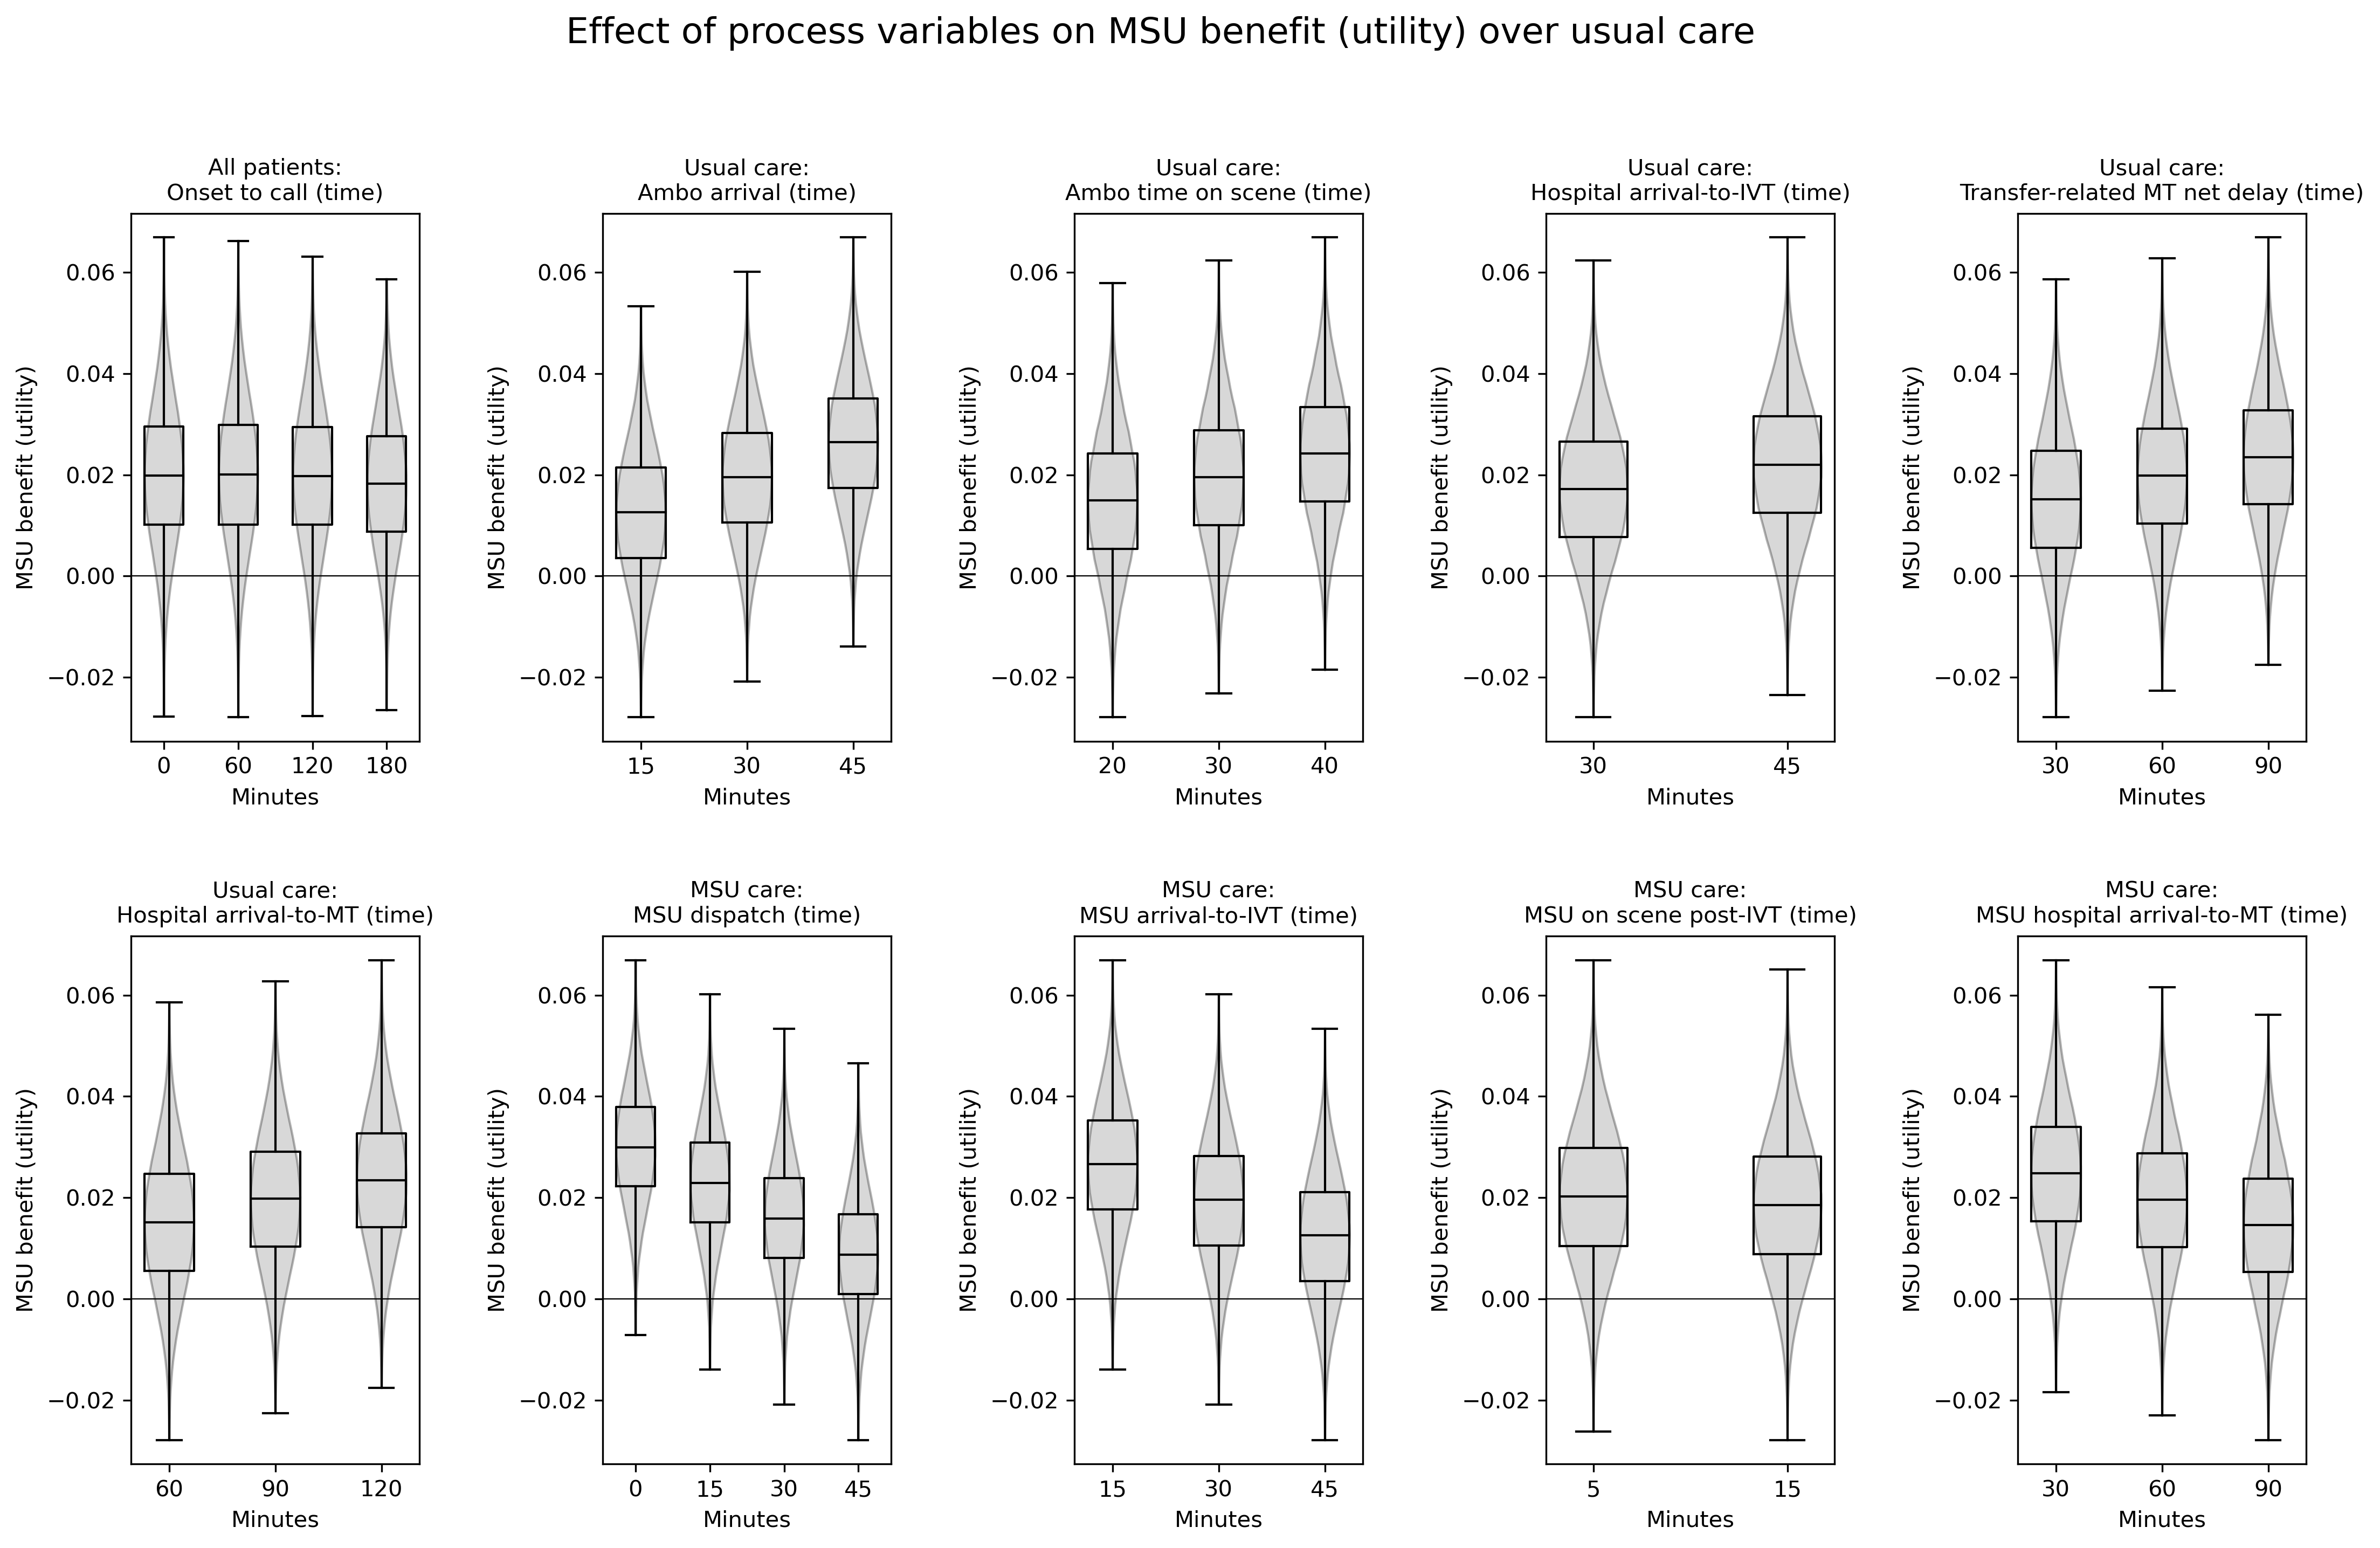
\includegraphics[width=1\linewidth]{images/msu_net_utility_benefit.png}
    \caption{The effect of changing modelled process durations on the predicted benefit of MSU care over usual care, in the treated population (comprised of 70\% nLVO and 30\% LVO patients, where nLVO patients receive IVT and LVO patients receive IVT followed by MT), measured by utility. For each target parameter, results are averaged across all scenarios with that given parameter value. Box plots show range, interquartile range, and median, across all scenarios. Overlaid over the box plots are violin plots showing the distribution of results across all scenarios. Results are the average effect across all LSOAs in England.}
    \label{fig:scenarios_utility}
\end{figure}

\subsection{Geographic variation}

For this comparison, the MSUs are based at CSCs only and we assume there is a mix of 70\% nLVO and 30\% LVO in the treated population in which nLVO patients receive IVT and LVO patients receive IVT followed by MT.

Figure \ref{fig:map_times} shows travel and transfer times for usual care and for MSU care. Under usual care, when a patient first attends a PSC (providing only IVT), the travel/transfer time to MT include the travel time to the nearest PSC, and a net additional 60 minute delay (taking into account the \textit{door-in-door-out} time at the first admitting hospital and a reduction in time to MT at the CSC for transferred patients). Under usual care, there is significant variation in travel times from patient LSOA to the first attended centre (PSC or CSC) for IVT, but there is more substantial variation in times to MT due to some patients (67\% of LSOAs and 70\% of admissions) requiring a transfer for MT. Under MSU care, as the MSUs are based at CSCs only, travel times for an MSU to deliver IVT can exceed the travel time of a normal ambulance to the closest centre providing IVT, and this extra travel time can lead to delayed time to IVT in those LSOAs furthest away from MSU base locations. However, for patients living in LSOAs that are close to a CSC, but with a PSC even closer, these patients benefit from MT sooner under MSU care than compared to usual care as they avoid the delays relating to attending the PSC first.

\begin{figure}[h!]
    \centering
    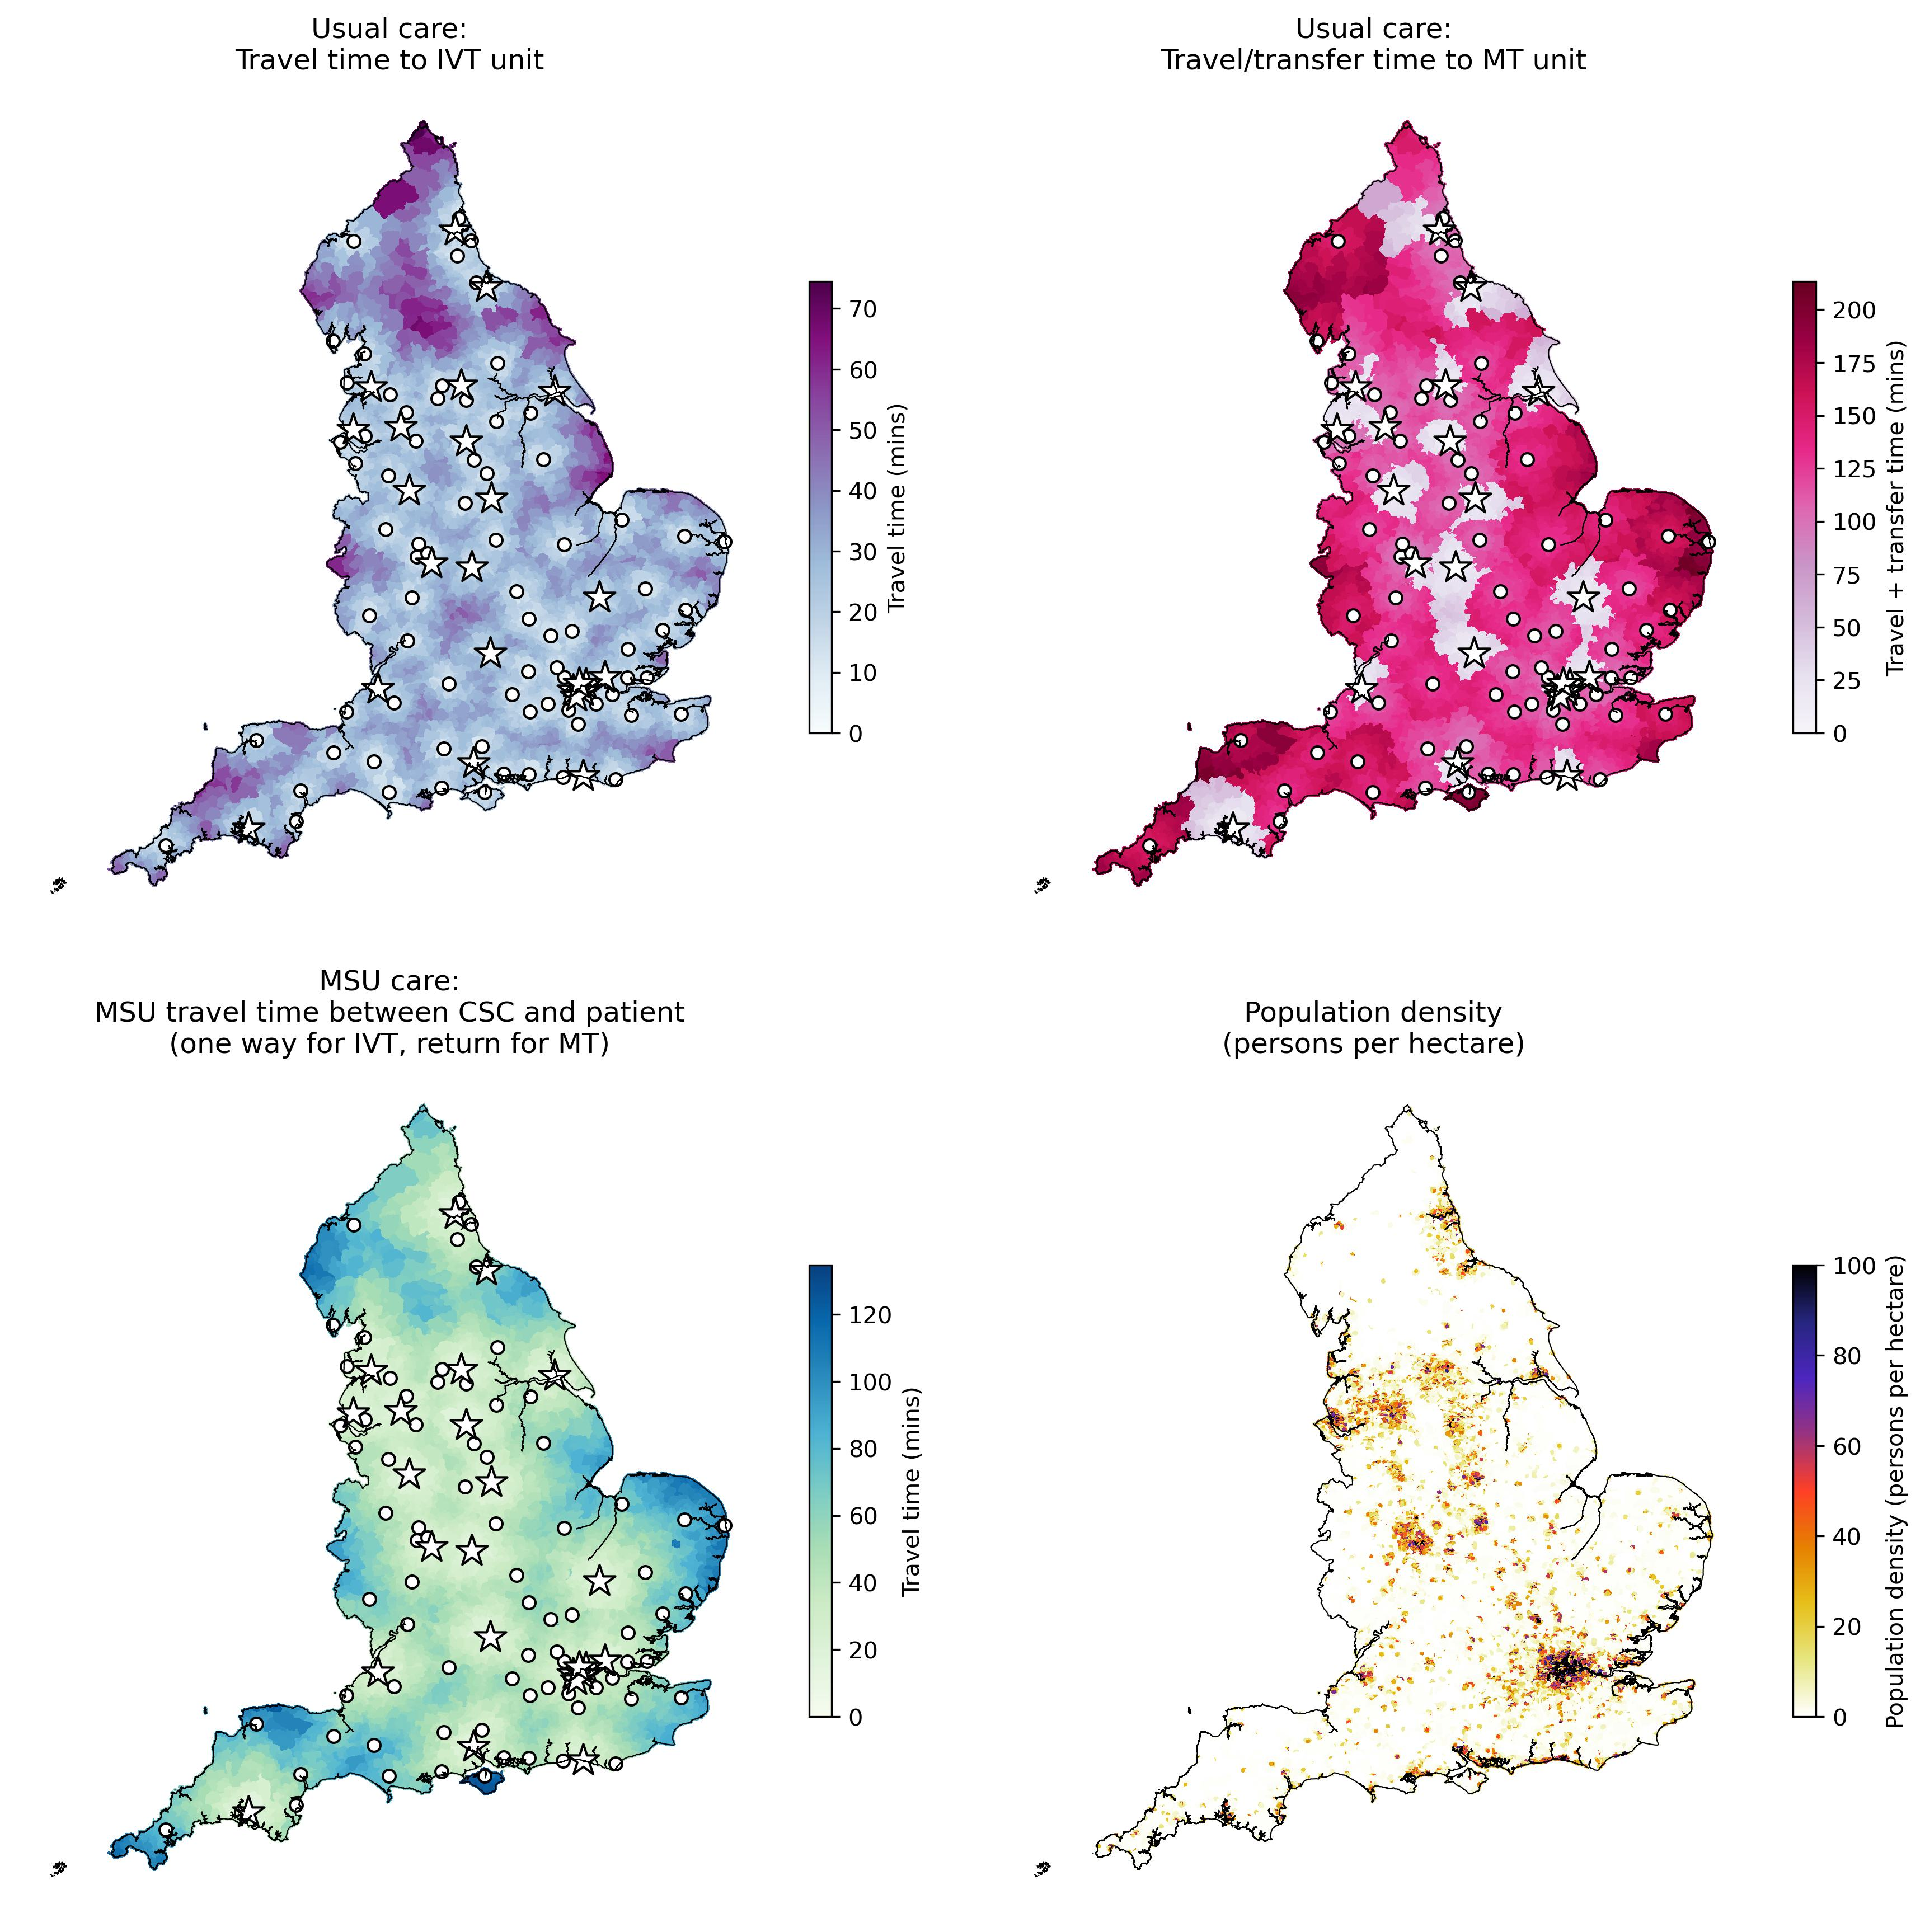
\includegraphics[width=1.0\linewidth]{images/map_times.jpg}
    \caption{Travel times to treatment under the two treatment delivery models, and population density for each LSOA. \textit{Top left}: With \emph{usual care} the travel times from the patients LSOA to their nearest PSC (providing only IVT). \textit{Top right}: With \emph{usual care} the travel and, where necessary, transfer times from the patients LSOA to a CSC (providing MT). For those patients that first attend a PSC providing only IVT, the times shown include the travel time to the PSC, a net additional delay of 60 minutes, and the inter-hospital travel time between PSC and CSC. \textit{Bottom left}: With \emph{MSU care} with the MSU base locations at the current 23 CSCs, the travel times for the MSU between the patients LSOA and their nearest CSC (one way for travel time to IVT, return journey for travel time to MT). \textit{Bottom right}: Population density (with scale capped at 100 persons per hectare). Circles show locations of PSCs (providing only IVT). Stars show locations of CSCs (providing both IVT and MT), and being the base locations of MSUs.}
    \label{fig:map_times}
\end{figure}

Figures \ref{fig:msu_map_mrs_0_2} and \ref{fig:msu_map_utility} show maps (by ischaemic stroke subtype) of geographic variation in benefit (expressed in proportion of patients with an outcome of mRS 0--2 or utility, respectively) between treatment delivery models. Overall, with no reperfusion treatment, there is an average outcome utility of 0.52 across the combined population. With usual care, there is a utility gain of 0.086 in treated patients. MSU care provided an average further utility gain in treated patients of 0.022 over usual care. There is significant variation in the benefit of reperfusion using usual care, with those living closest to CSCs receiving the greatest benefit. This is due to the larger utility gain of reperfusion treatment coming from the treatment of LVO, and with those patients benefiting most from rapid access to MT.

The benefit of MSU care over usual care follows different patterns for nLVO and LVO patients. For nLVO patients, the benefit of MSU care decreases with increased distance from the MSU base location. For LVO patients the benefit of MSU care first decreases with increased distance from the MSU base location, but then benefit increases where use of the MSU avoids inter-hospital transfer for MT, before decreasing again with greater travel times for the MSU. The catchment area of benefit for LVO under MSU care is therefore wider than the catchment area of benefit for nLVO, with the maximum benefit being in a halo a little distance from the MSU base location, where patient transfer for MT is avoided but MSU travel times are still acceptable.

\begin{figure}[h!]
    \centering
    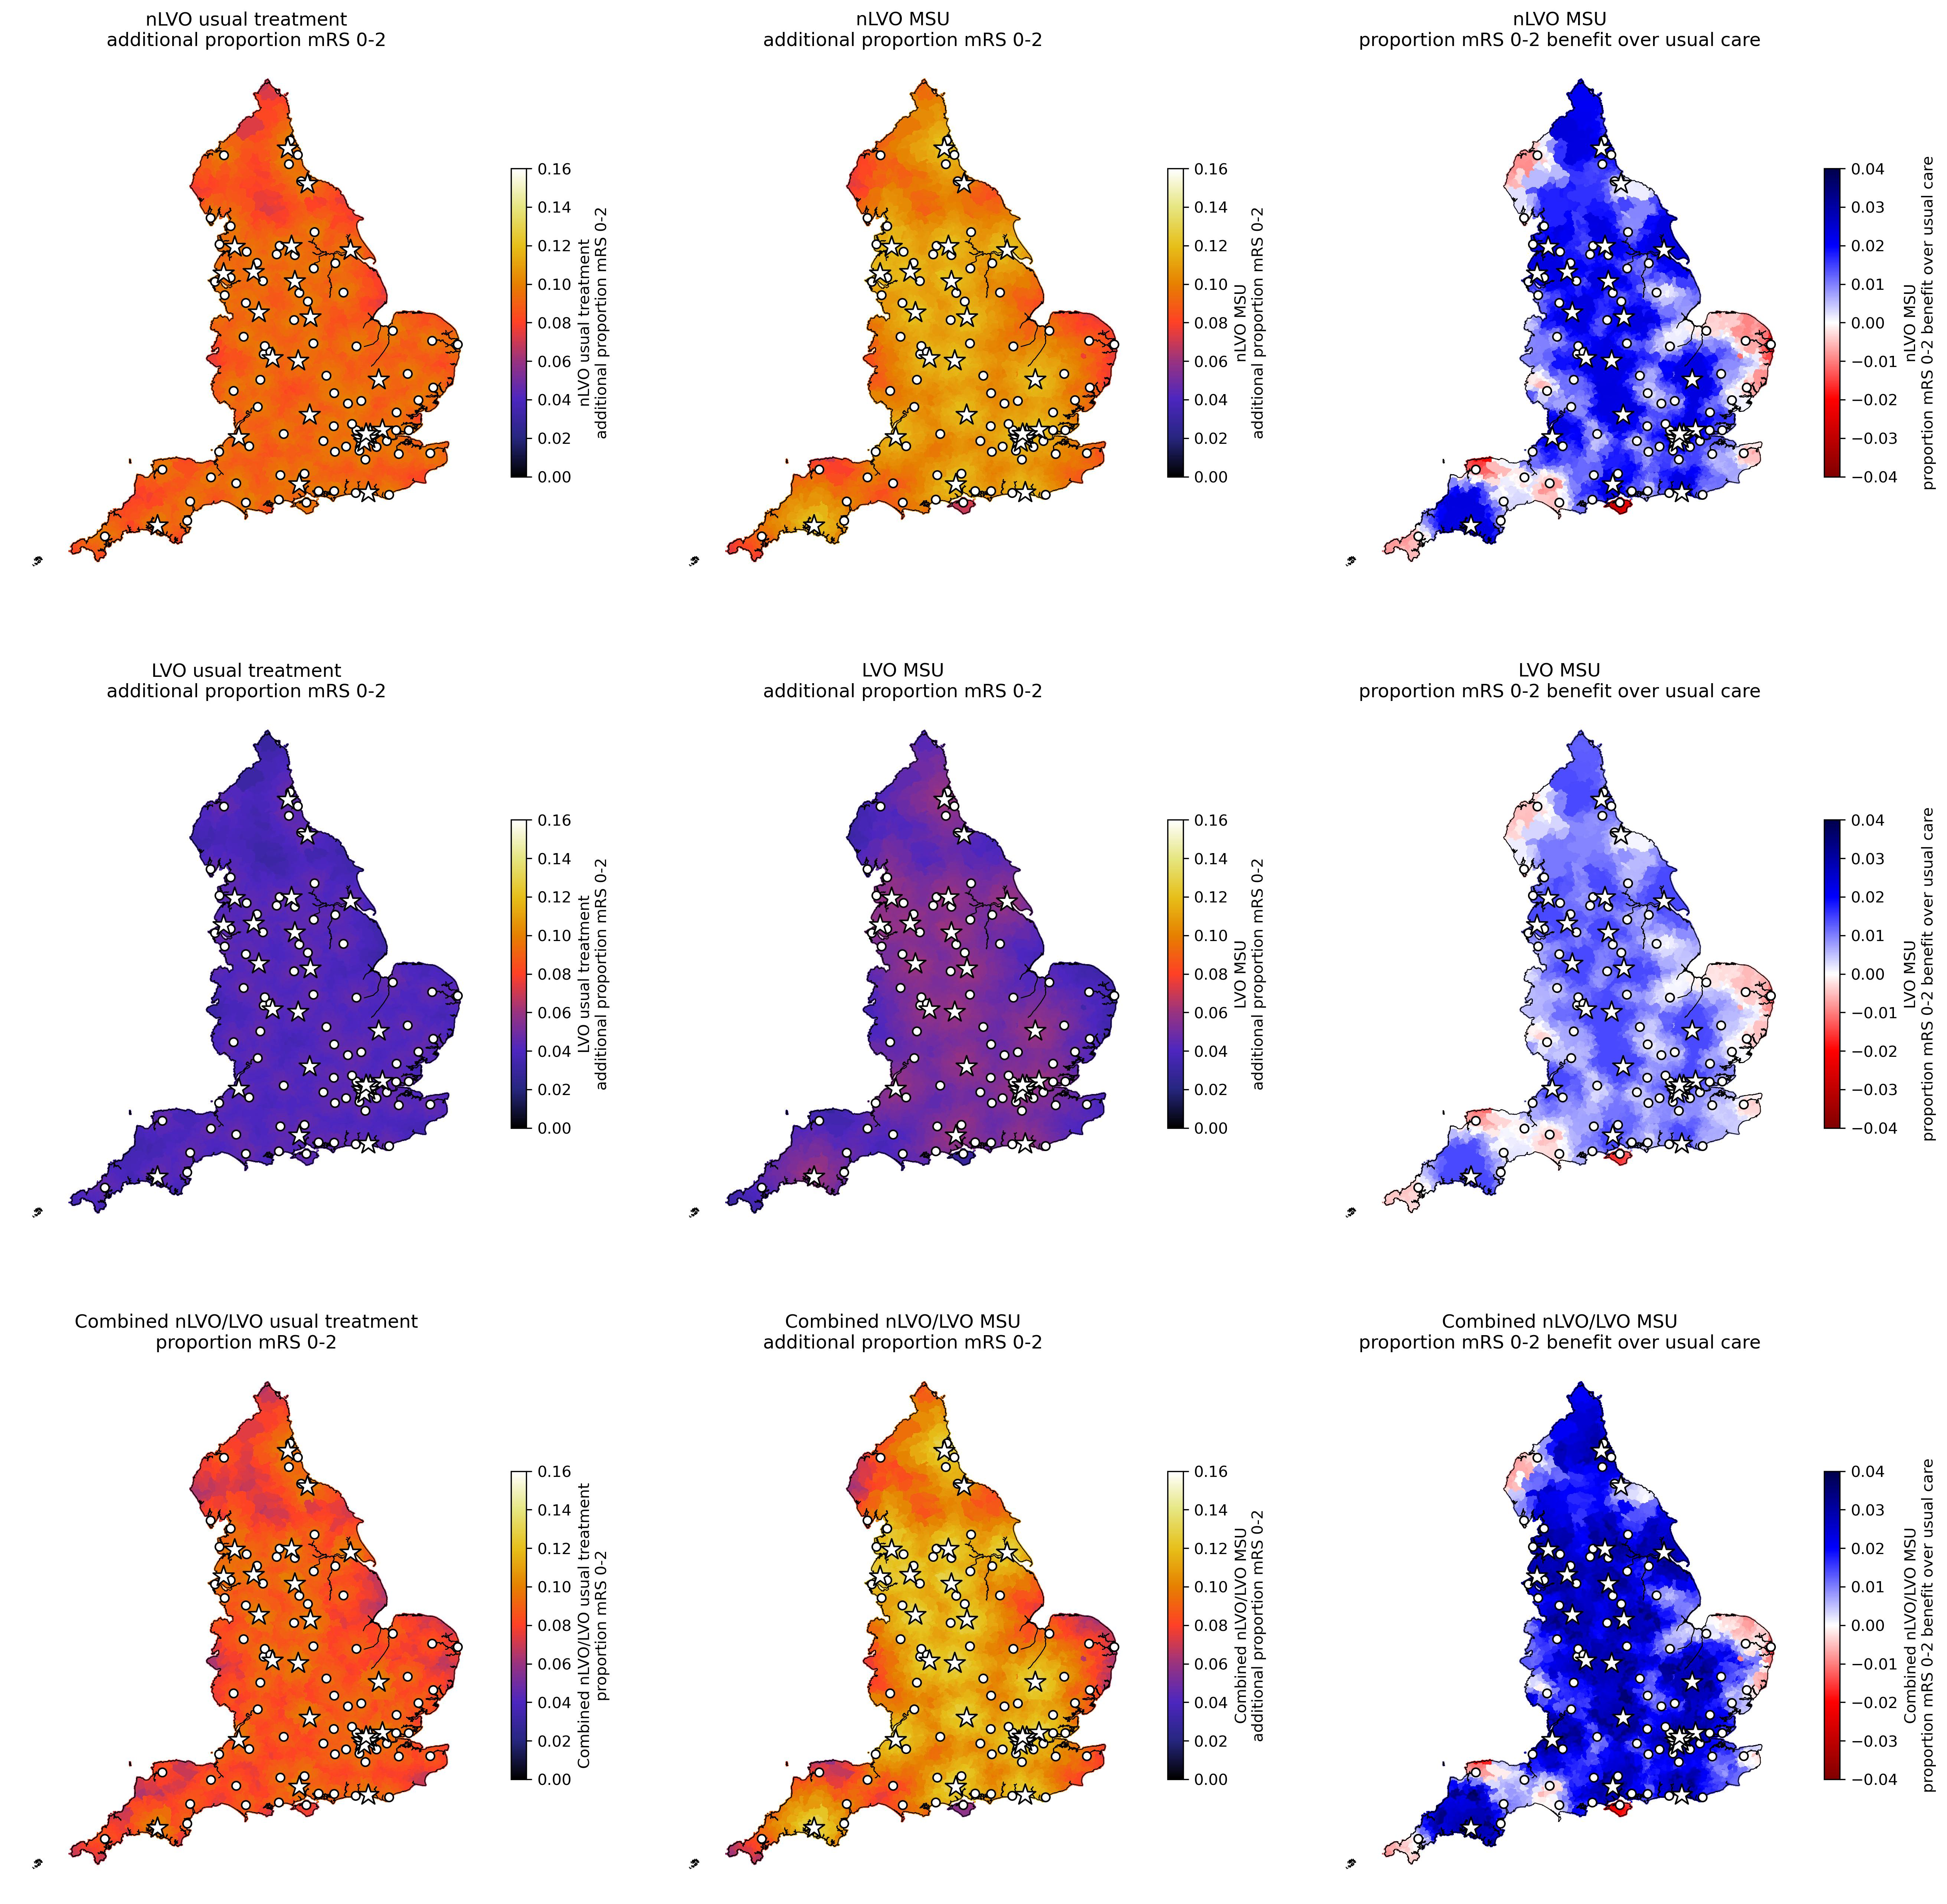
\includegraphics[width=1\linewidth]{images/map_mrs_0_2.jpg}
    \caption{Map of treatment benefits expressed as the proportion of patients with an outcome of mRS 0--2, calculated by LSOA for the treated population. \textit{Top}: Treatment of nLVO; \textit{Middle}: Treatment of LVO, \textit{Bottom}: Combination of treatment (based on 70\% nLVO and 30\% LVO in the treated population, with LVO receiving IVT/MT in combination). \textit{Left}: Benefit of usual care over no treatment; \textit{Middle}: Benefit of MSU care over no treatment; \textit{Right}: Benefit of MSU care over usual care. Circles show locations of PSCs (providing only IVT). Stars show locations of CSCs (providing both IVT and MT, and are also the base locations of MSUs).}
    \label{fig:msu_map_mrs_0_2}
\end{figure}

\begin{figure}[h!]
    \centering
    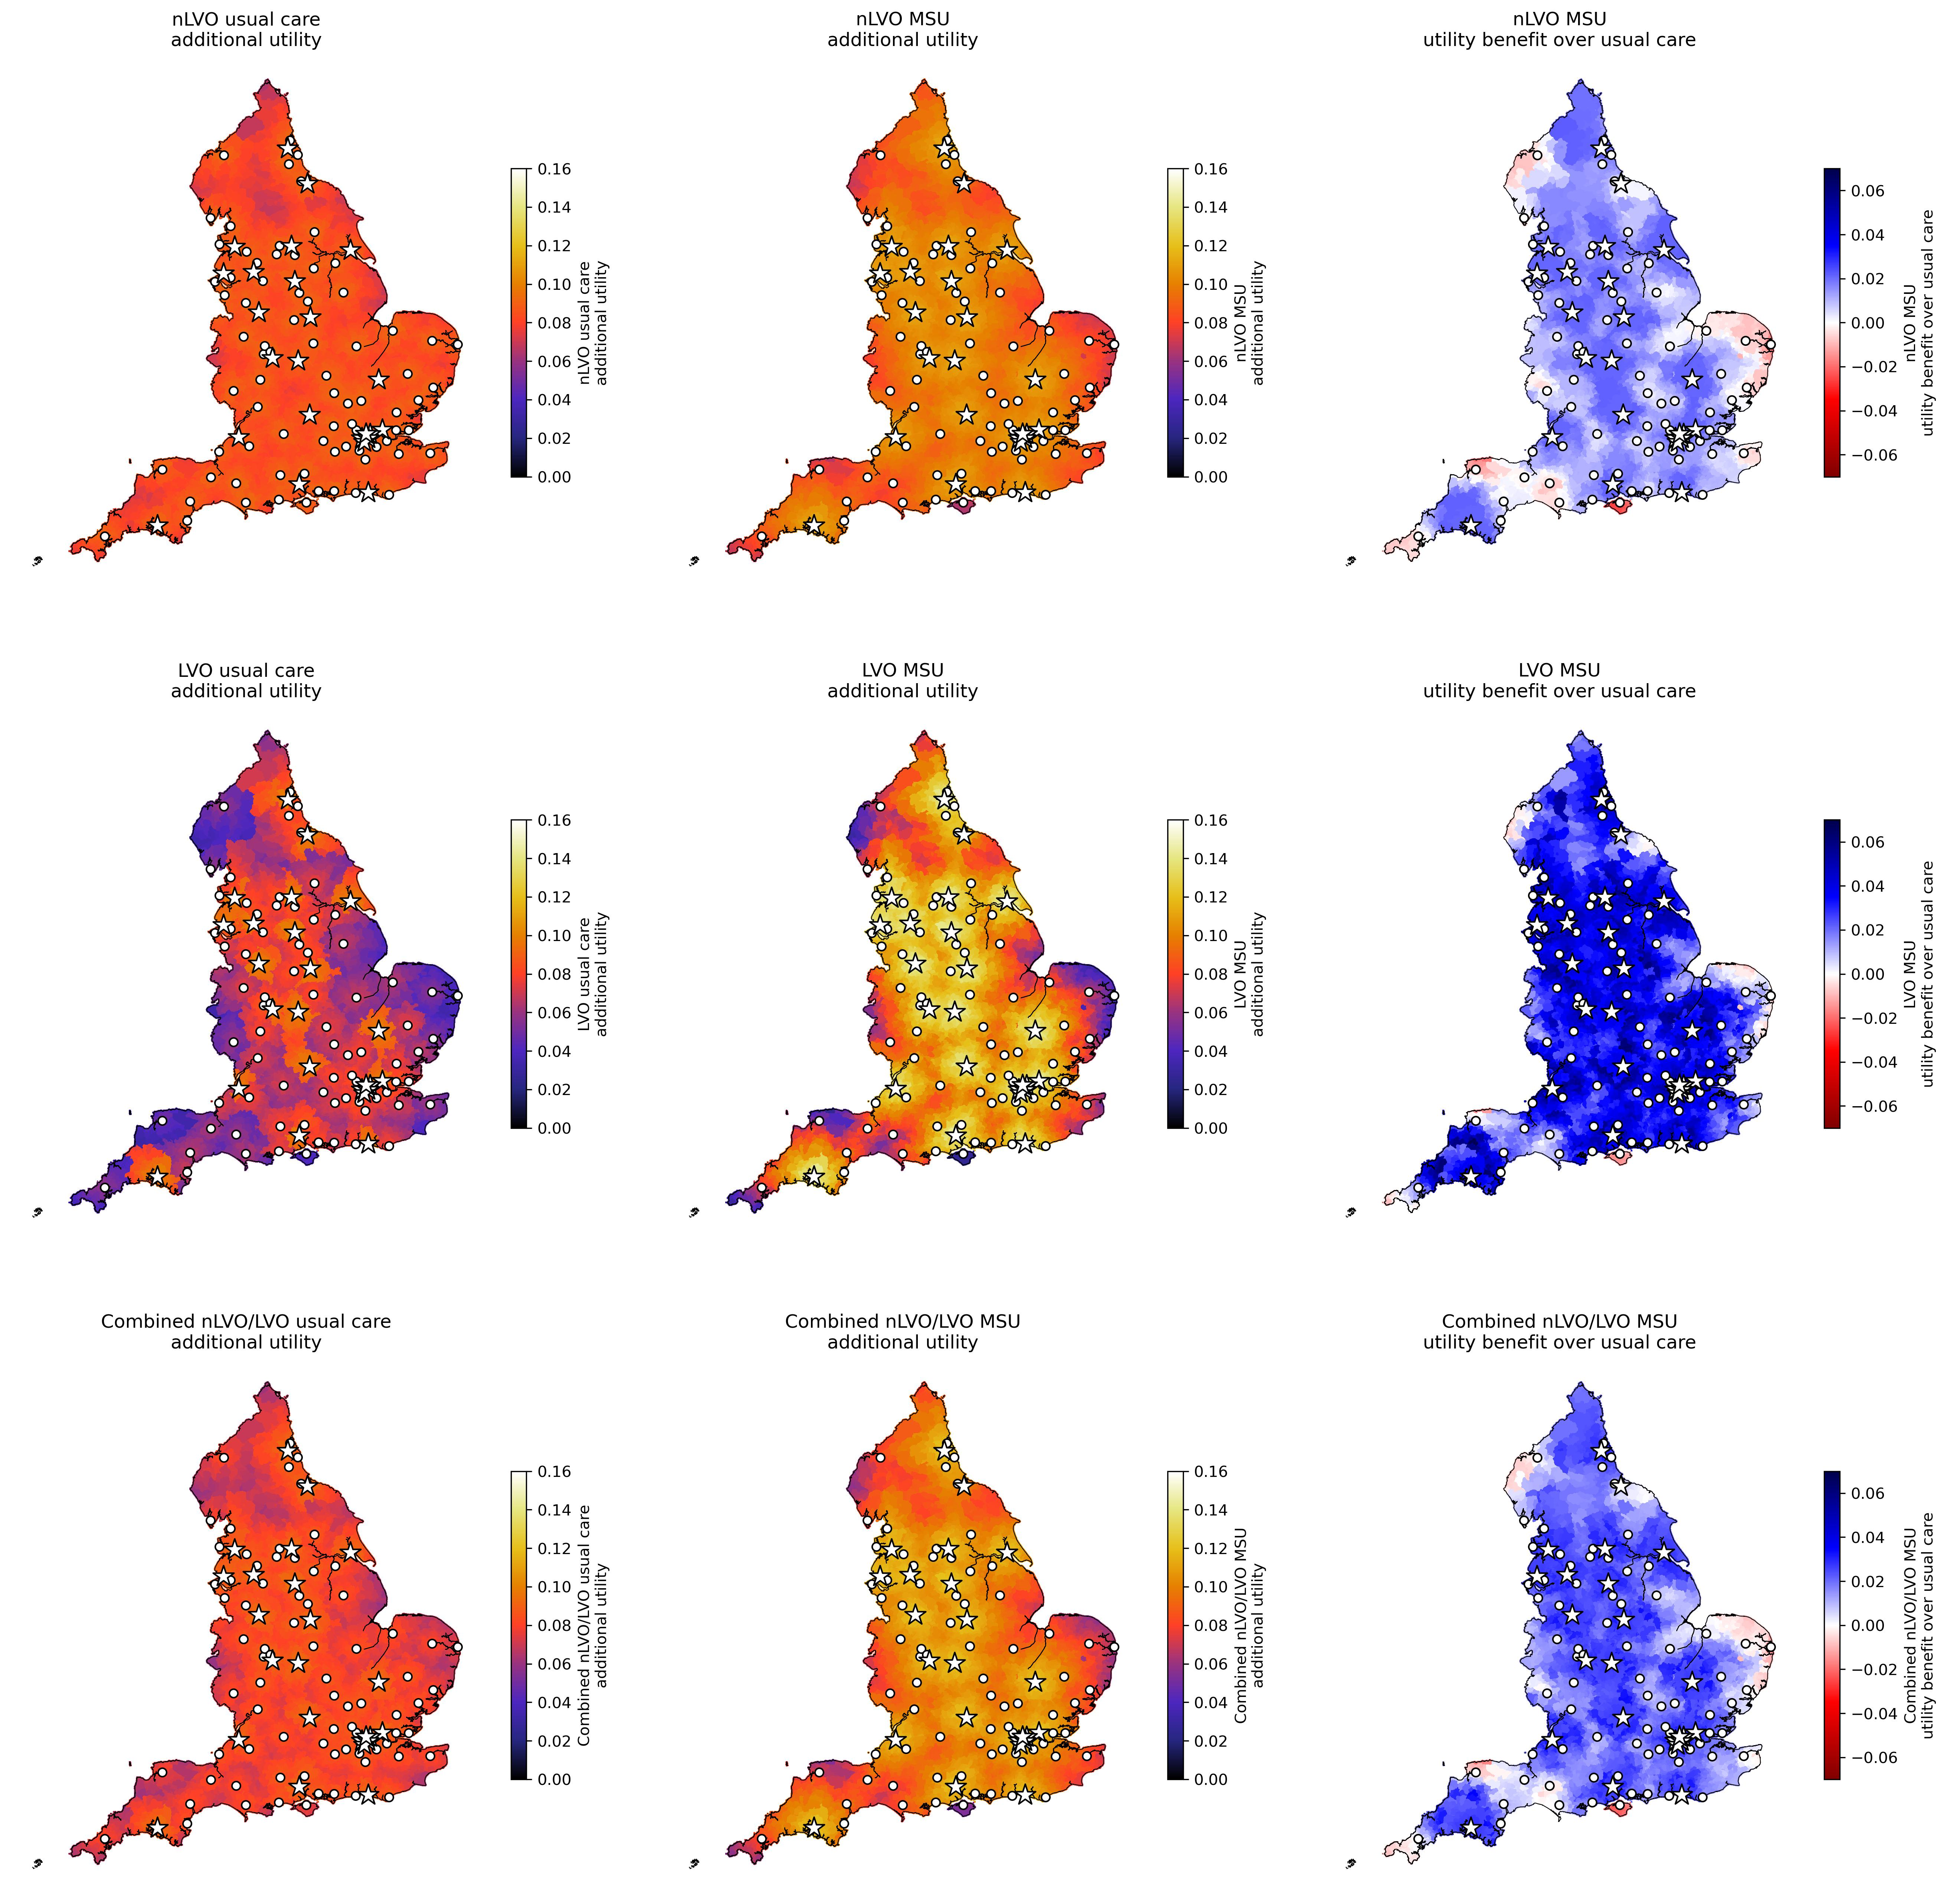
\includegraphics[width=1\linewidth]{images/map_utility.jpg}
    \caption{Map of treatment benefits expressed as the  utility benefit, calculated by LSOA for the treated population. \textit{Top}: Treatment of nLVO; \textit{Middle}: Treatment of LVO, \textit{Bottom}: Combination of treatment (based on 70\% nLVO and 30\% LVO in the treated population, with LVO receiving IVT/MT in combination). \textit{Left}: Benefit of usual care over no treatment; \textit{Middle}: Benefit of MSU care over no treatment; \textit{Right}: Benefit of MSU care over usual care. Circles show locations of PSCs (providing only IVT). Stars show locations of CSCs (providing both IVT and MT, and are also the base locations of MSUs).}
    \label{fig:msu_map_utility}
\end{figure}


Figure \ref{fig:msu_histograms} shows histograms of benefit of MSU care over usual care for the modelled population, with benefit represented as time to treatment, proportion of patients with outcome mRS 0--2 after stroke, and utility. For most LSOAs MSU care improves the time to IVT and MT, but some areas have worsened times. This is reflected in most areas having a benefit of about a 0.03 increase in the proportion of patients with mRS 0--2 after stroke, and similarly a benefit of about a 0.03 increase in utility after stroke. Some areas though have reduced benefit, or even disbenefit of using MSUs. The maximum benefit is about 0.04 improvement in both the proportion of patients with mRS 0--2 after stroke and utility after stroke.

\begin{figure}[h]
    \centering
    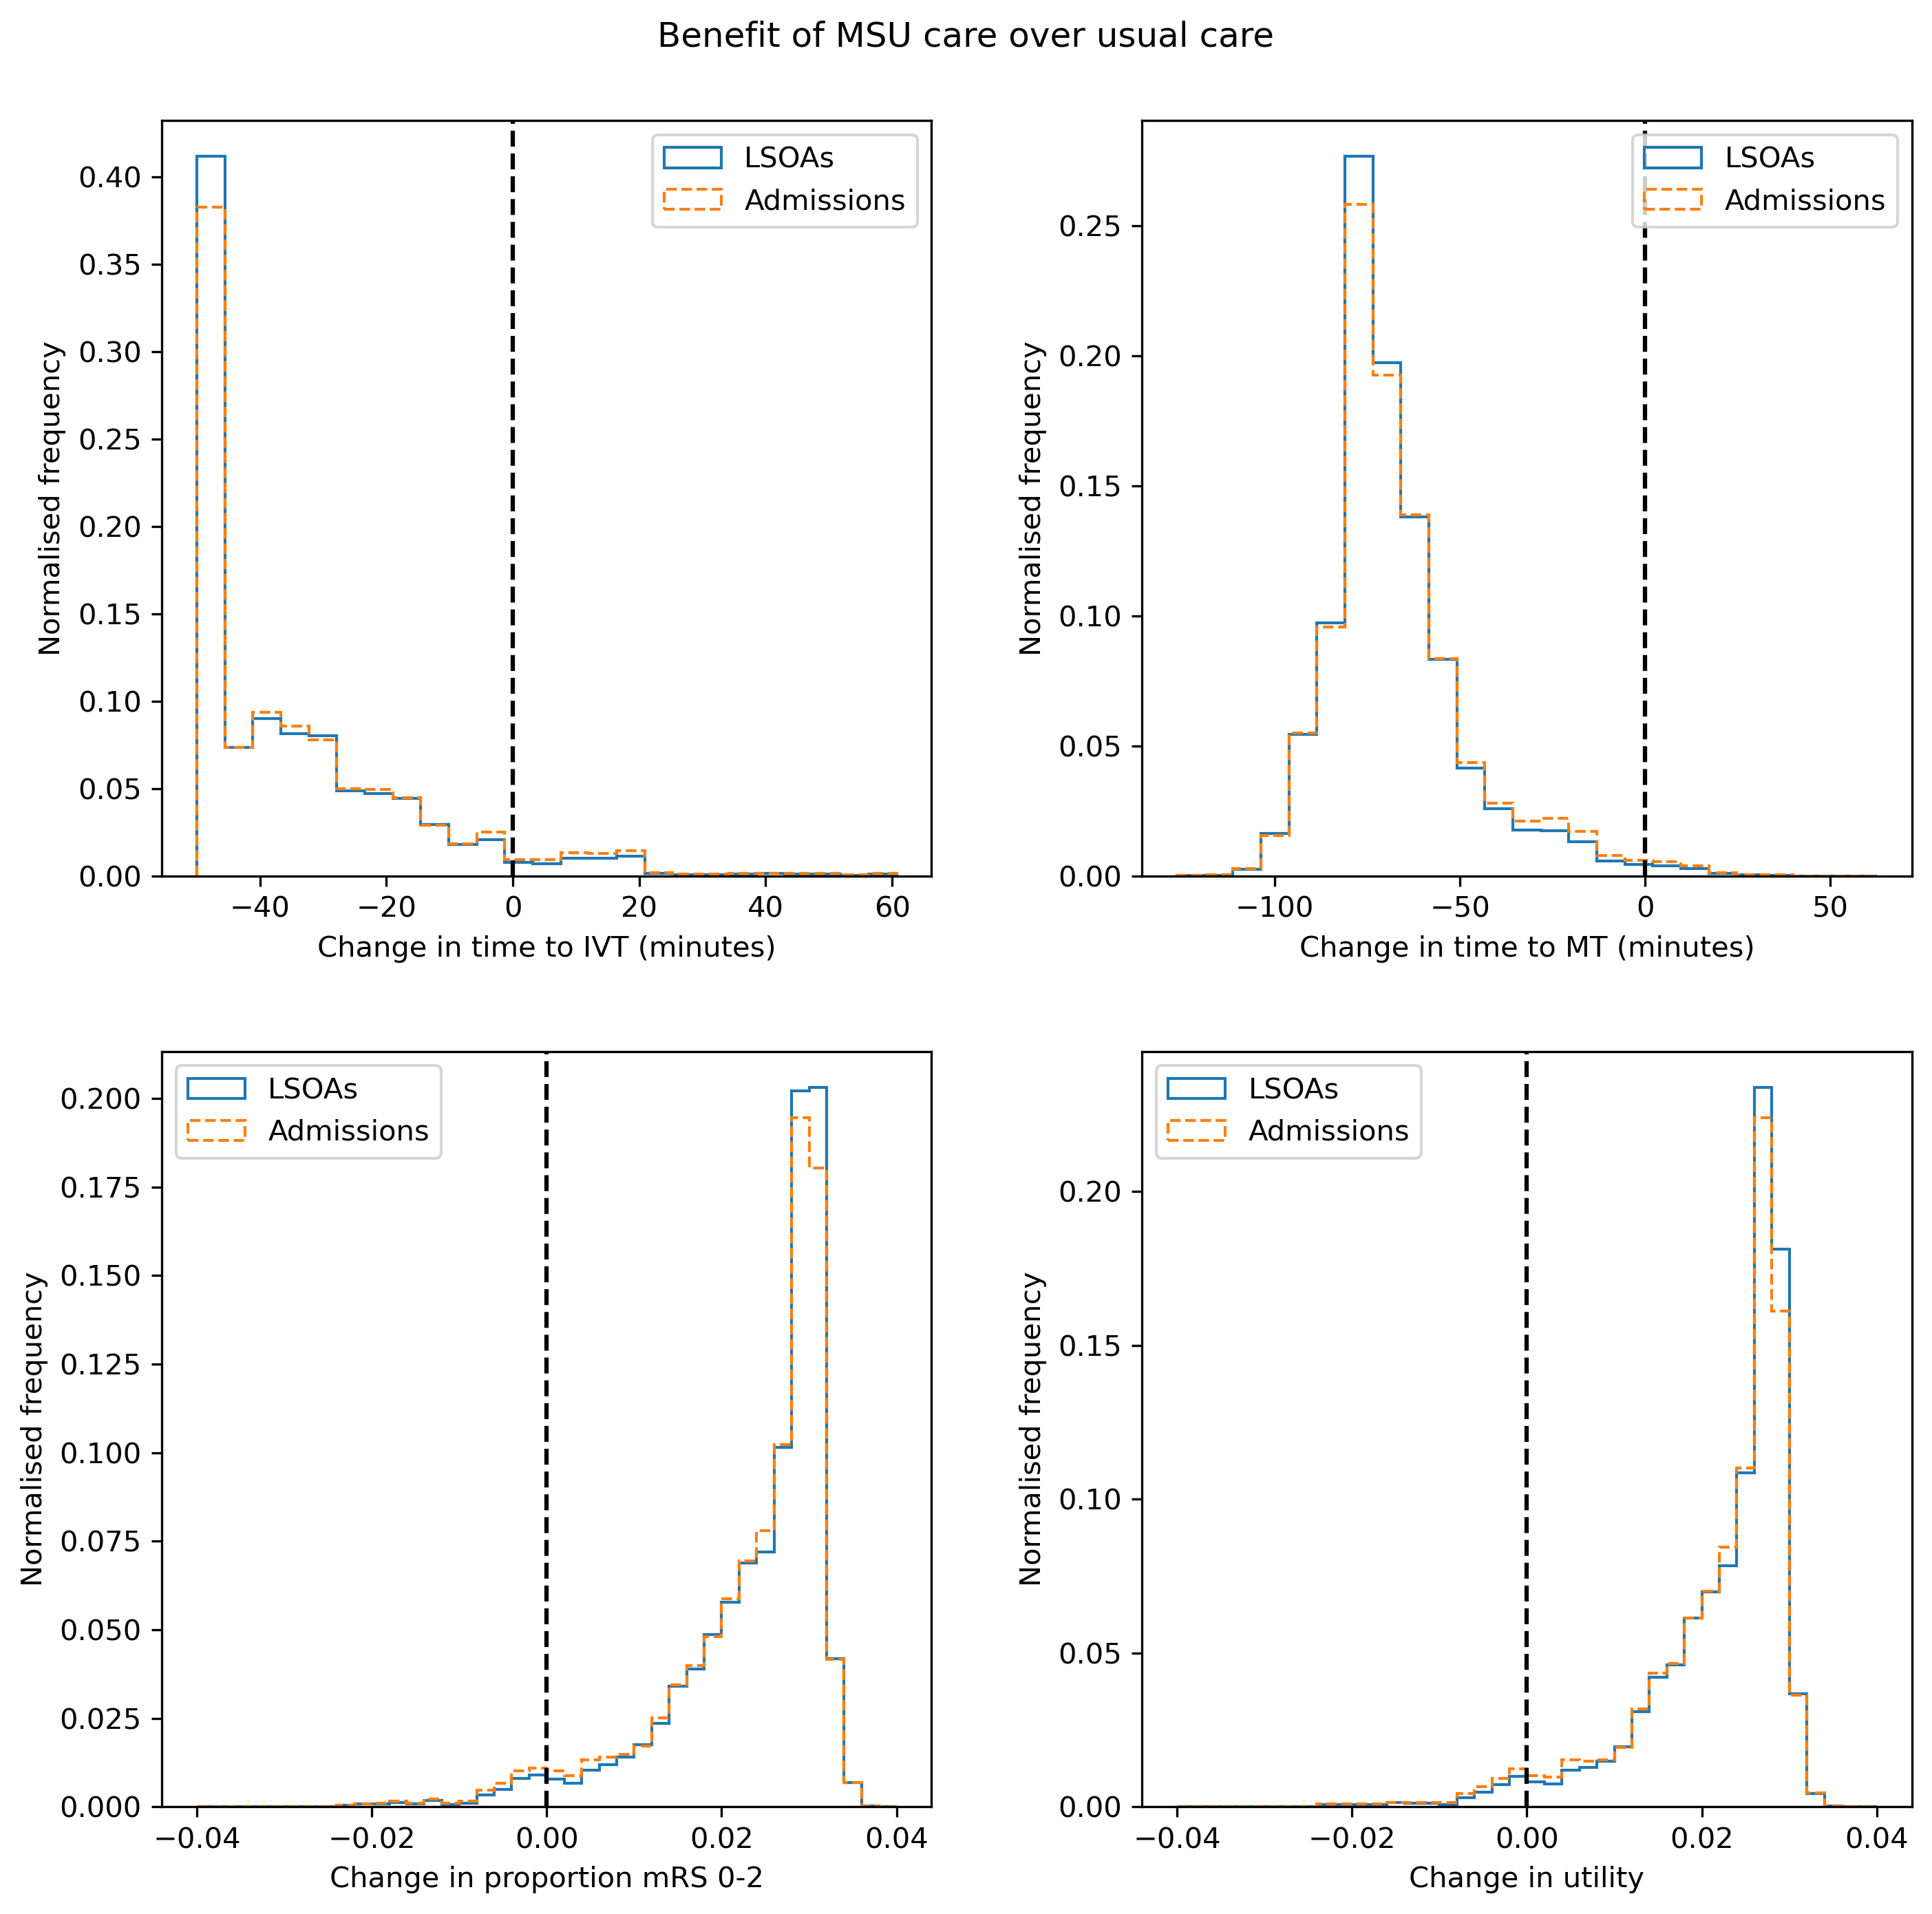
\includegraphics[width=0.75\linewidth]{images/histograms.png}
    \caption{Distribution of benefit of MSU care over usual care across LSOAs (assuming 70\% nLVO, 30\% LVO in the treated population, with LVO receiving IVT/MT in combination). Benefit is described either as even across LSOAs (solid line), or weighted by admissions by LSOA (dotted line). Histograms show change in time to IVT (top left), time to MT (top right), proportion mRS 0--2 post stroke (bottom left), or utility (bottom right).}
    \label{fig:msu_histograms}
\end{figure}

\subsection{Varying number of MSU base locations}

A greedy algorithm was used to select MSU base locations in which MSU base locations are sequentially added one at a time, with each new location selected based on the best possible improvement in utility by adding one more unit. The utility gain is calculated for those patients treated by an MSU rather than with usual care. As the number of MSU base locations increased, the benefit of MSU care over usual care increased (figure \ref{fig:greedy}), but with diminishing returns. The advantage of MSU care over usual care improved utility by 0.020, 0.024, 0.027, and 0.29 with 10, 25, 50 and 100 MSU base locations when MSU base locations are chosen from any stroke unit type. There were 3 CSCs in the first 10 selections, and 8 CSCs in the first 20 selections. With MSU base locations at the 23 current CSCs, the net utility benefit over usual care was 0.022. With the same number of MSU base locations being selected from any stroke centre type, the utility benefit can be increased to 0.023.

\begin{figure}[h]
    \centering
    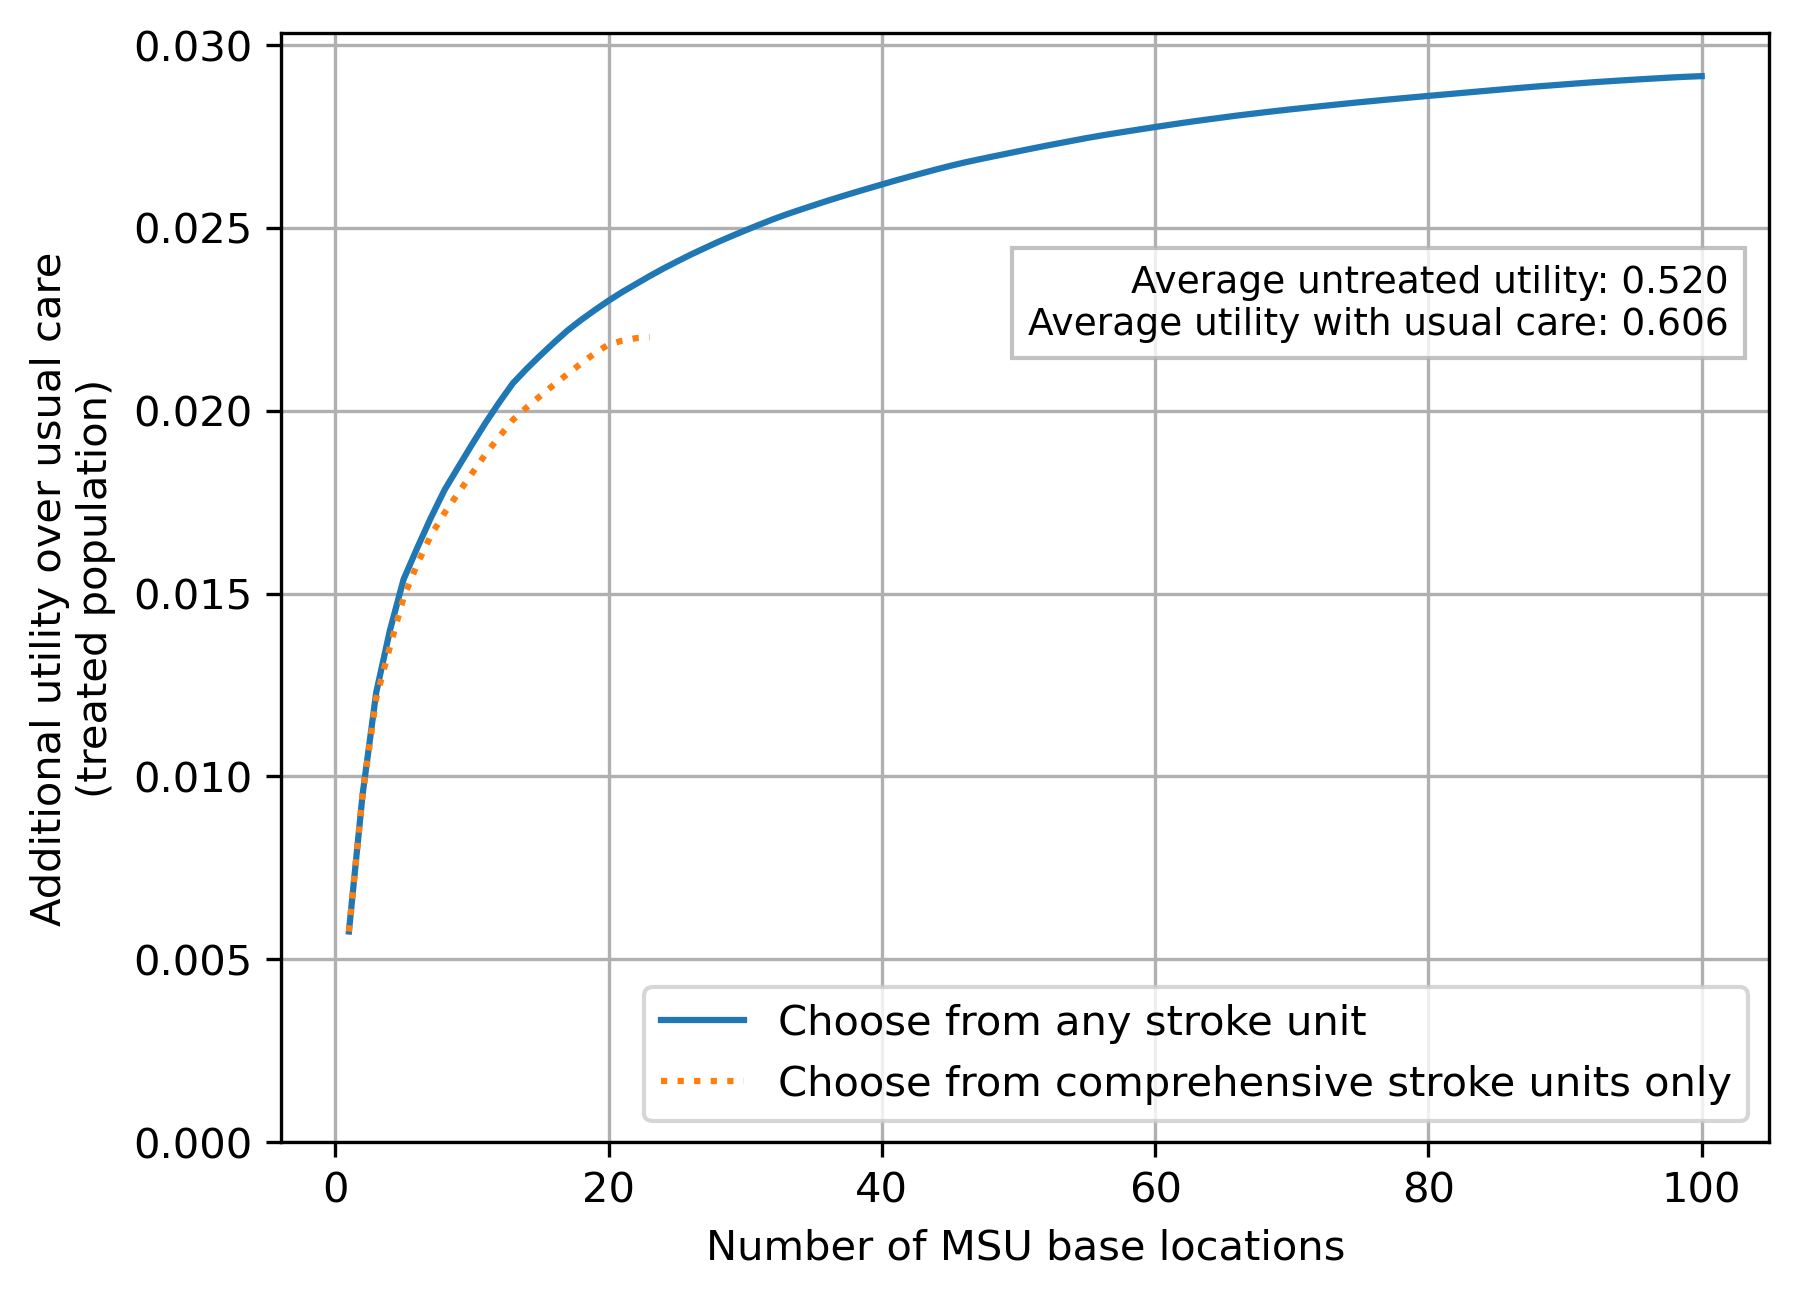
\includegraphics[width=0.5\linewidth]{images/msu_advantages_greedy.png}
    \caption{Increasing number of MSU base locations, with selection by a greedy algorithm based on improvements in utility. The additional utility is for those patients treated by MSU rather than usual care. Units were chosen either from any stroke centre type (solid line) or only from CSCs (dashed line). Utility for the untreated population was 0.520, which was increased to 0.602 with usual care.}
    \label{fig:greedy}
\end{figure}

\subsection{Proportion of patients receiving reperfusion}

In our modelling we have focussed on the benefit for those who receive IVT or MT. Overall, the central probability across realistic scenarios is one extra independent-living outcome for every 50 patients treated. IVT and MT rates vary significantly between countries \cite{kim_global_2024}, but we might take a realistic target of 20\% of patients receiving IVT or MT, in which case there would be one extra independent-living outcome for every 250 confirmed stroke patients (ischaemic and haemorrhagic) where the MSU is dispatched. Not all patients suspected of having stroke at ambulance dispatch will have a confirmed stroke; positive predicted value of suspected stroke at emergency dispatch is about 50\% \cite{kim_global_2024}, in which case there would be one extra independent-living outcome for every 500 of all patients to whom the MSU is dispatched.

%\section{Discussion}

% Key findings

MSUs have been shown to have clear benefit in metropolitan areas \cite{fatima_mobile_2020, chen_systematic_2022}. Our focus has been on predicting the benefit (or disbenefit) of MSUs across a wider geography, where MSUs may have poorer response times, but may still benefit particular patients by faster direct access to a MT-capable centre. To understand these complex geographic effects we have chosen to use modelling, based on predicting outcomes depending on times to both IVT and MT. The modelling of clinical effect was performed by synthesising known relationships between treatment times and outcomes for IVT and MT, while also extending the predictions to the expected mix of patients in real-world settings. By predicting the full range of mRS scores we can also estimate utility scores with different treatment options.

In this first study to model implementation of MSUs across a whole health system, overall we found a relatively marginal predicted benefit from the widespread adoption of MSUs across the whole of England (58 million population). Using plausible process timings we found the magnitude of benefit was likely to be an increase of 0.015 to 0.030 in health utility or 0.015-0.030 in the proportion of independent patients at 6 months. The benefit to patients with nLVO was around 0.015 in the two measures. The benefit to patients with LVO was larger (around 0.035 in the two measures), with the majority of this benefit coming from the direct conveyance of patients with LVO to a MT-capable centre, avoiding the need for inter-hospital transfers and their associated delays, though it is possible that those delays may be reduced by optimisation of other aspects of the current pathway. The benefit from earlier IVT is similar to that modelled by Holodinsky et al. \cite{holodinsky_jessalyn_k_what_2020}. Benefit was larger in the regions within reasonable travel distances of the MSU, which would have similar catchments to those in the clinical trials of MSUs.

We have directly modelled only the ischaemic stroke population treated with IVT or MT. The overall net benefit will be diluted by patients the MSU is dispatched to who are either stroke patients who do not receive or are excluded from IVT or MT (including those with haemorrhage), or who are not confirmed to have had a stroke. In the treated population, across all of England, for every 100 patients suitable for IVT or MT, there will likely be 1-3 more people who can live independently because of earlier treatment. If only about 1 in 5 stroke patients are suitable candidates for IVT or MT, the MSU would need to attend approximately 250 stroke patients for every one extra independent-living outcome. If about half of the patients whom the MSU is dispatched to are actual strokes (the others being stroke mimics), the MSU would need to attend approximately 500 patients for every one extra independent-living outcome. 

We found that the benefit of MSU care over usual care was critically dependent on rapid dispatch of the MSU and relatively rapid IVT ($\leq$30 minutes) on-scene. MSUs are therefore not an alternative to the optimisation of day-to-day operational activities in ambulances or in hospital. Additionally, if current processes are improved the benefit of MSUs will be diminished. For example, ambulance on-scene times have been reported to have a median value of 33 minutes in a UK setting \cite{mcclelland_what_2023}, compared to 15 minutes in a US setting \cite{patel_evaluation_2014}. Therefore, there may be potential to reduce onset-to-treatment times in usual care by at least 15 minutes by optimising usual pre-hospital care.

The benefit of MSU care diminished with distance from the MSU base location, though there was a halo effect for patients with LVO, with patients benefiting from direct transfer to MT-capable centres without excessive MSU arrival times. The diminishing benefit of MSUs is similar to that observed in clinical trials, where in Berlin the advantage of MSU care over usual care, when considering time to treatment, fell with distance from the MSU base location \cite{koch_influence_2016}. MSUs centred in metropolitan areas are therefore not a solution to significantly improving stroke outcomes in more remote locations. However if MSUs were based in remote locations there would be a challenge of long MSU travel times if the MSU is to maximise the number of patients seen each day. Additionally, MSUs will only partially solve the challenge of timely access to MT from remote areas. Maximising the net benefit of MSUs may therefore be at the cost of worsening equity of access to emergency stroke reperfusion therapies, as when MSUs are placed in metropolitan areas they improve access to care for those that already have the best access. Therefore care providers should also consider combining MSUs with other approaches which could reduce inequity such as CSC configurations and selection of patients for direct admission during standard ambulance assessment. 

We modelled net delays in MT of 15-90 minutes added to the inter-hospital travel time. In a study of a stroke registry Froehler \textit{et al.} found that, on average, MT was delayed by 75 minutes plus travel time \cite{ froehler_interhospital_2017}. Our exploration of possible delay times is biased more towards these processes improving as MT becomes more established, but in some particular instances transfer-related delays may be longer, which would improve the benefit of using MSU for patients that are suitable candidates for MT.

As the benefit of CSCs varies with patient location, a possible strategy of deployment of MSUs is to deploy them selectively for areas of maximum benefit, rather than planning to cover all of England.

We have compared MSU care to usual care, which will involve inter-hospital transfer for those patients first attending an IVT-only centre. We saw that a significant part of the benefit from MSU care for patients with LVO came from avoiding such transfers, with the patient being taken directly to a MT-capable centre. Such benefit may be achieved in other ways, such as use of clinical symptom scoring for pre-hospital section of patients likely to benefit from MT, or by achieving large reductions in door-in-door-out times at PSCs \cite{perez_de_la_ossa_effect_2022}.

We have modelled MSUs being based at stroke centres. We compared basing MSUs at just CSCs (offering both IVT and MT) or at any type of stroke centre. The difference between these two approaches was marginal - likely because CSCs tend to be sited within large dense population centres, which gives them rapid access to large numbers of people. It is possible to site MSUs in other locations, such as ambulance stations, though most benefit will accrue from locating them in or near population centres, which is where stroke centres generally exist. As the number of MSU base locations is increased, the possible benefit increases, but with diminishing returns. 

A possible difference between our model and real-world use of MSUs is that we assume a similar propensity for clinicians to give IVT and MT between both MSU care and usual care for patients within the time window for treatment. This assumption allows us to isolate geographic effects. However, we know different stroke clinicians and teams vary in their propensity to use IVT \cite{de_brun_factors_2018, pearn_what_2023}, and there are other organisational barriers to use of IVT \cite{meurer_provider_2011}. It is likely that MSUs will be staffed by clinicians more confident in using IVT, and organisational barriers to IVT delivery may be overcome, and so IVT use may increase not from the altered times to IVT, but by the patient being seen by clinicians more confident in using IVT and in a setting that has eliminated organisational barriers to IVT. This could partly explain why Chen et al. \cite{chen_systematic_2022} found such a significant increase (34\%) in IVT use in MSU trials; it seems unlikely that this degree of change could come just from the modest speed improvements offered by MSU. Another possible reason for higher IVT use in MSUs is that IVT may be ruled out where there are improving stroke symptoms \cite{balucani_mild_2011}, and this probably be less likely to be detected with rapid MSU-based assessment and treatment.

We present results for patients seen by the MSU compared with usual care. A challenge will be identification of the correct patients to dispatch the MSU. In a 2024 review of Emergency Medical Services dispatcher recognition of stroke \cite{wenstrup_emergency_2024}, Wenstrup \textit{et al}. found sensitivity varied from 17.9\% to 83.0\%. Sensitivity median and interquartile range was 56\% (48\%-63\%). Positive predictive value (PPV) was reported in 12 papers and ranged from 24.0\% to 87.7\% with a median and interquartile range of 46\% (42\%-50\%). Typically, therefore, half of stroke patients not identified as such at ambulance dispatch, and only half of suspected stroke patients at dispatch are later confirmed to have a stroke. In one study it was found sensitivity for identifying stroke could be improved, but at the cost of PPV; in a study on the effect of training call handlers \cite{watkins_training_2013}, on 464 patients, sensitivity improved from 63\% to 80\%, but PPV fell from 60.5\% to 39.0\%. Such uncertainty in the sensitivity and PPV of identification of stroke patients makes it difficult to predict how many stroke patients will be seen by MSUs, as that number is limited by both sensitivity of dispatch (where stroke patients are missed) but also by PPV which consumes MSU capacity, risking the MSU not being available as it attends a large number of non-stroke patients. In addition to concerns around identifying patients for MSU dispatch, other implementation concerns have been raised in a qualitative study of clinician views of MSUs \cite{moseley_practitioner_2024}. This includes concerns over how they would be staffed, where they would be based, and whether they will increase or reduce equity of access to emergency stroke care.

Our study adds to the evidence base on how MSUs may affect times to MT, especially when used more widely than areas close to CSCs. When the catchment area of MSUs extends out beyond the usual catchment area of CSCs, the MSU captures patients who would otherwise go to a local IVT-only stroke centre and require onward transfer for MT - effectively functioning as an ambulance redirection intervention. MSUs therefore have potential to improve outcomes for those patients. This effect will be dependent on the MSU using CT-A to identify LVO patients and having reliable image interpretation immediately available. While CT-A has not been routinely used in all MSU models of care, it is increasingly being adopted to improve LVO diagnosis and also to improve MT workflows at the receiving hospital \cite{czap_mobile_2020}. CT-A is likely to be anessential component of MSUs to maximise benefit to patients. 

Estimates of the proportion of stroke patients who have LVO vary. A review by Rennert \textit{et al.} identified estimates of 24\% to 46\% \cite{rennert_epidemiology_2019}. We have used an estimate of 30\% to reflect the likely mix in the reperfusion treated population, but we have separated out benefit for nLVO and LVO so that our results may be interprted for other mixes.

\subsection{Study limitations}

Two key limitations have been discussed: Firstly, we isolated the geographic effects of MSUs and do not model how having an expert specialist team in a well-equipped MSU may increase IVT use simply by being more experienced, and so more confident, in use of IVT. Secondly, due to large uncertainties around sensitivity and PPV of identification of stroke patients for MSU dispatch, we limit our study to modelling of outcomes of those who are seen by the MSU. Real-world benefit will be diluted by stroke patients being missed, or by MSU capacity not being available when required, especially if capacity is constrained by low PPV of suspected stroke at dispatch. Similarly, for the same reason, we do not model how MSUs may affect emergency stroke admission numbers at hospitals (e.g. by changing effective catchment areas). It is possible that widespread use of MSUs could compromise the ability of some smaller hospitals to still provide IVT themselves due to loss of clinicians or experience. We also do not model other potential benefits of MSUs. For example, in haemorrhagic stroke there is potential to start reducing blood pressure sooner where that would benefit patients \cite{li_intensive_2024}. In non-stroke patients it is possible that improved diagnosis by the MSU could help identify the best destination for that patient sooner, or may give more confidence in leaving the patient at home, saving healthcare resources.

We have not modelled selection of late-presenting patients, or patients with unknown stroke onset time. These patients may be selected for IVT or MT based on advanced imaging. These patients would not be expected to follow the decline in effectiveness of IVT or MT described in analysis of how time-to-treatment affects outcomes \cite{emberson_effect_2014, fransen_time_2016}. Further clinical trial data is needed to model how MSUs are likely to affect treatment of late-presenting patients or patients with unknown stroke onset time.

We have modelled MSUs compared with normal care. Alternative proposals for improving pre-hospital stroke care have also been suggested, that we have not sought to model here. For example, alternative approaches to ambulance redirection are available through use of clinical scale assessment triage \cite{dekker_prehospital_2025}, telemedicine \cite{sarpourian_application_2023}, or near patient testing \cite{shaw_rapid_2024}. These alternative methods may offer advantages for patients further away from a MSU base. It is possible, therefore, that the best overall system could be a hybrid of MSU care and alternative methods of care where access to MSU care is likely to be limited.

\section{Conclusions}

Overall we found a relatively small benefit from MSUs across all of England, even with unrestricted MSU capacity. Benefit depends on efficiency of dispatch and treatment, and varies with geography. It is possible that more selective targeting of MSUs could help maximise benefit. A significant part of their potential benefit is derived from avoiding transfers for patients suitable for MT, reducing time to MT significantly. Maximising benefit from MSUs is critically dependent on rapid dispatch and fast on-scene IVT. However, there are other considerations such as resource limitations and implementation challenges, and MSUs should not be seen as an alternative to optimising day-to-day emergency stroke systems.
% References
%\clearpage
%\newpage
%\printbibliography
%\end{refsection}
%\section{Declarations}

\subsection{Ethics approval and consent to participate}

The UK Health Research Authority (HRA) ethics decision tool (\url{https://www.hra-decisiontools.org.uk/}) was used to determine whether ethics approval was required. No ethics/consent was required (as no patients were recruited for this work, and no individual patient data was used).

\subsection{Consent for publication}

Not applicable.

\subsection{Availability of data and materials}

General model code is available at \url{https://github.com/stroke-modelling/muster2}.

Estimated travel times based on patient and hospital locations is available at \url{https://gitlab.com/michaelallen1966/1811_lsoa_to_acute_hospital_travel/}.

Code for estimation of stroke outcome depending on time to IVT or MT is available at \url{https://github.com/samuel-book/stroke_outcome/}, and is available as a Python package at \url{https://pypi.org/project/stroke-outcome/}.

Full results for scenario analysis may be found at \url{https://github.com/stroke-modelling/muster2/tree/main/output}. Full geographic results for mapping mapping may be found at \url{https://github.com/stroke-modelling/muster2/tree/main/map}.

\subsection*{Competing interests}

GF reports receiving consulting fees from AstraZeneca for management of stroke due to intracerebral haemorrhage (payment to his employer), Bayer for lecture on models of NHS industry working, CSL Behring for stroke trial consultancy, and being Chief Executive of Health Innovation Oxford and Thames Valley which has multiple joint working agreements and medical education grants with industry partners that are contracts with Oxford University Hospitals NHS Trust the host organisation for Health Innovation Oxford and Thames Valley.

\subsection{Authors' contributions}

All authors were involved in the design of the models, and in review/editing of the manuscript.

AL, MA, and KP, coded the models. AL and MA were the primary authors of the paper.


\subsection*{Funding}

This work was funded by National Institute for Health and Care Research (NIHR) Health Services and Delivery Research (Reference NIHR153982). MA was additionally funded by the NIHR Applied Research Collaboration South West Peninsula.

The views expressed in this publication are those of the authors and not necessarily those
of the NIHR or the Department of Health and Social Care.

\subsection*{Acknowledgments}

We thank all participants in co-production workshops which helped to inform the modelling described herein.


%\begin{figure}[h]
    \centering
    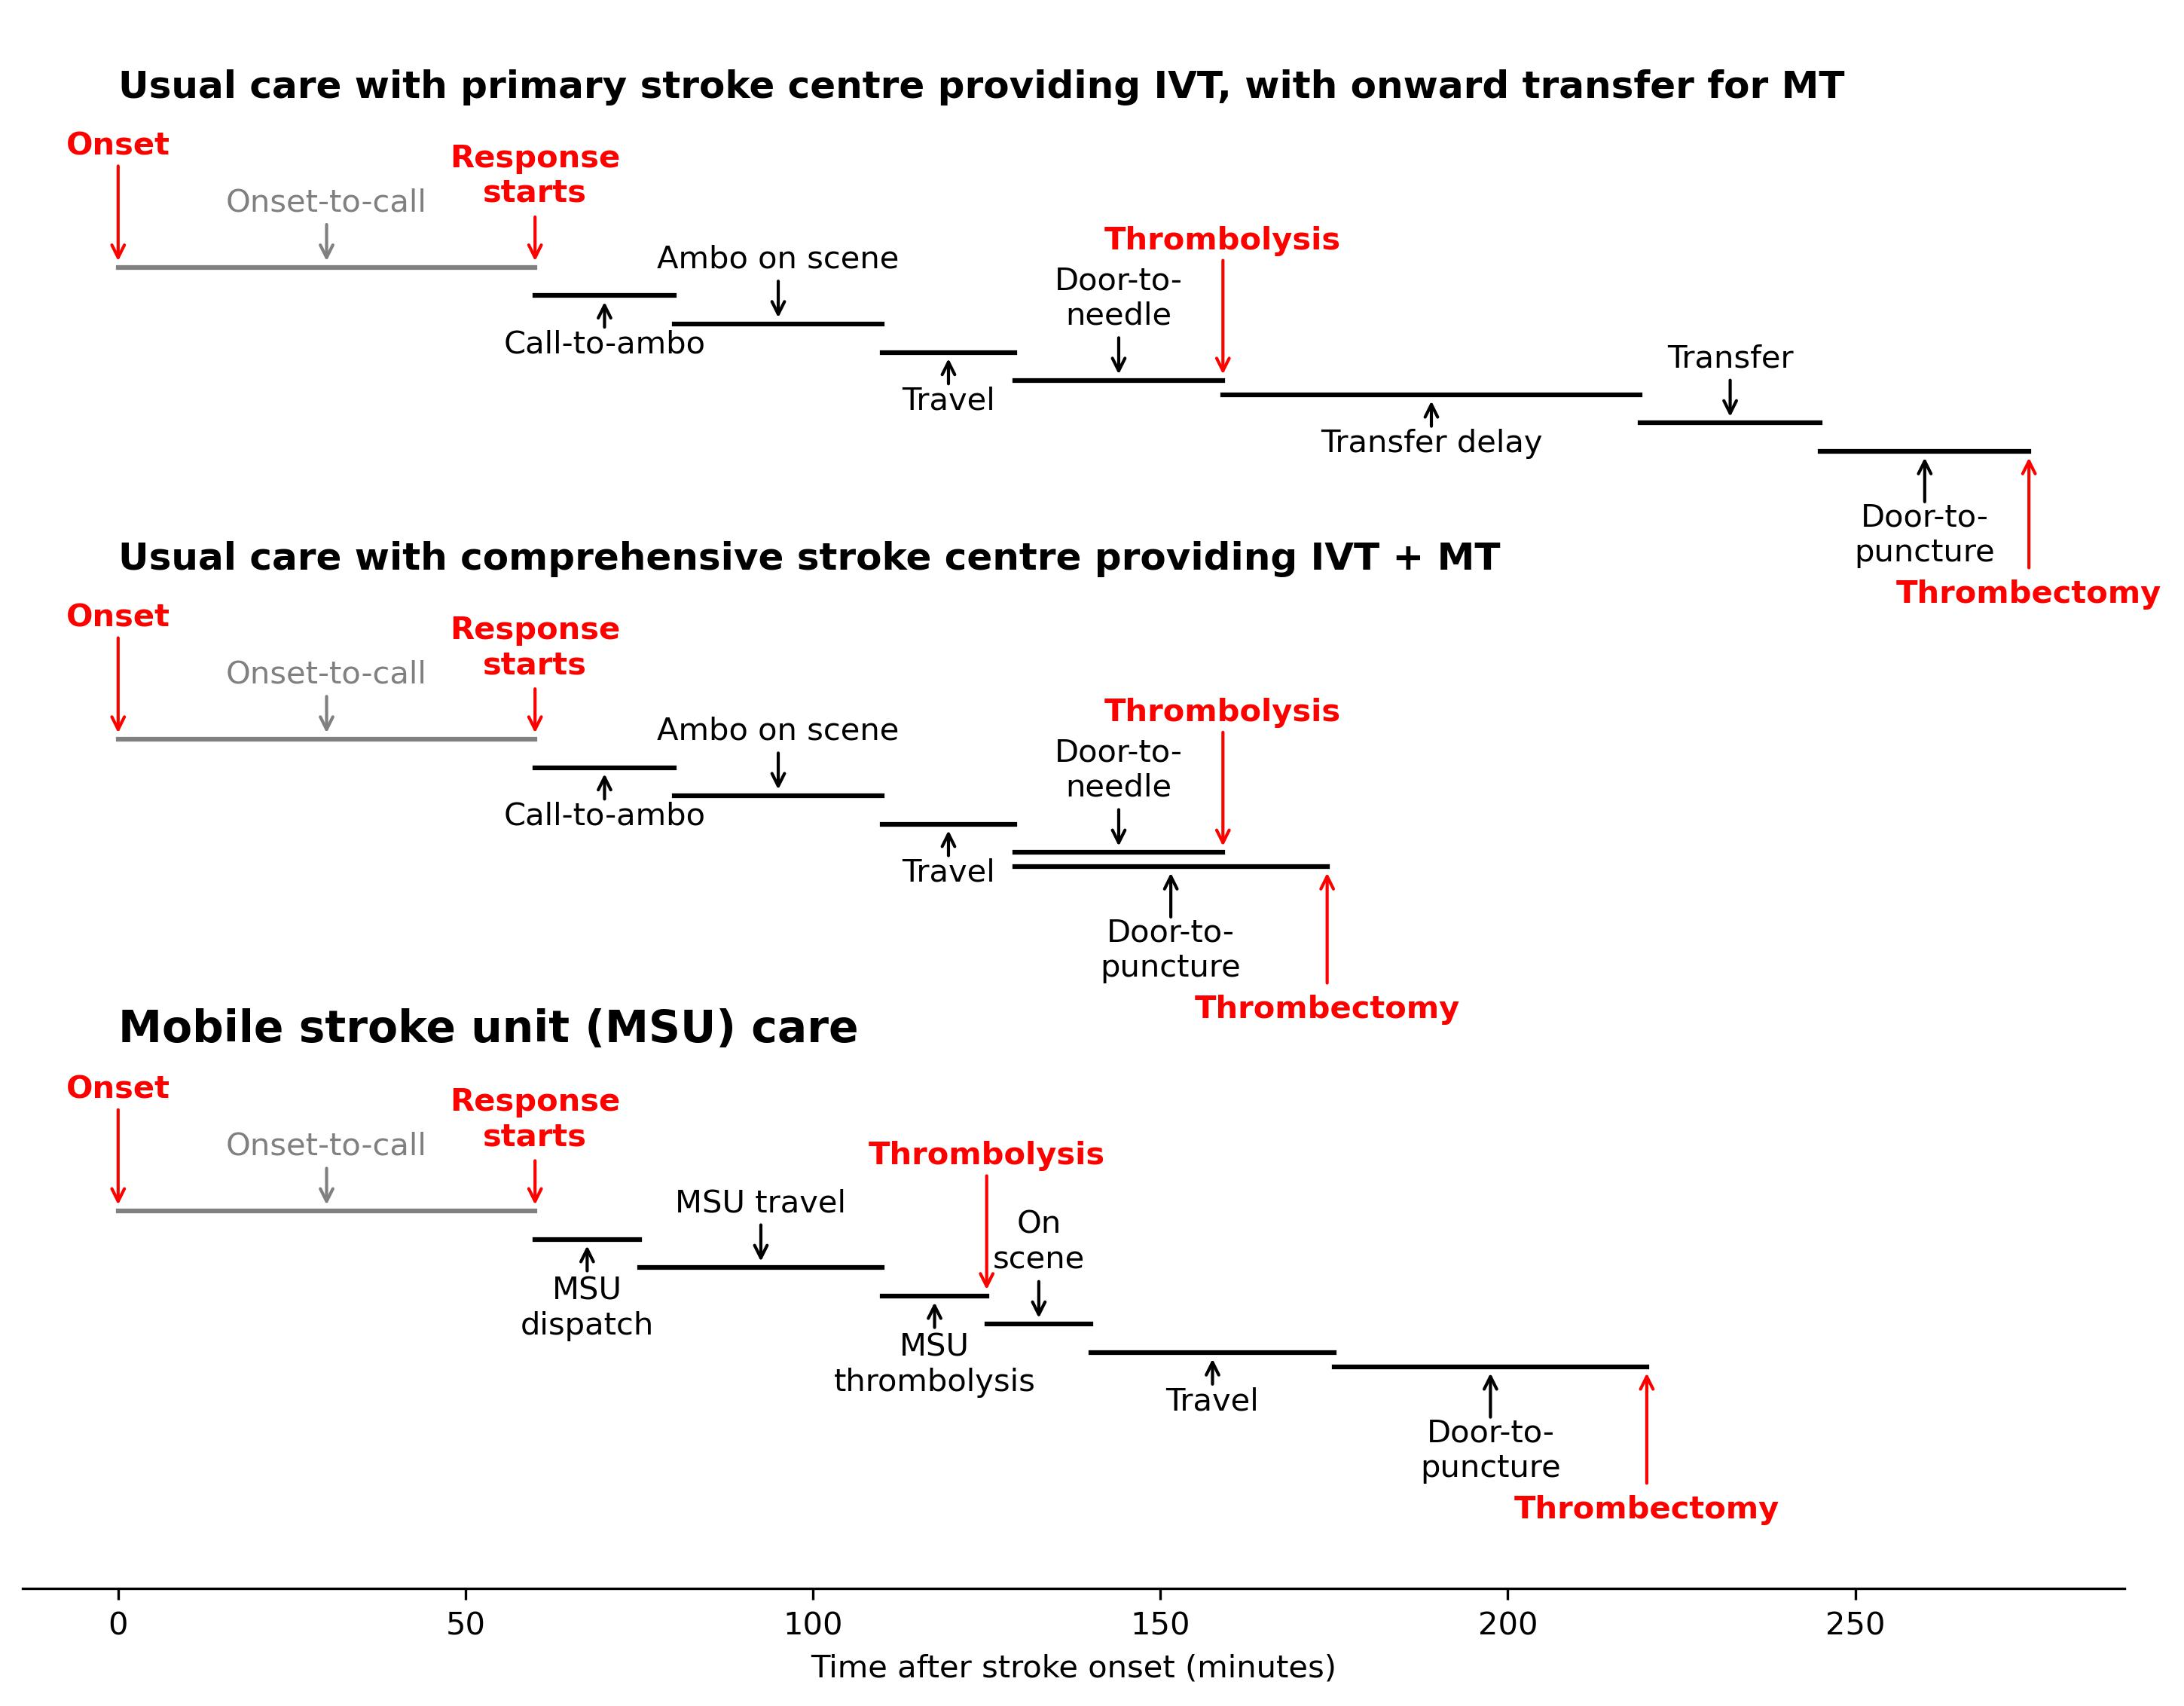
\includegraphics[width=0.85\linewidth]{images/stroke_treatment.jpg}
    \caption{An illustrative timeline showing processes included in the three pathways that are modelled for provision of IVT and MT. Top: Usual care pathway for patients with a PSC closest to their home LSOA, with the PSC providing IVT, followed by the LVO patients having a transfer to the nearest CSC for MT. Middle: Usual care pathway for patients with a CSC closest to their home LSOA, with the CSC providing both IVT and MT. Bottom: MSU care pathway, with IVT provided on-scene by the MSU, followed by the MSU transferring the LVO patients to the nearest CSC for MT. Process times other than travel times are common for all patients (defined by the scenario). Travel times depend on locations of patient and hospitals, with results calculated for all LSOAs in England.}
    \label{fig:process}
\end{figure}

\begin{figure}[h!]
    \centering
    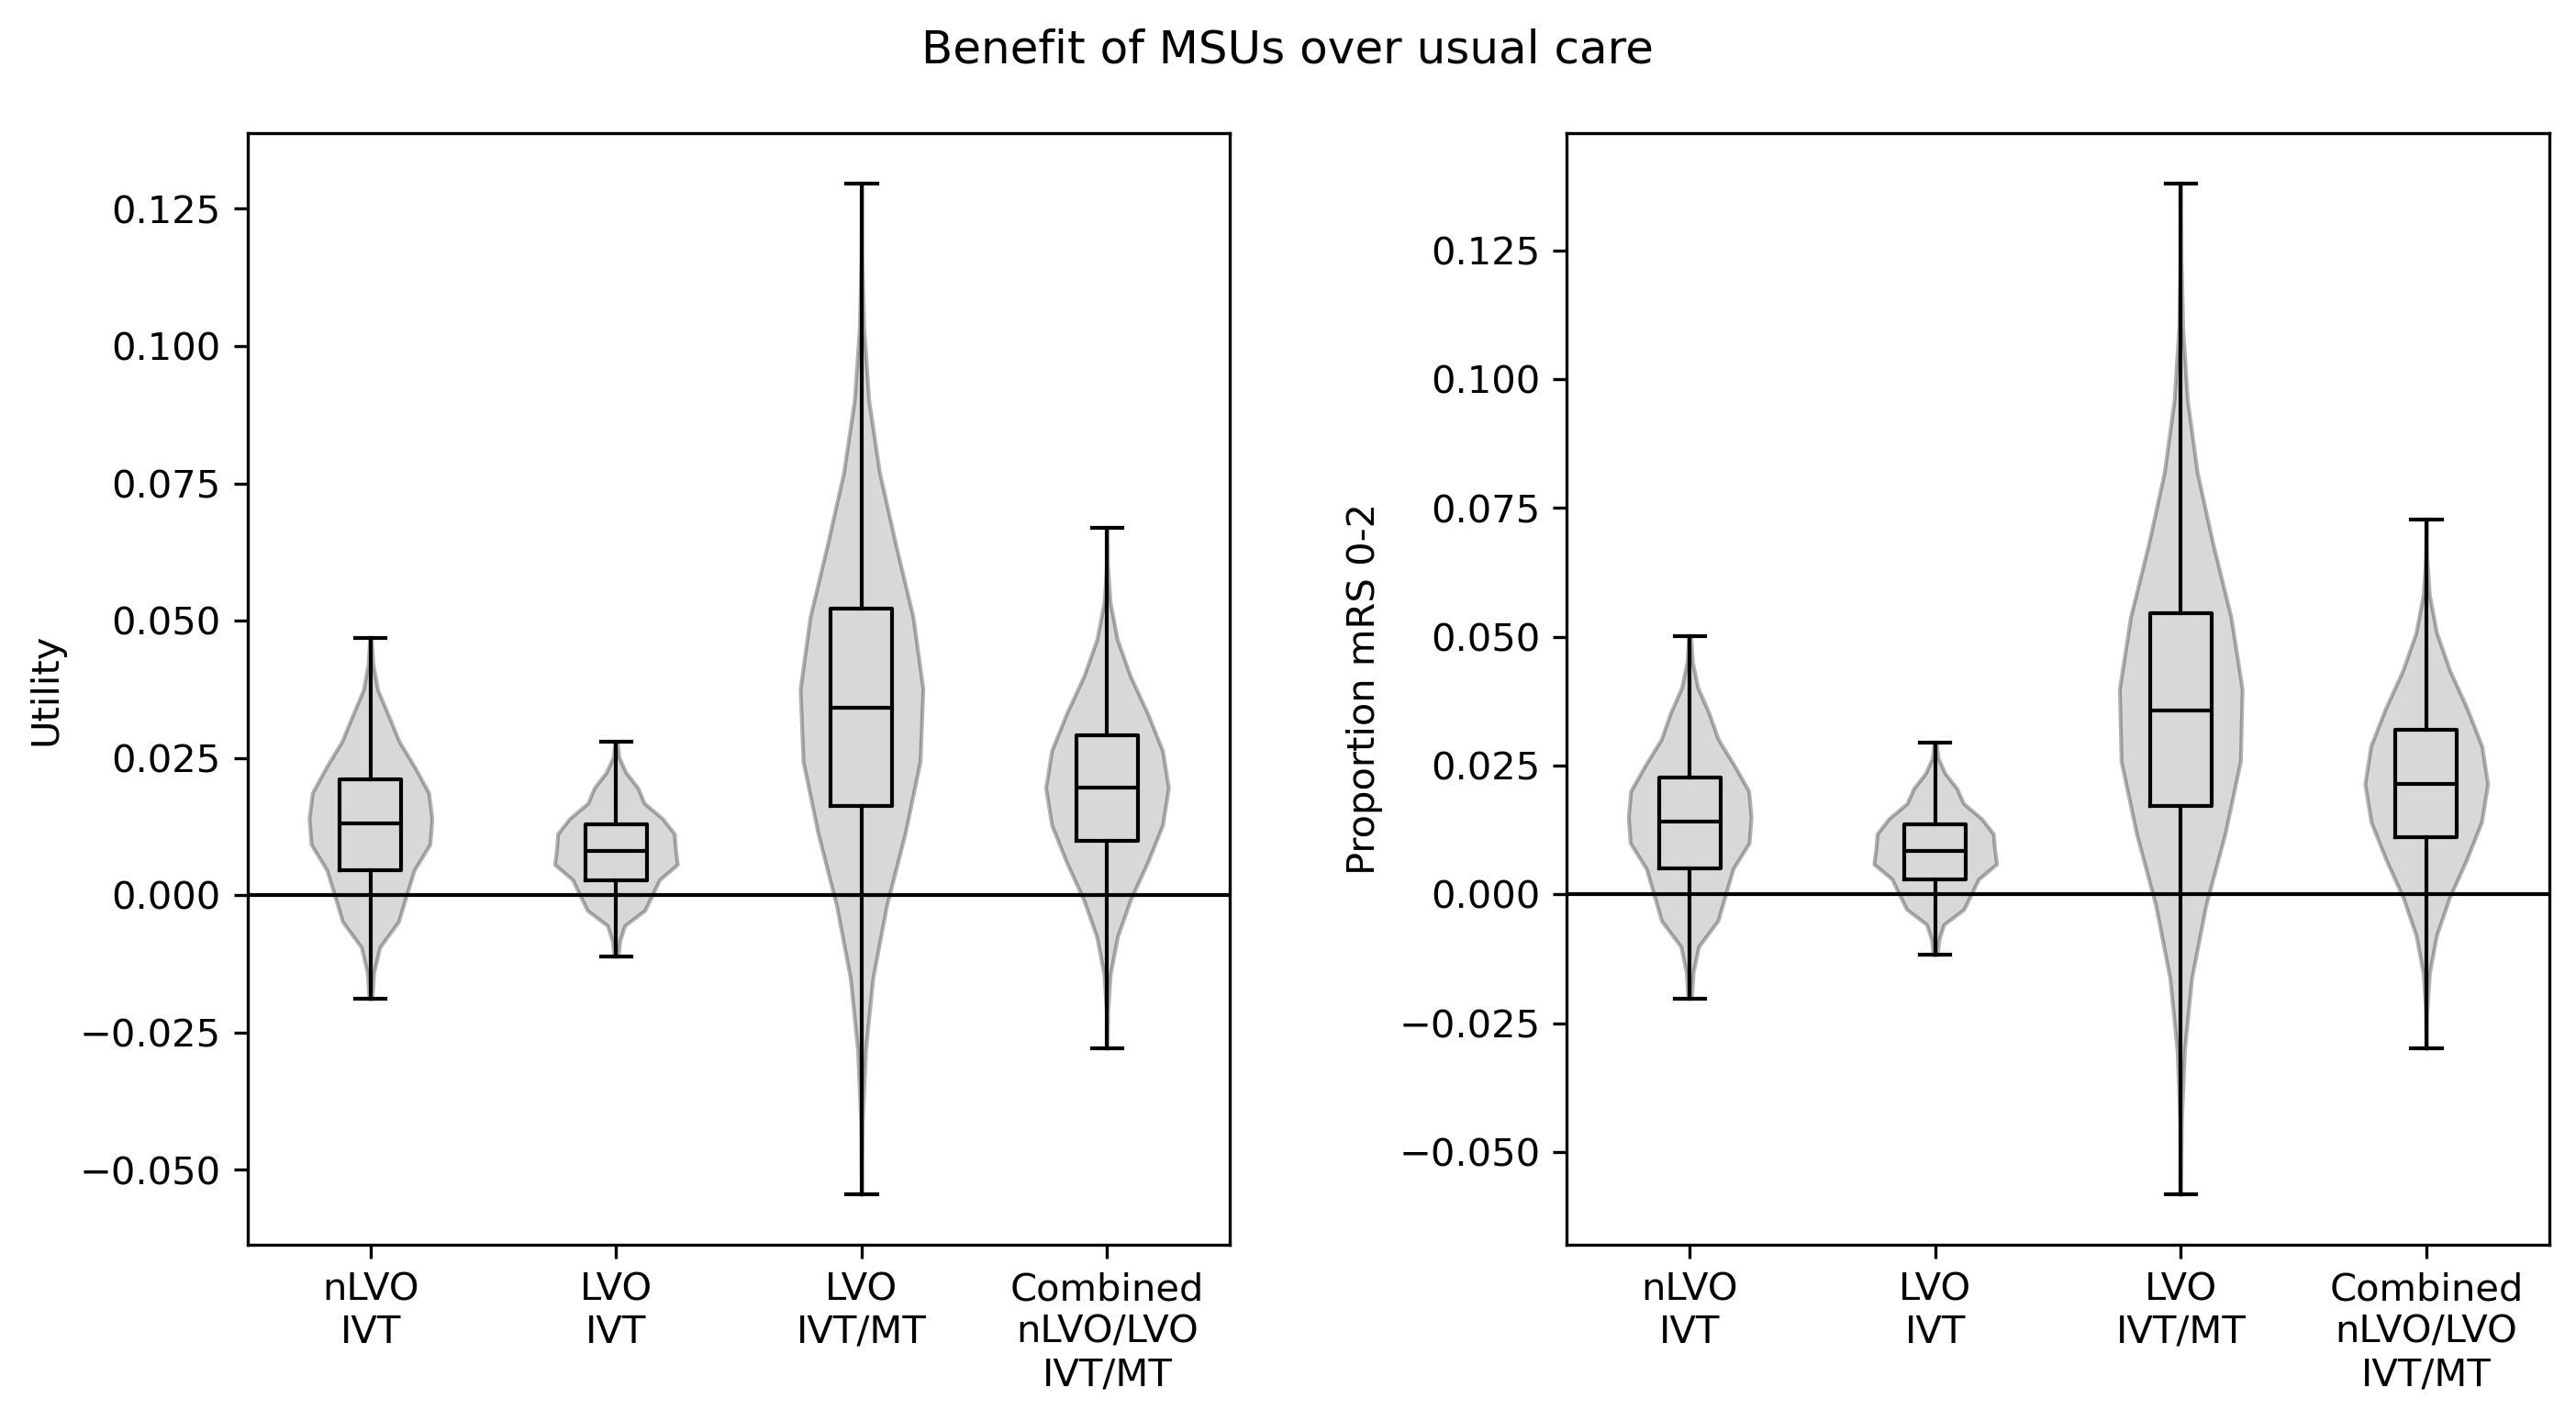
\includegraphics[width=0.75\linewidth]{images/scenario_results_summary.png}
    \caption{Benefit of MSU care over usual care across all scenarios (exploring the effect of changing process durations), in the treated population, measured by utility (left) or the proportion of patients with an outcome of mRS 0-2 (right), separating the changes for patients with nLVO and LVO. Results for LVO patients show the effect of MSU care on the benefit derived from IVT alone, or by IVT/MT in combination. Box plots show range, interquartile range, and median across all scenarios. The combined nLVO/LVO benefit assumed 70\% nLVO and 30\% LVO in the treated population, with LVOs receiving IVT/MT in combination. Overlaid over the box plots are violin plots showing the distribution of results across all scenarios. A positive value indicates MSU care provides an advantage over usual care, and a negative value indicates MSU care is disadvantageous compared with usual care. Results are the average effect across all LSOAs in England.}
    \label{fig:scenarios_overview}
    
\end{figure}
\begin{figure}[h!]
    \centering
    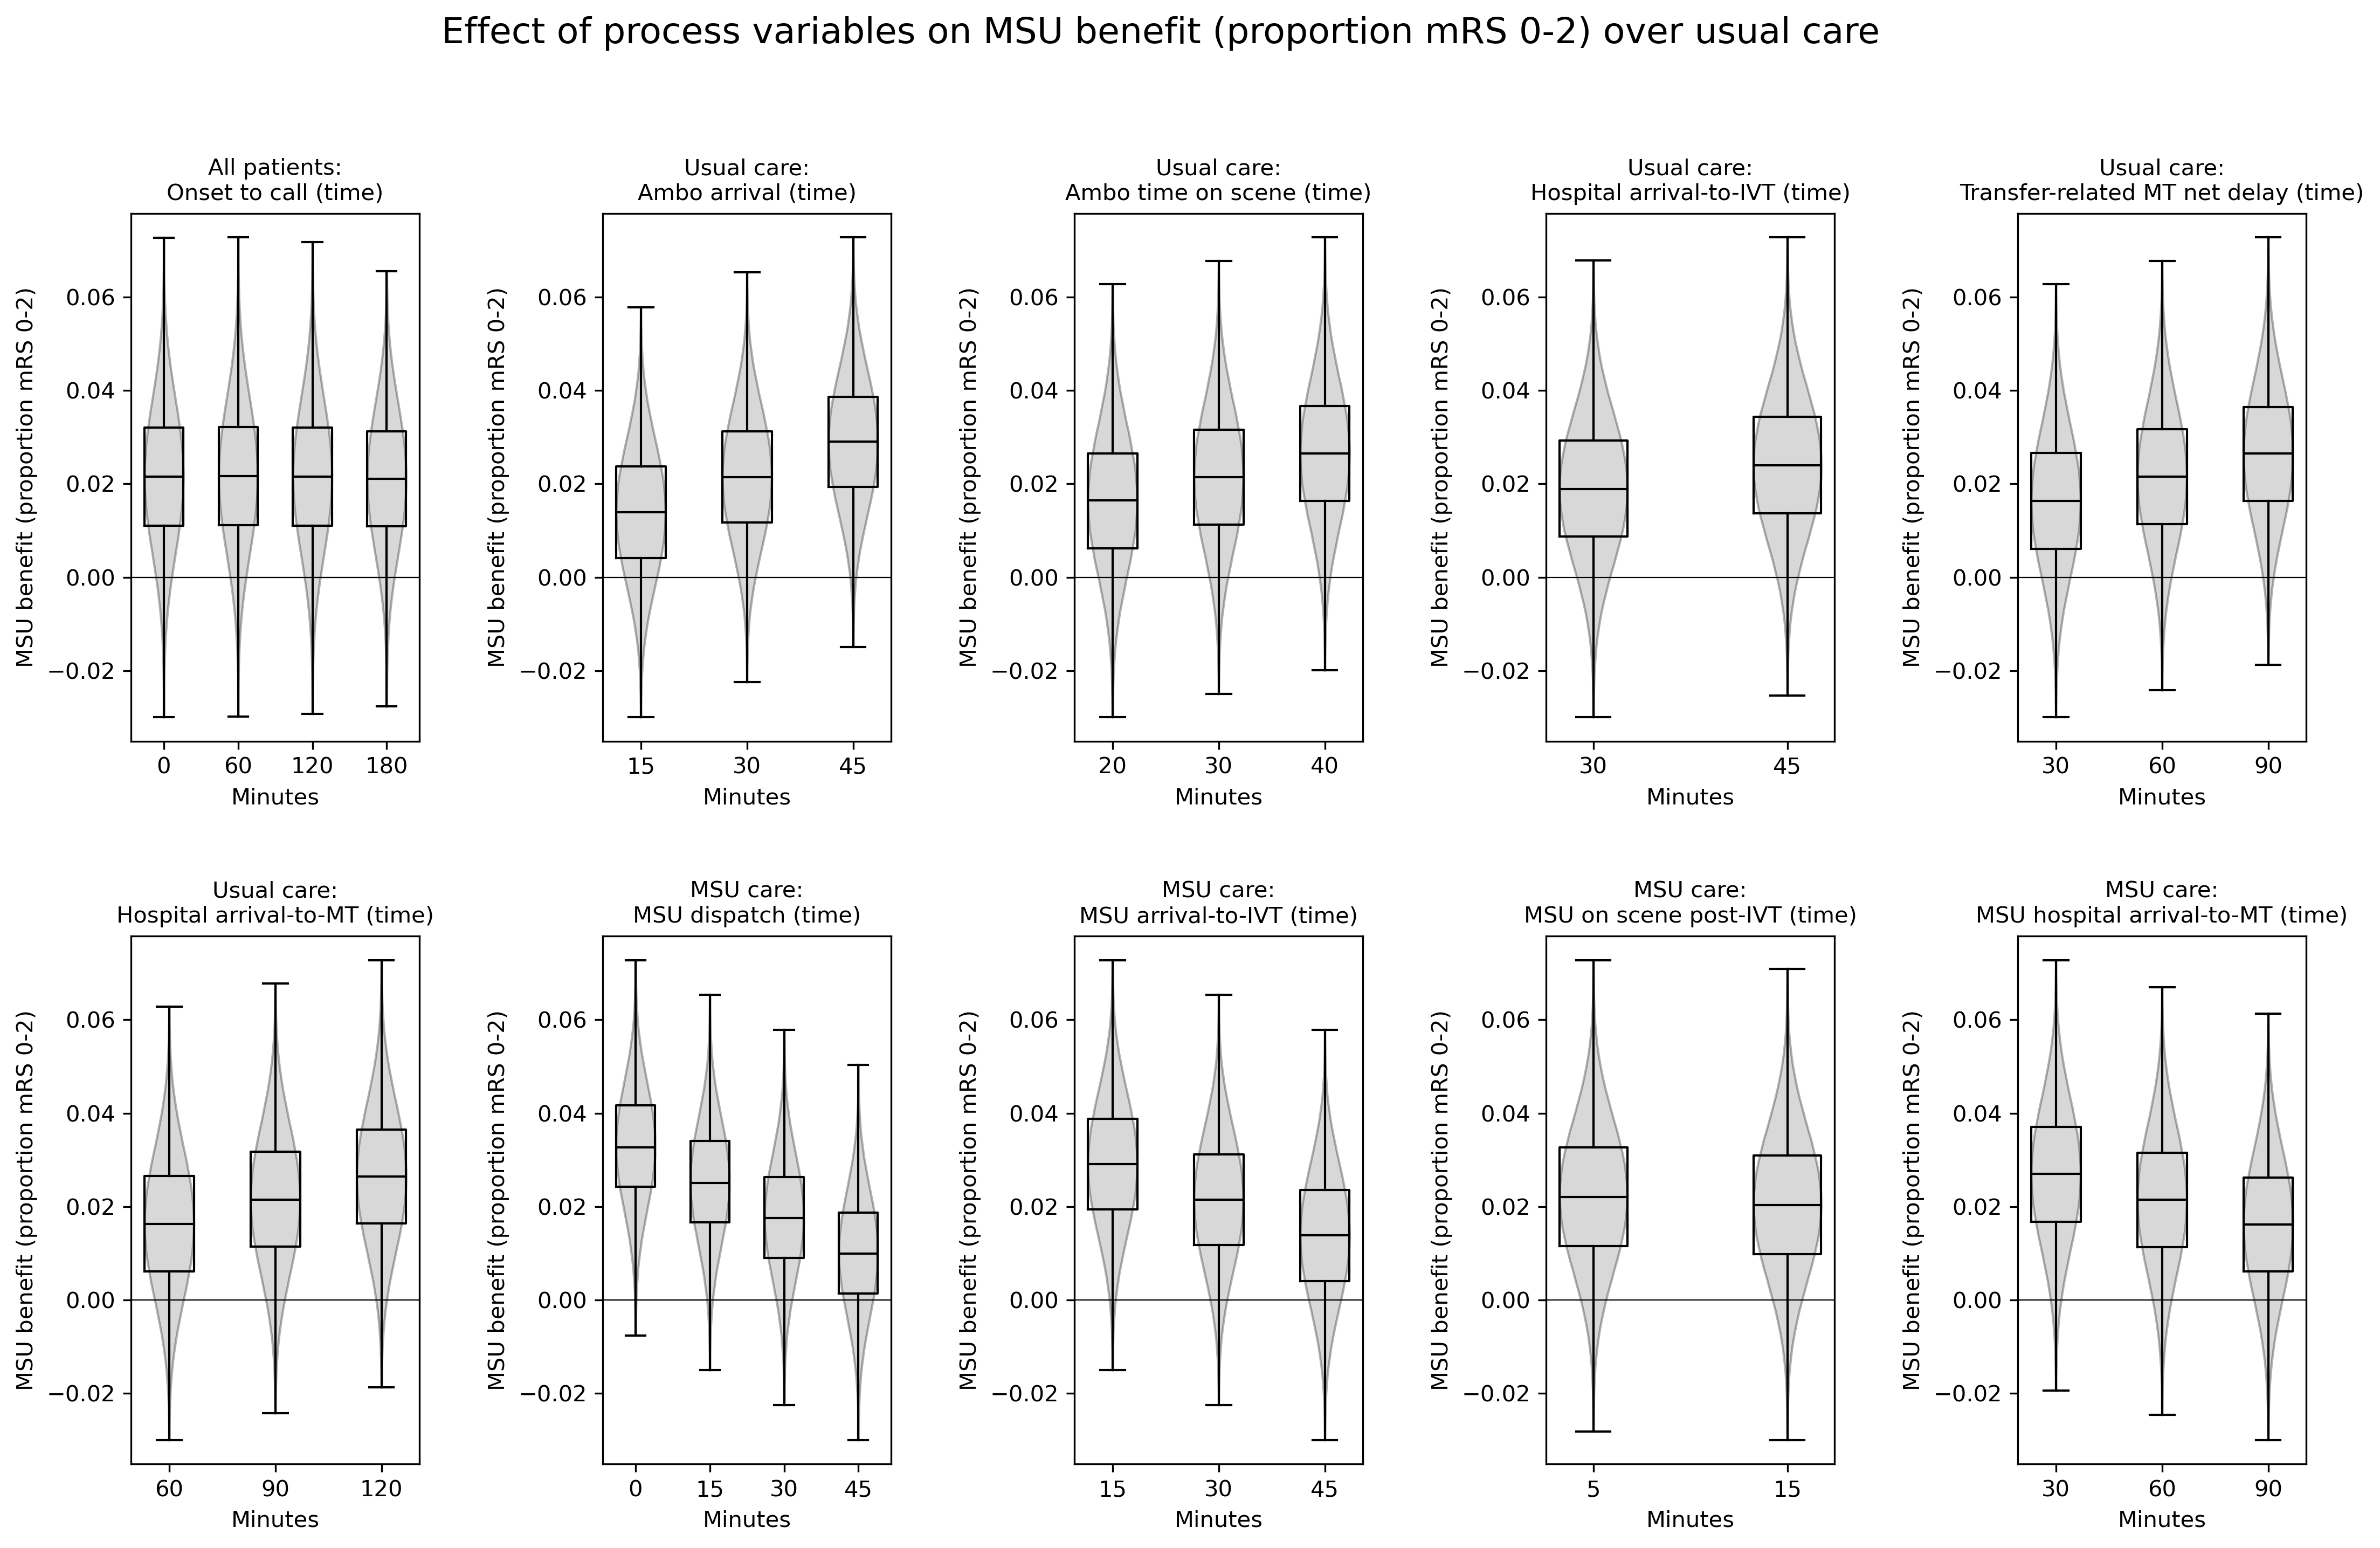
\includegraphics[width=1\linewidth]{images/msu_net_mrs_0-2_benefit.png}
    \caption{The effect of changing modelled process durations on the predicted benefit of MSU care over usual care, in the treated population (comprised of 30\% nLVO and 70\% LVO patients, where nLVO patients receive IVT and LVO patients receive IVT followed by MT), measured by proportion of patients with an outcome of mRS 0-2. For each target parameter, results are averaged across all scenarios with that given parameter value. Box plots show range, interquartile range, and median, across all scenarios. Overlaid over the box plots are violin plots showing the distribution of results across all scenarios. Results are the average effect across all LSOAs in England.}
    \label{fig:scenarios_mrs}
\end{figure}

\begin{figure}[h!]
    \centering
    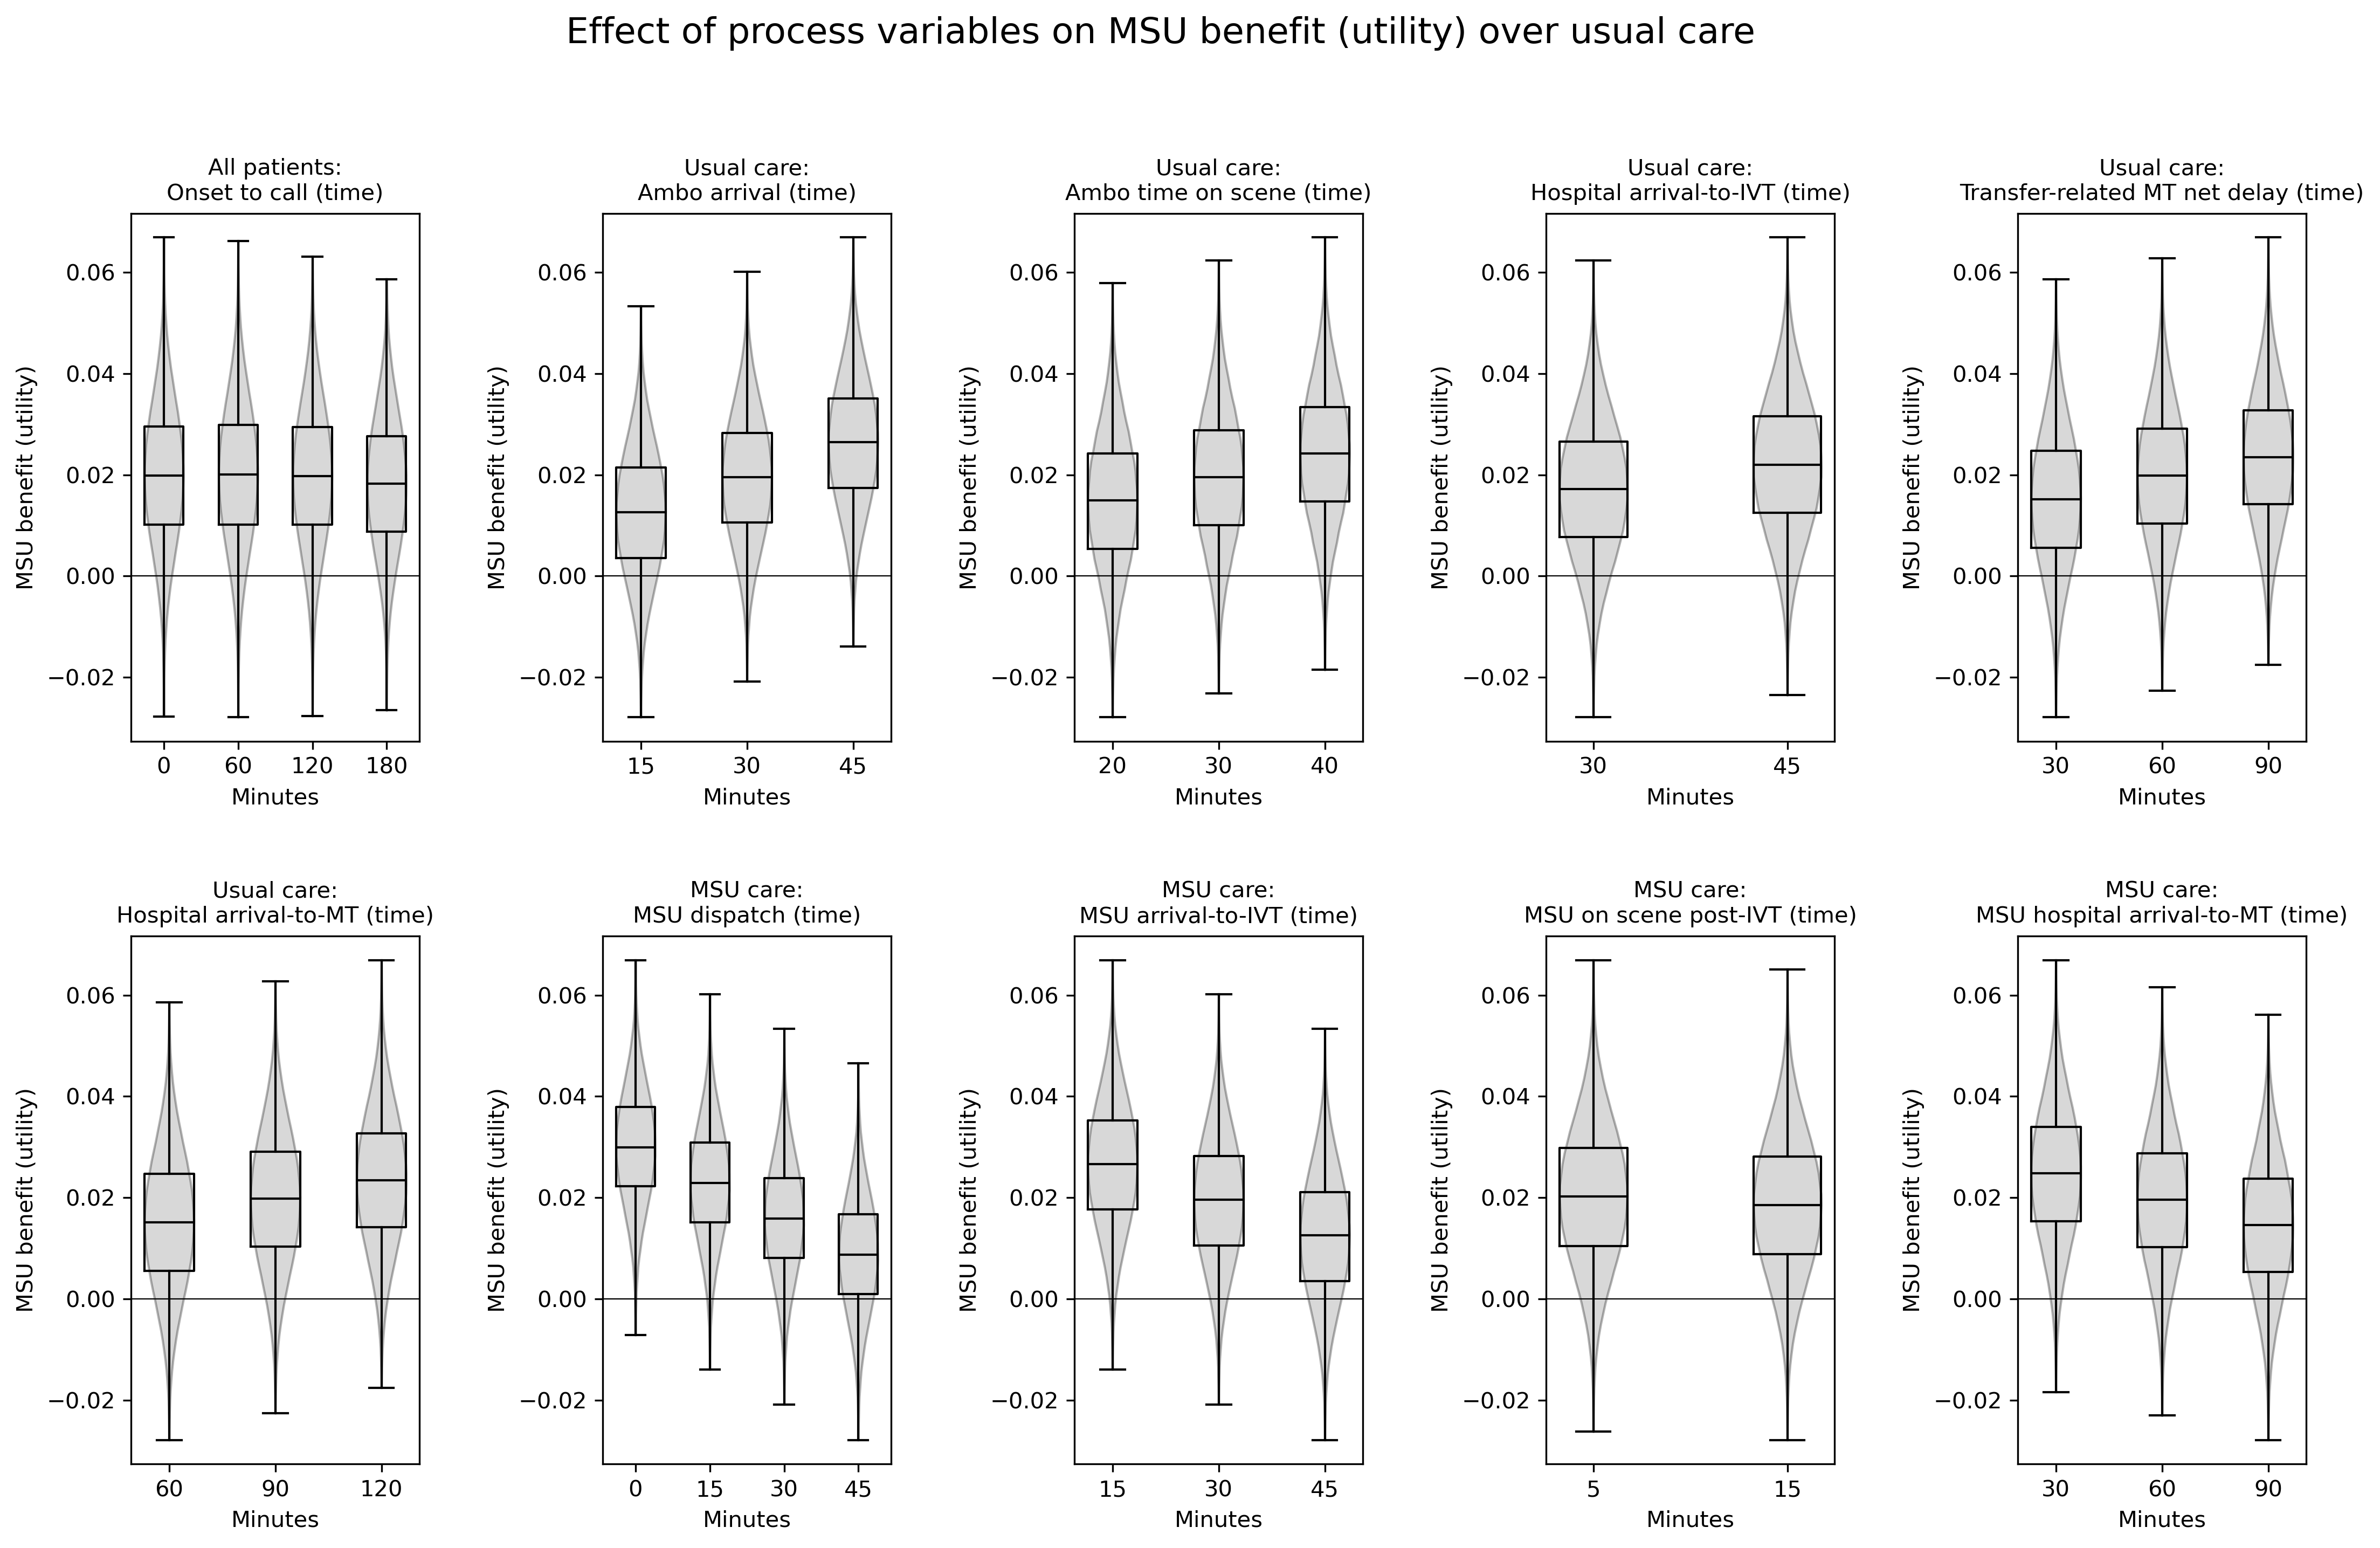
\includegraphics[width=1\linewidth]{images/msu_net_utility_benefit.png}
    \caption{The effect of changing modelled process durations on the predicted benefit of MSU care over usual care, in the treated population (comprised of 30\% nLVO and 70\% LVO patients, where nLVO patients receive IVT and LVO patients receive IVT followed by MT), measured by utility. For each target parameter, results are averaged across all scenarios with that given parameter value. Box plots show range, interquartile range, and median, across all scenarios. Overlaid over the box plots are violin plots showing the distribution of results across all scenarios. Results are the average effect across all LSOAs in England.}
    \label{fig:scenarios_utility}
\end{figure}

\begin{figure}[h!]
    \centering
    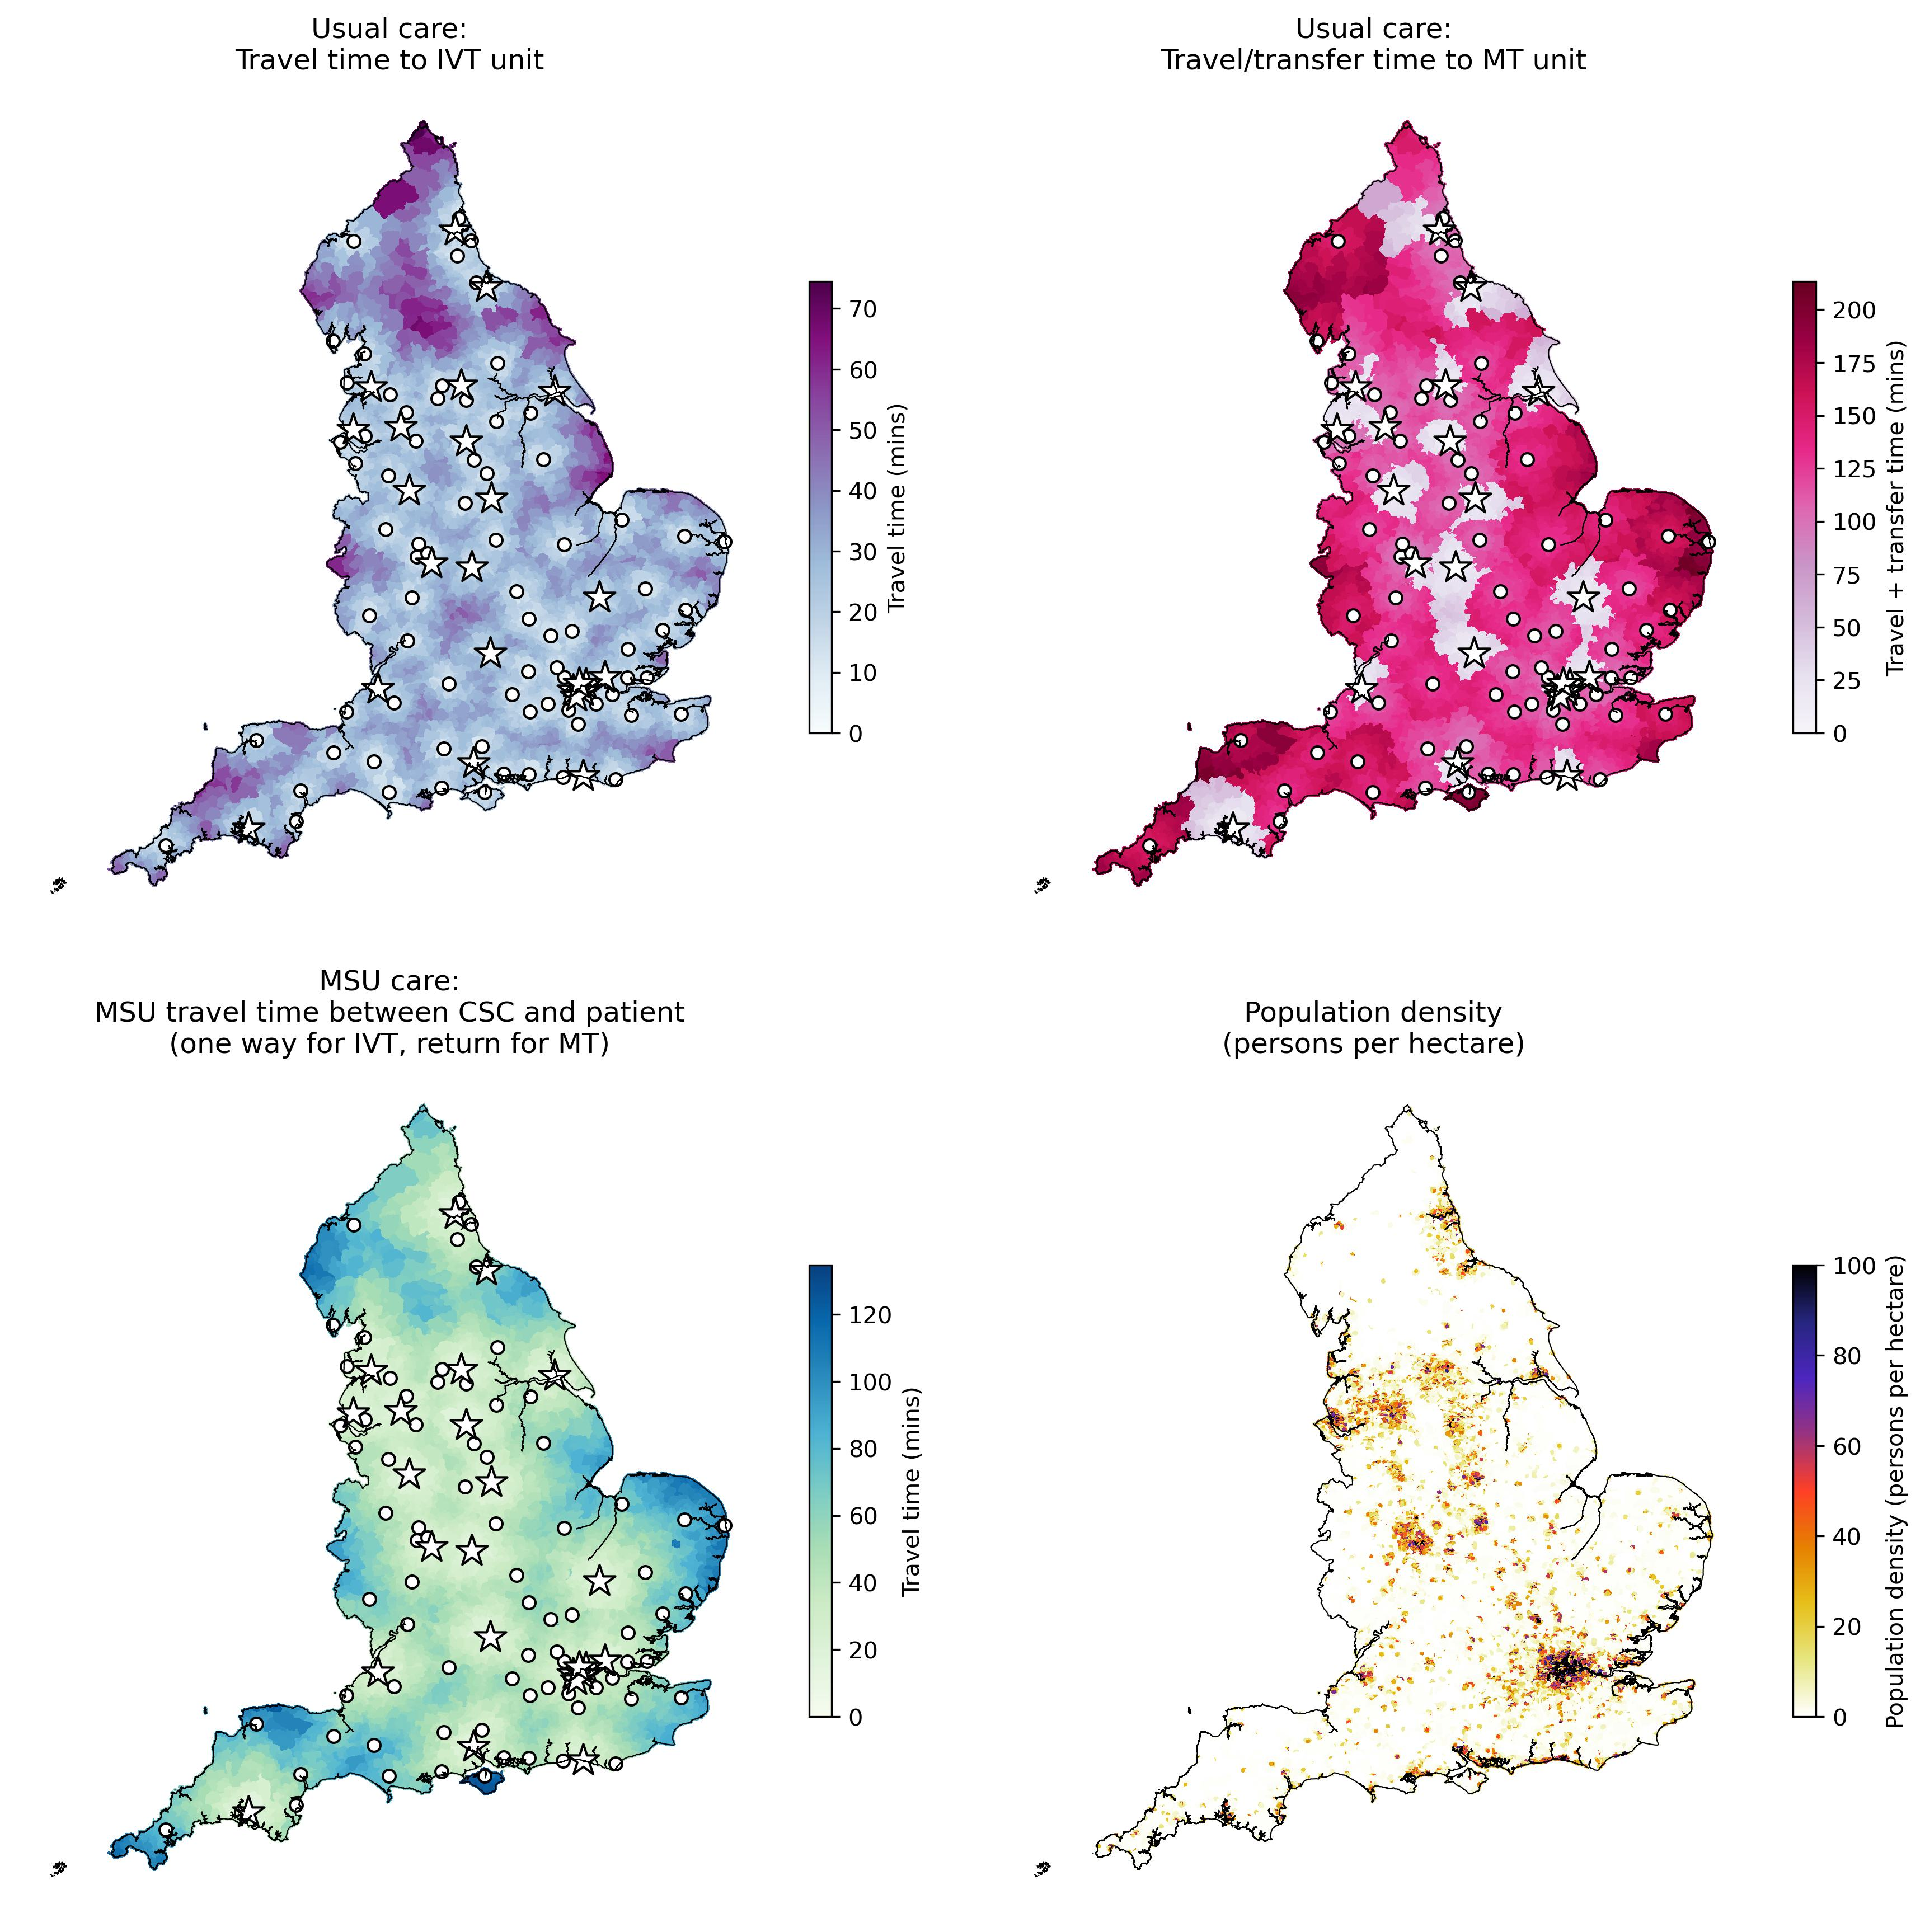
\includegraphics[width=1.0\linewidth]{images/map_times.jpg}
    \caption{Travel times to treatment under the two treatment delivery models, and population density for each LSOA. \textit{Top left}: With \emph{usual care} the travel times from the patients LSOA to their nearest PSC (providing only IVT). \textit{Top right}: With \emph{usual care} the travel and, where necessary, transfer times from the patients LSOA to a CSC (providing MT). For those patients that first attend a PSC providing only IVT, the times shown include the travel time to the PSC, a net additional delay of 60 minutes, and the inter-hospital travel time between PSC and CSC. \textit{Bottom left}: With \emph{MSU care} with the MSU base locations at the current 23 CSCs, the travel times for the MSU between the patients LSOA and their nearest CSC (one way for travel time to IVT, return journey for travel time to MT). \textit{Bottom right}: Population density (with scale capped at 100 persons per hectare). Circles show locations of PSCs (providing only IVT). Stars show locations of CSCs (providing both IVT and MT), and being the base locations of MSUs.}
    \label{fig:map_times}
\end{figure}

\begin{figure}[h!]
    \centering
    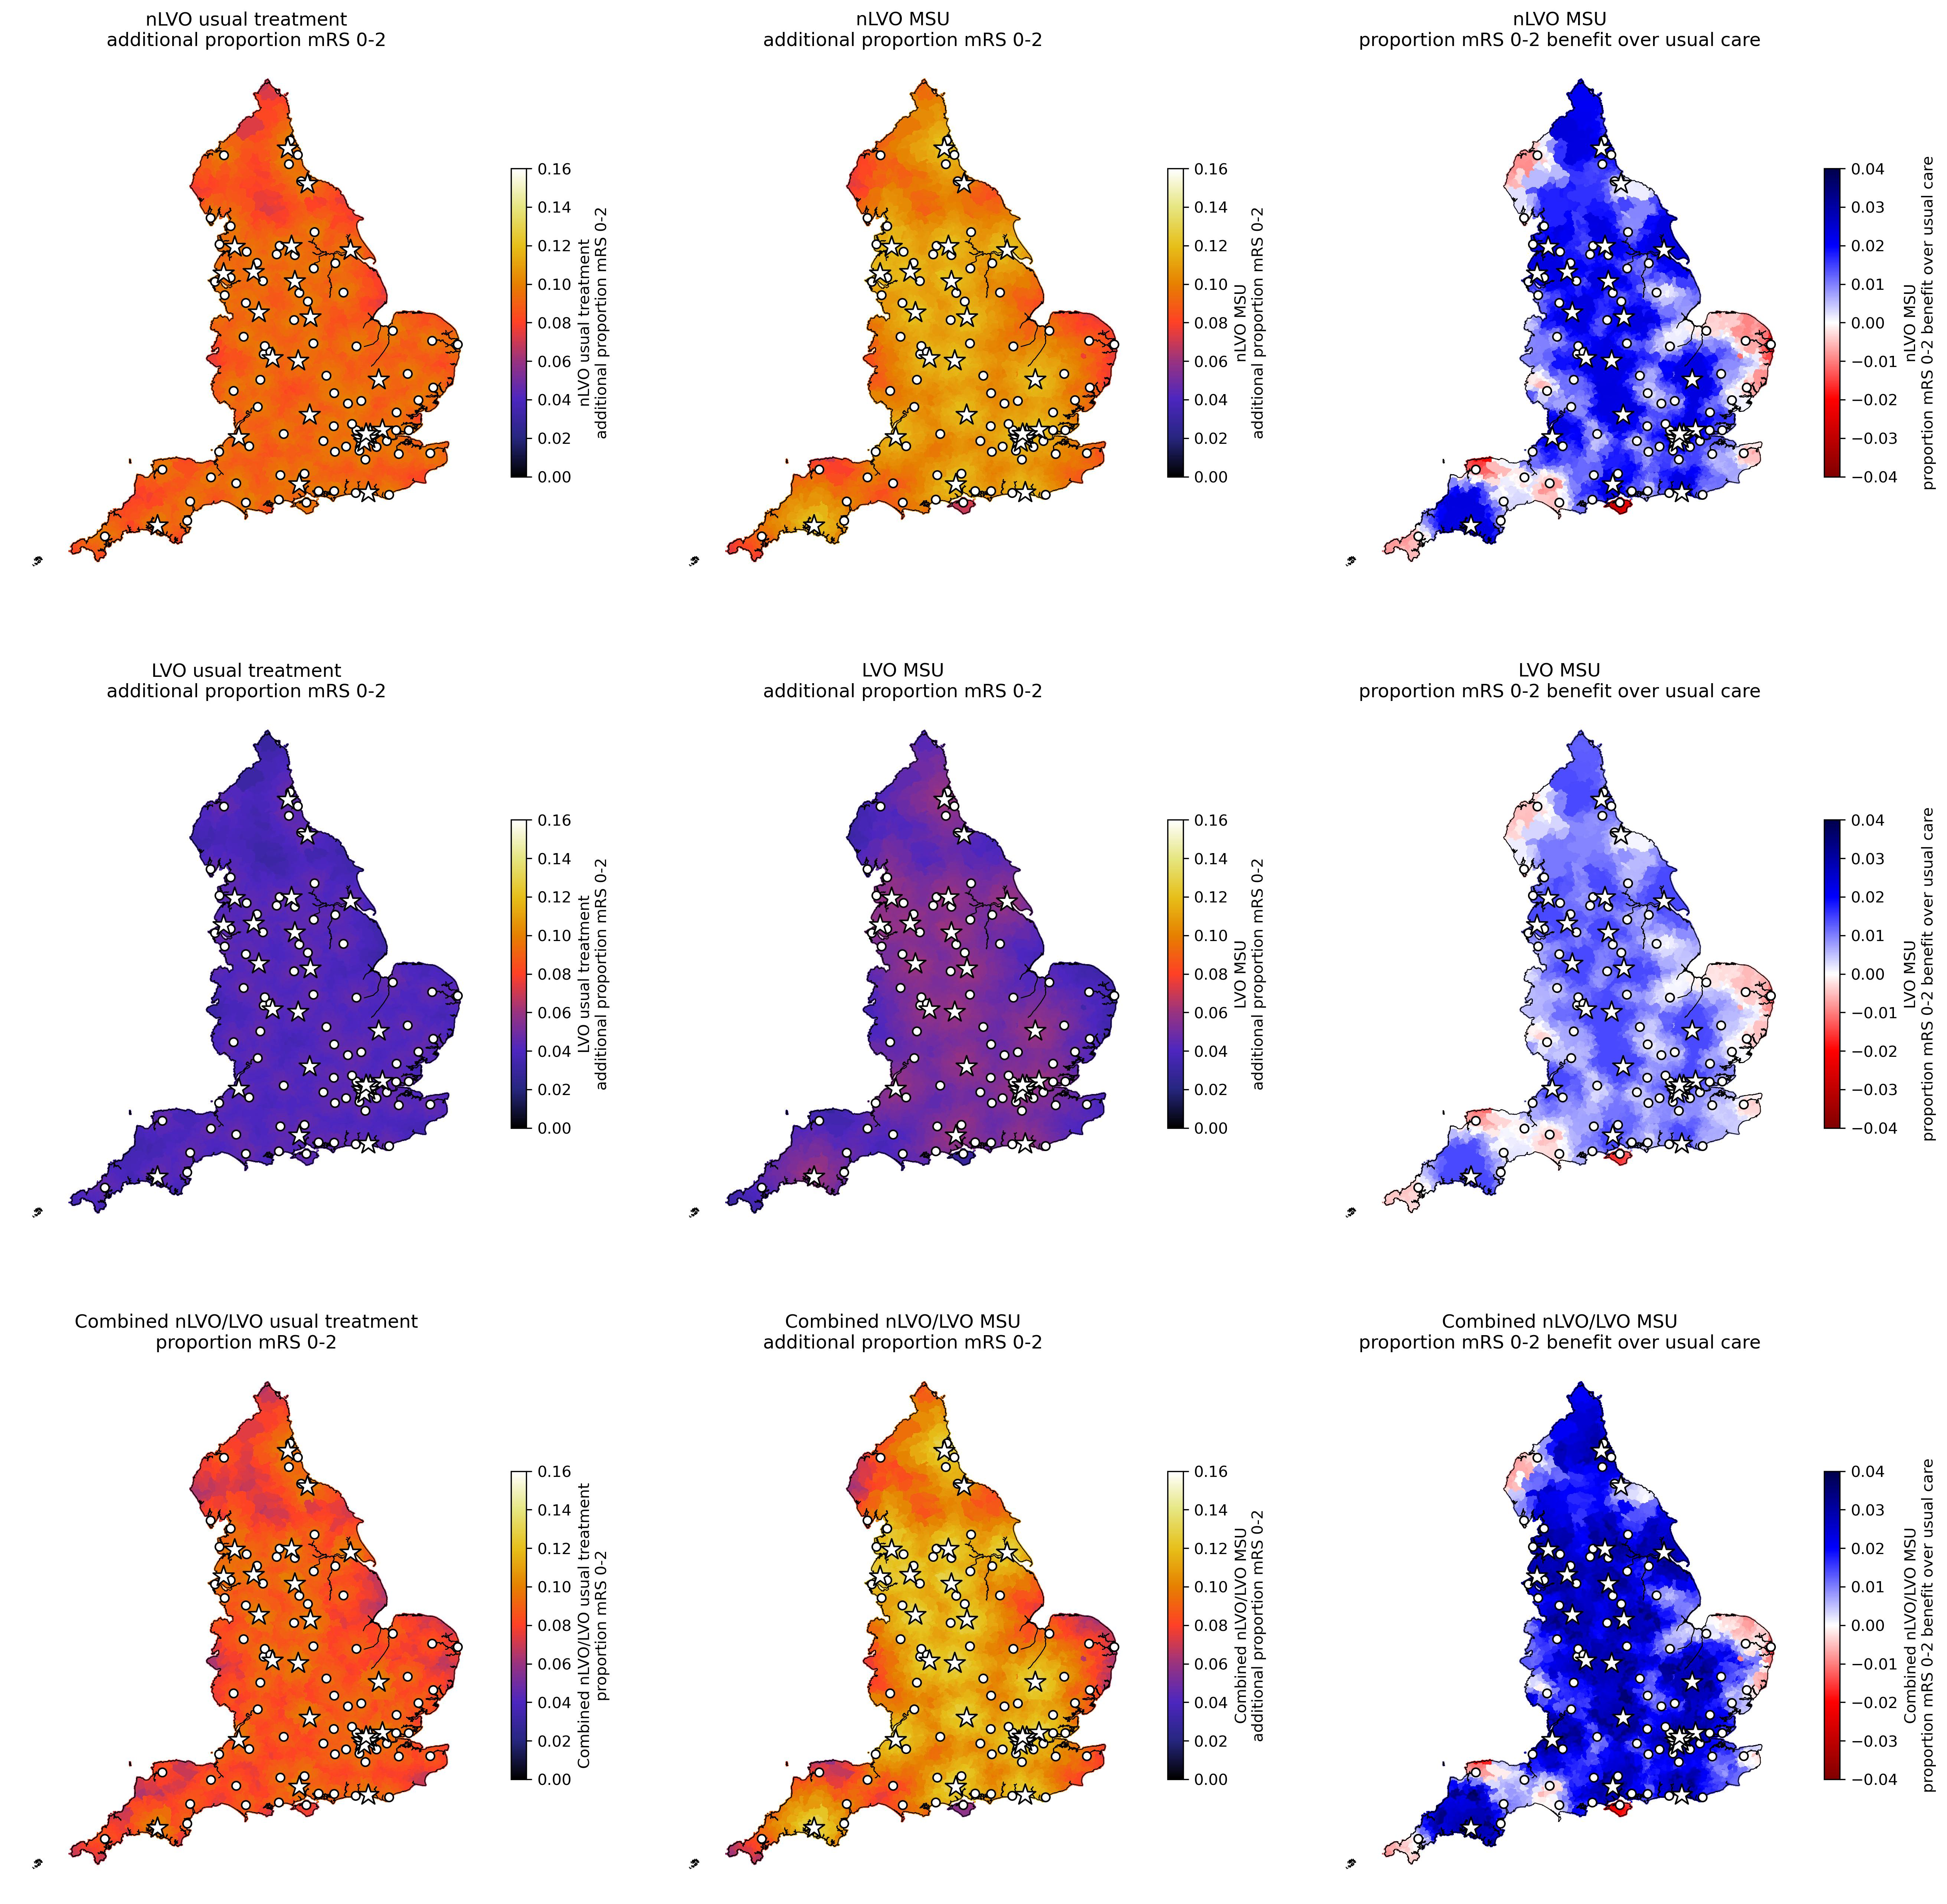
\includegraphics[width=1\linewidth]{images/map_mrs_0_2.jpg}
    \caption{Map of treatment benefits expressed as the proportion of patients with an outcome of mRS 0-2, calculated by LSOA for the treated population. \textit{Top}: Treatment of nLVO; \textit{Middle}: Treatment of LVO, \textit{Bottom}: Combination of treatment (based on 70\% nLVO and 30\% LVO in the treated population, with LVO receiving IVT/MT in combination). \textit{Left}: Benefit of usual care over no treatment; \textit{Middle}: Benefit of MSU care over no treatment; \textit{Right}: Benefit of MSU care over usual care. Circles show locations of PSCs (providing only IVT). Stars show locations of CSCs (providing both IVT and MT, and are also the base locations of MSUs).}
    \label{fig:msu_map_mrs_0_2}
\end{figure}

\begin{figure}[h!]
    \centering
    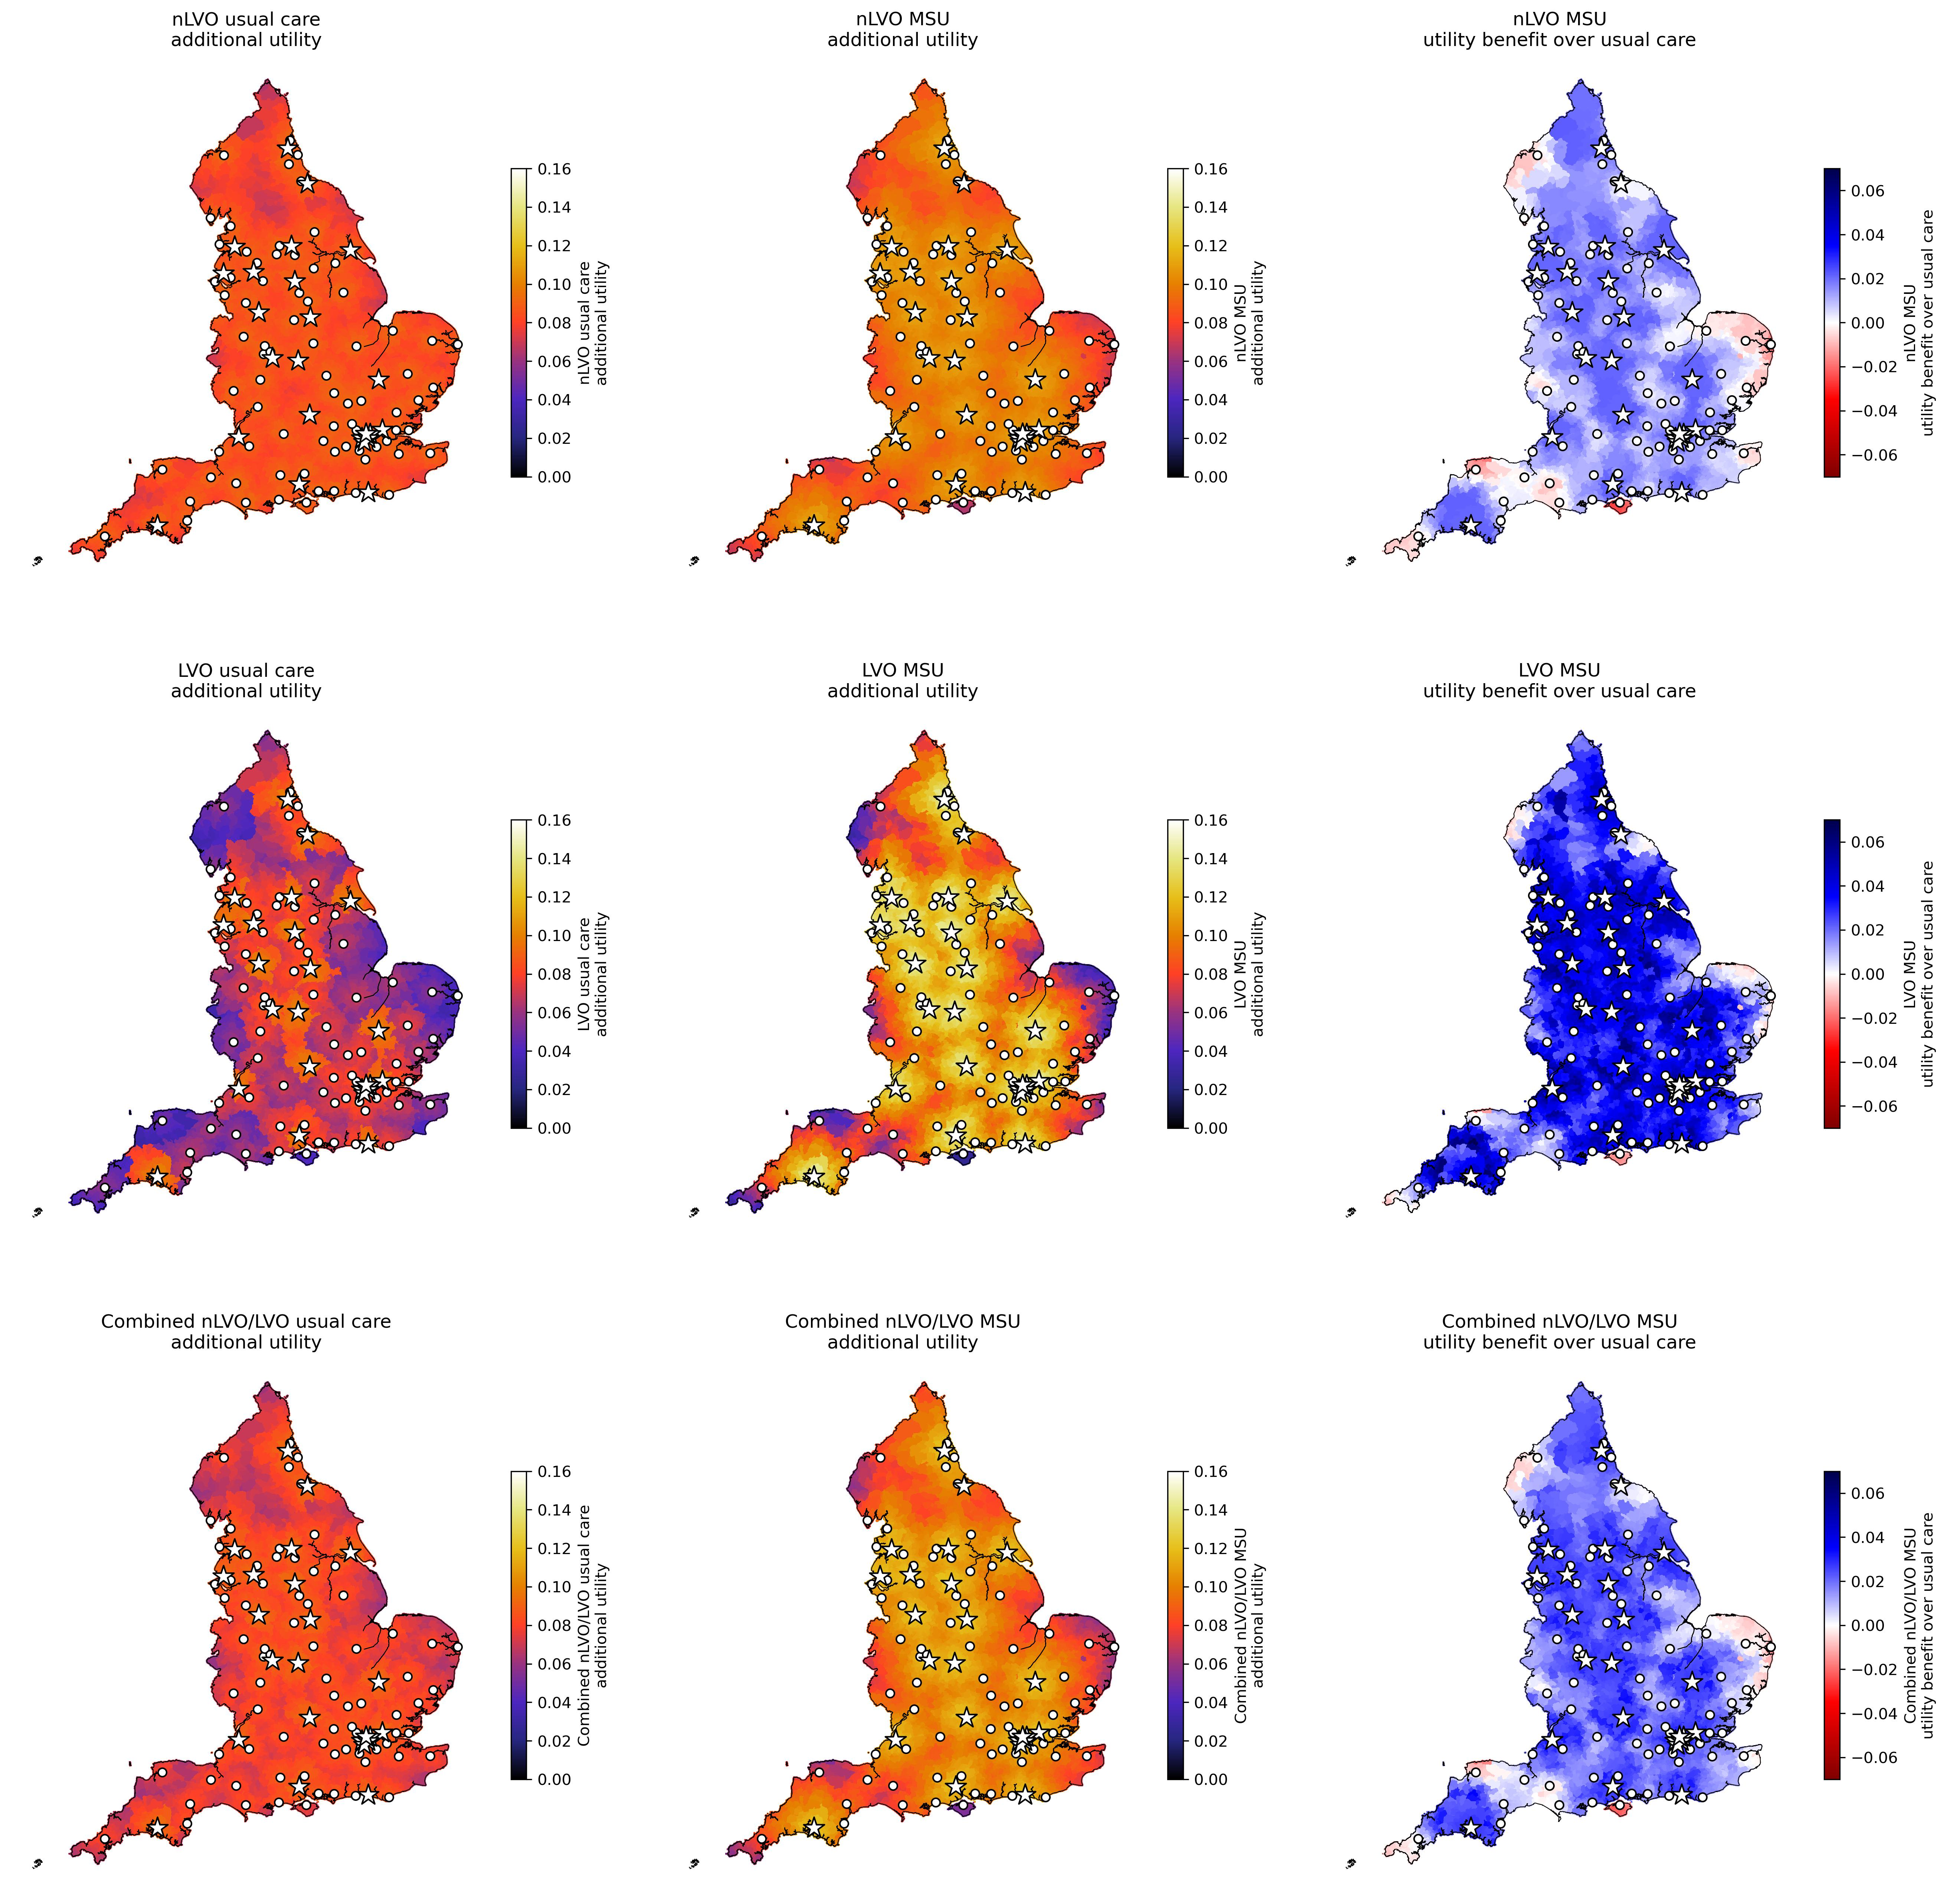
\includegraphics[width=1\linewidth]{images/map_utility.jpg}
    \caption{Map of treatment benefits expressed as the  utility benefit, calculated by LSOA for the treated population. \textit{Top}: Treatment of nLVO; \textit{Middle}: Treatment of LVO, \textit{Bottom}: Combination of treatment (based on 70\% nLVO and 30\% LVO in the treated population, with LVO receiving IVT/MT in combination). \textit{Left}: Benefit of usual care over no treatment; \textit{Middle}: Benefit of MSU care over no treatment; \textit{Right}: Benefit of MSU care over usual care. Circles show locations of PSCs (providing only IVT). Stars show locations of CSCs (providing both IVT and MT, and are also the base locations of MSUs).}
    \label{fig:msu_map_utility}
\end{figure}

\begin{figure}[h]
    \centering
    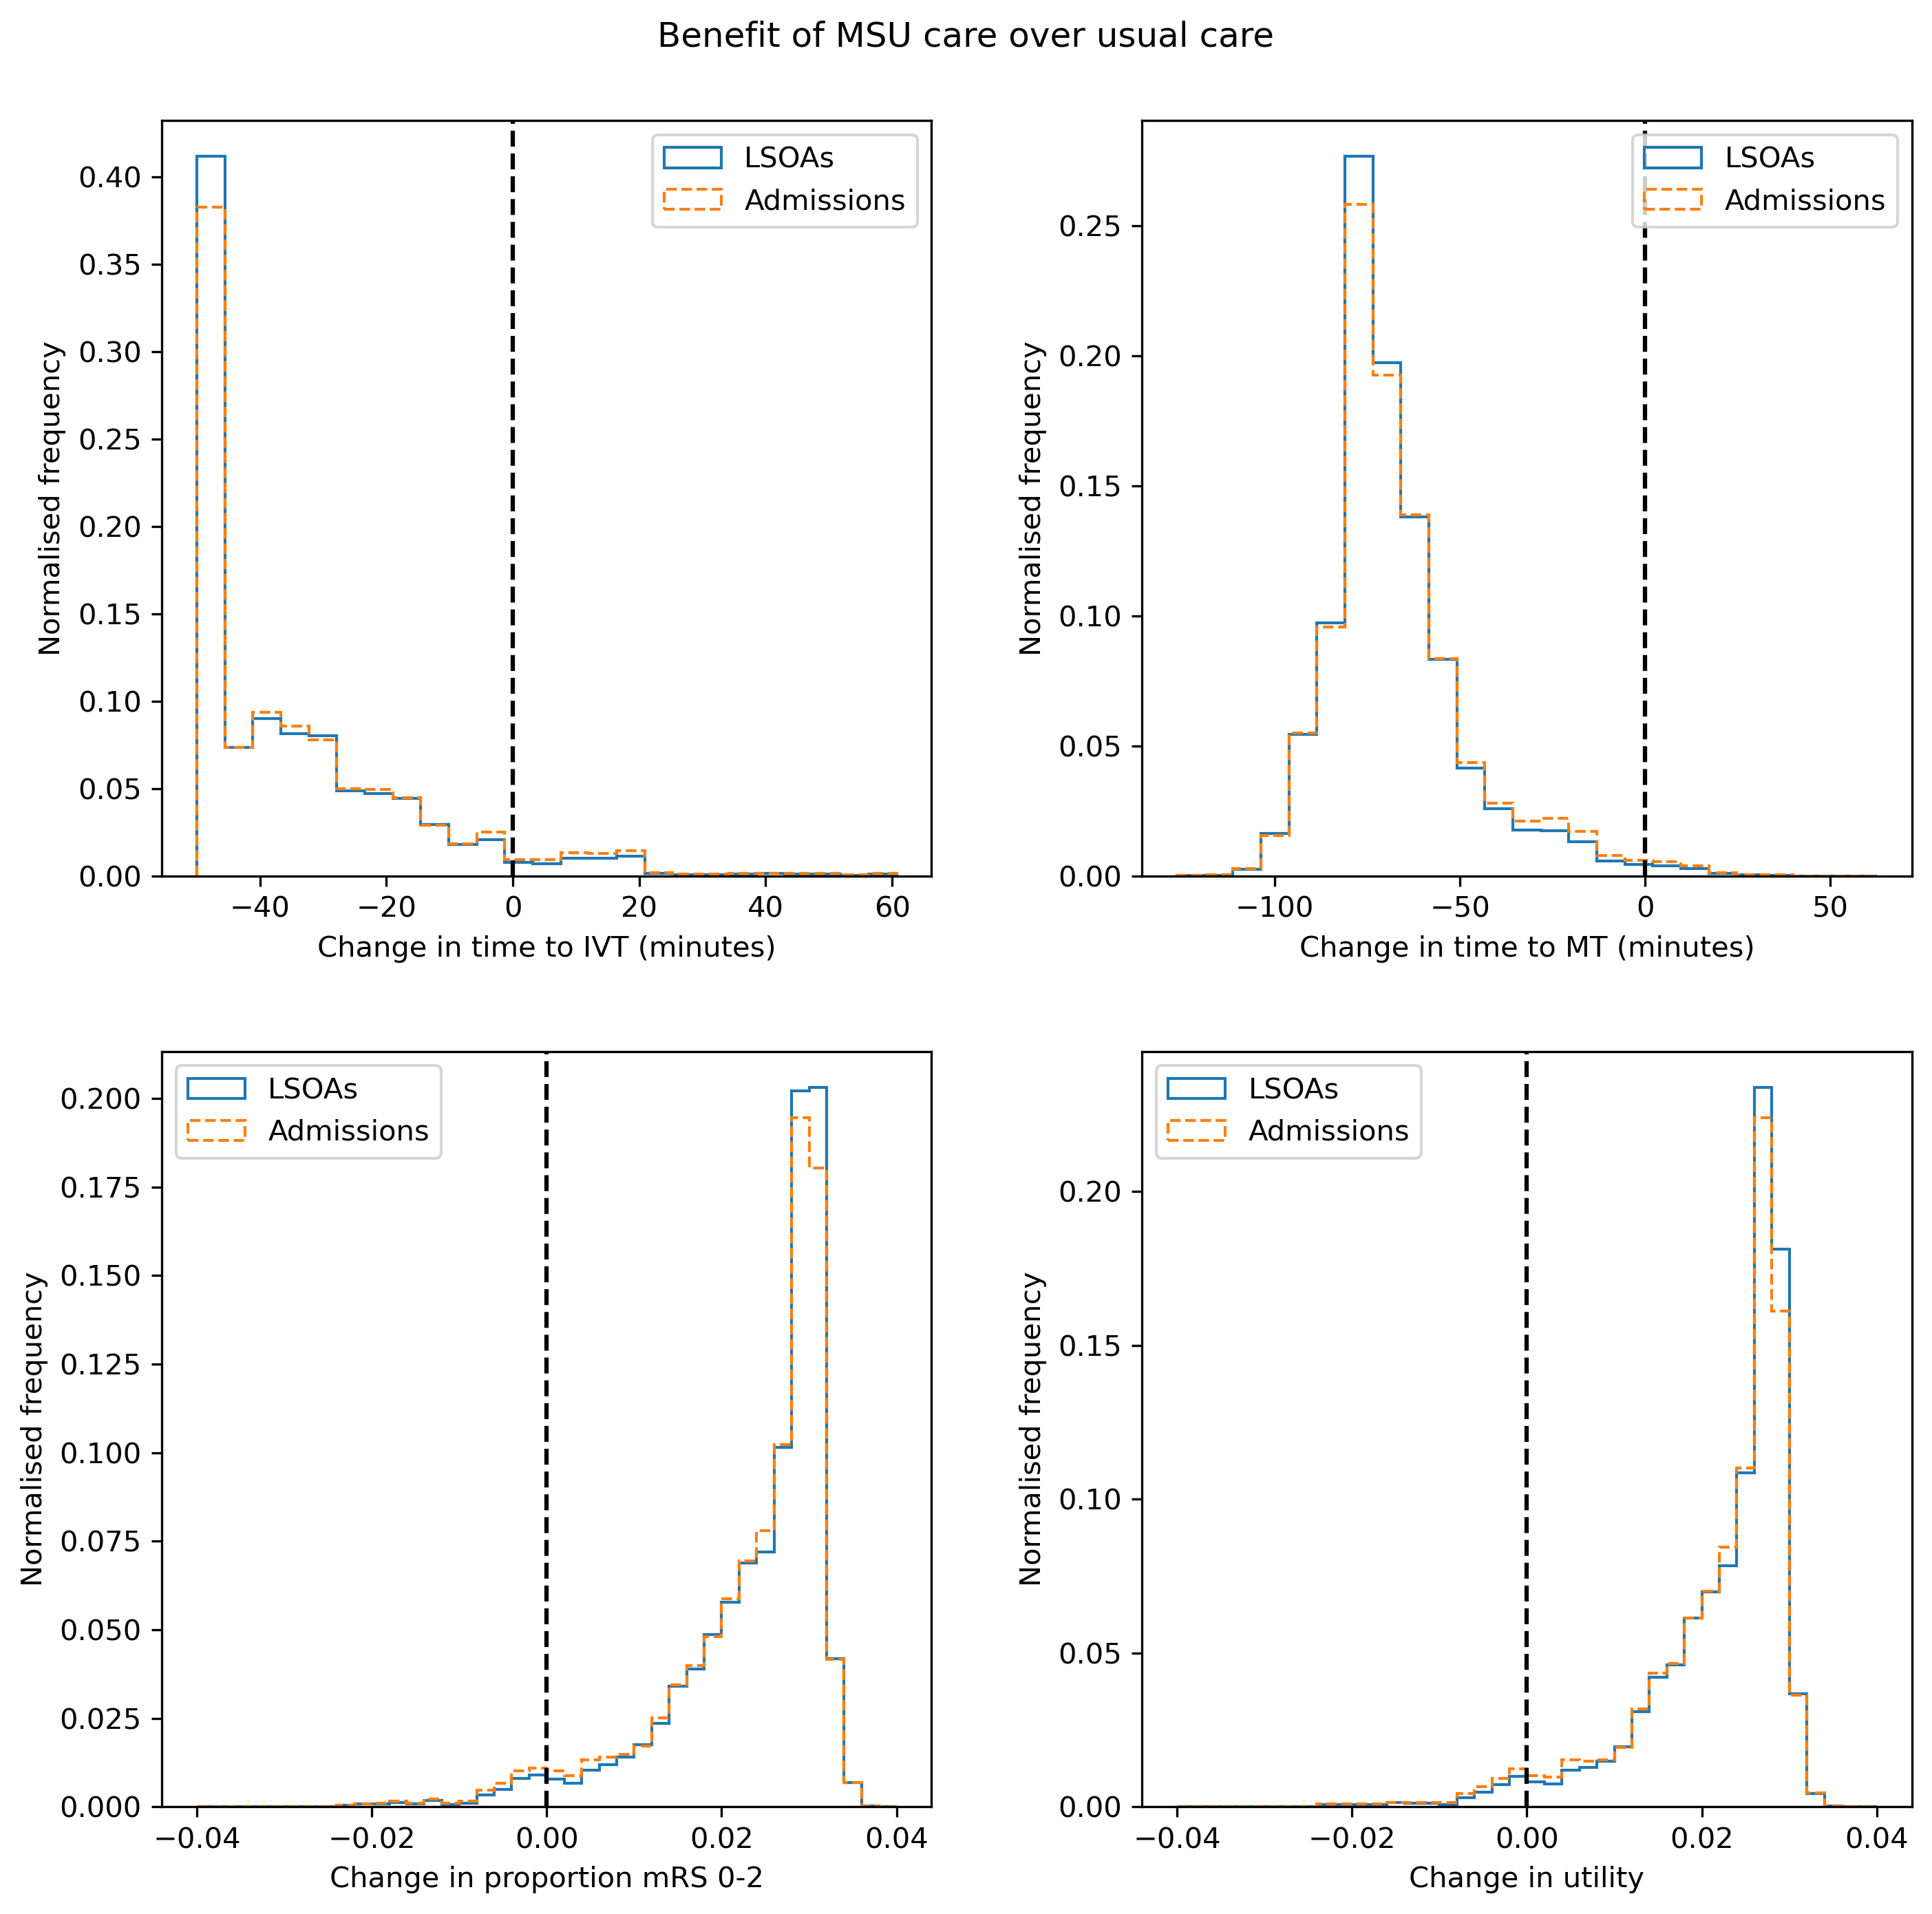
\includegraphics[width=0.75\linewidth]{images/histograms.png}
    \caption{Distribution of benefit of MSU care over usual care across LSOAs (assuming 70\% nLVO, 30\% LVO in the treated population, with LVO receiving IVT/MT in combination). Benefit is described either as even across LSOAs (solid line), or weighted by admissions by LSOA (dotted line). Histograms show change in time to IVT (top left), time to MT (top right), proportion mRS 0-2 post stroke (bottom left), or utility (bottom right).}
    \label{fig:msu_histograms}
\end{figure}

\begin{figure}[h]
    \centering
    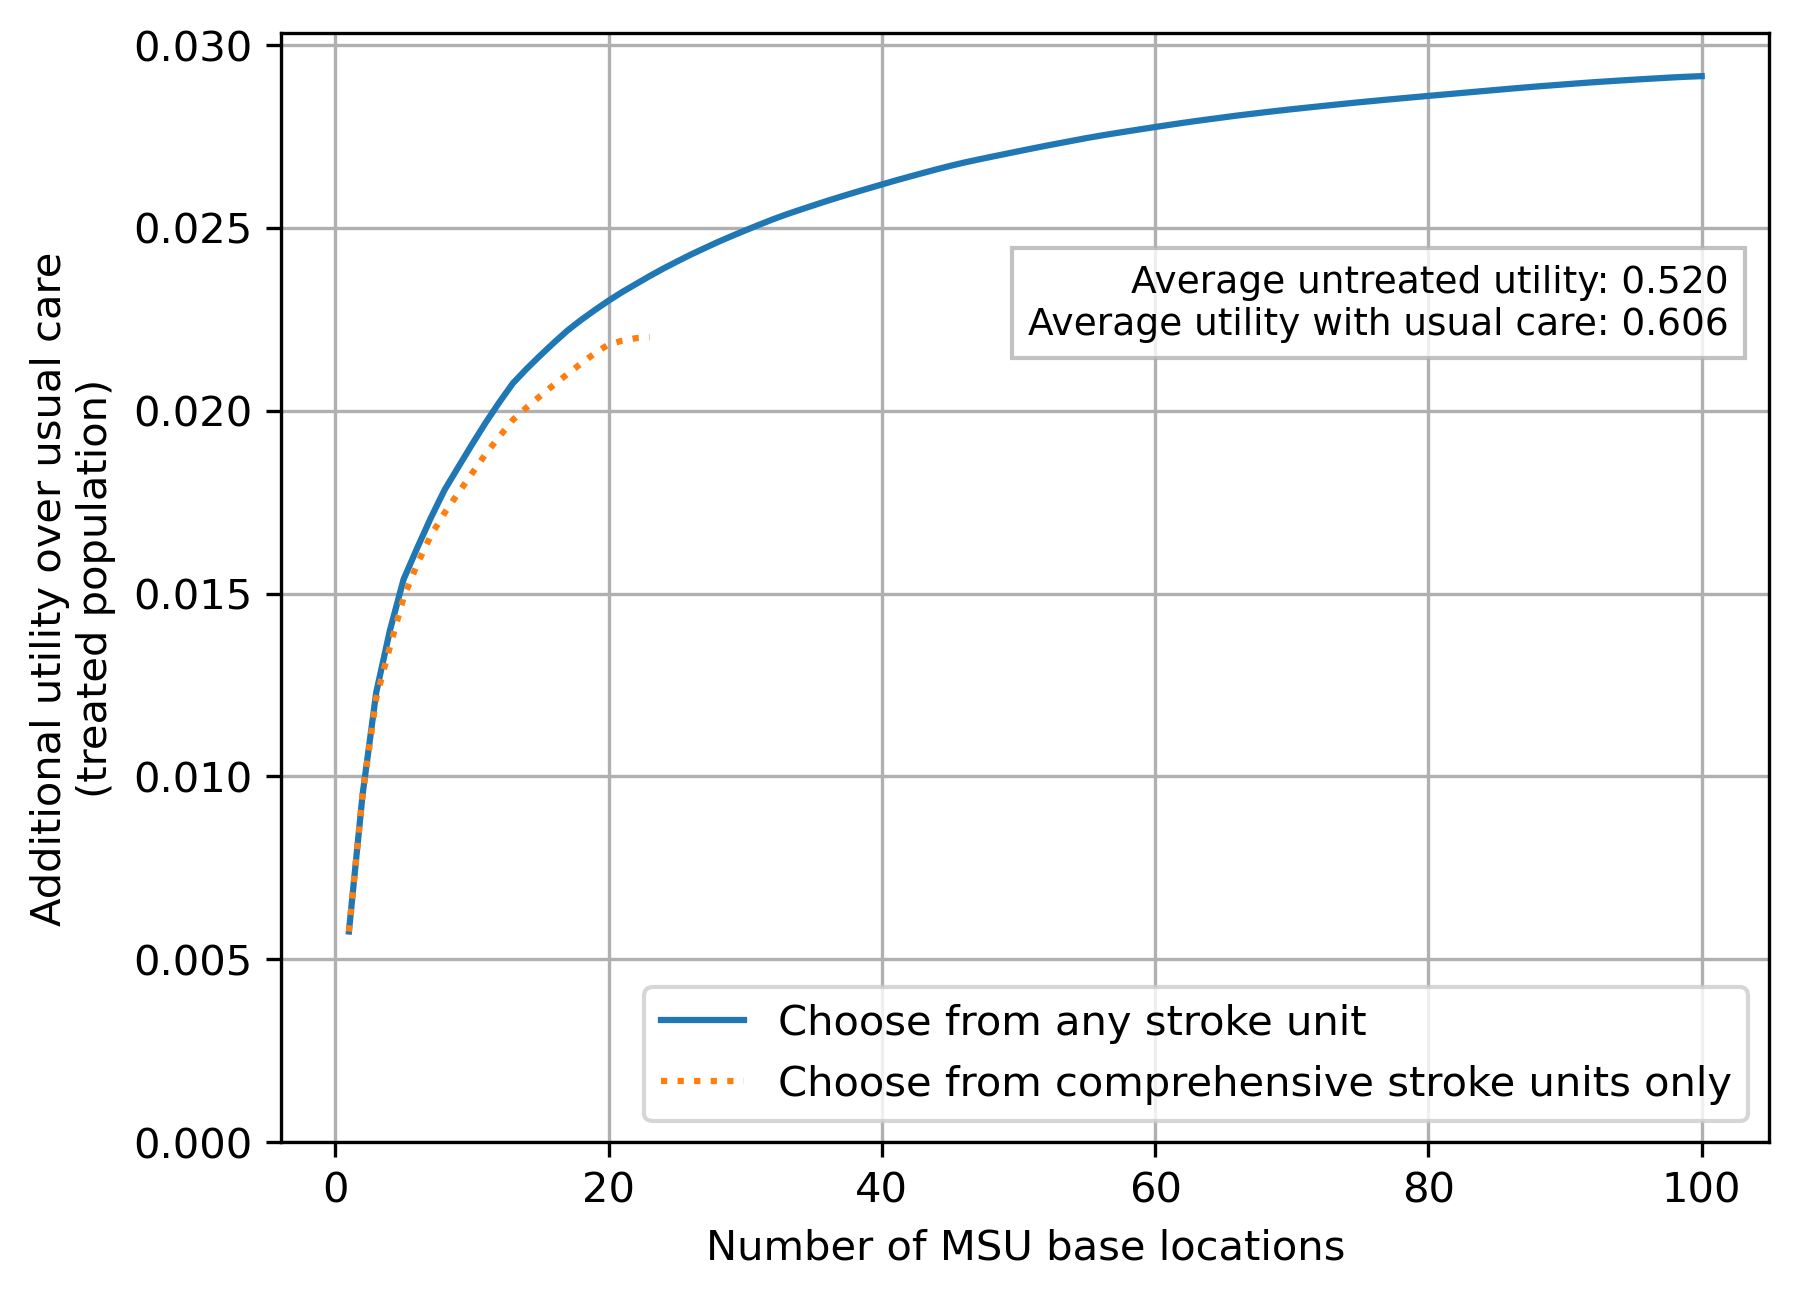
\includegraphics[width=0.5\linewidth]{images/msu_advantages_greedy.png}
    \caption{Increasing number of MSU base locations, with selection by a greedy algorithm based on improvements in utility. The additional utility is for those patients treated by MSU rather than usual care. Units were chosen either from any stroke centre type (solid line) or only from CSCs (dashed line). Utility for the untreated population was 0.520, which was increased to 0.602 with usual care.}
    \label{fig:greedy}
\end{figure}

% Number for supplementary material
\newcommand{\beginsupplement}{
    \setcounter{section}{0}
    \renewcommand{\thesection}{S\arabic{section}}
    \setcounter{figure}{0}
    \renewcommand{\thefigure}{S\arabic{figure}}
    \setcounter{table}{0}
    \renewcommand{\thetable}{S\arabic{table}}

}
%\clearpage
%\newpage
\begin{refsection} % Start referencing again for appendix
\beginsupplement
%TC:igno
\appendix
%%%%%%%%%%%%%% Change all tenses to past tesse

\section{Outcome modelling}

\subsection{Modified Rankin scale}

We used modified Rankin Scale (mRS) at 6 months as a measure of outcome. mRS is the instrument most commonly used to describe the functional outcome post-stroke \cite{quinn_functional_2009}, describing the independence of living on a scale of 0 (no disability) to 5 (severe disability requiring constant nursing attention), with death assigned an mRS of 6. A commonly used surrogate for independent living is mRS 0-2. The health utility values for each mRS level were taken from Wang \textit{et al.} \cite{wang_utility-weighted_2020}. These were 0.0, -0.19, 0.20, 0.55, 0.74, 0.88 and 0.97 for mRS 0-6. The mean mRS score, the mean utility, and the proportion of patients with mRS 0-2 in a given mRS distribution can be compared between scenarios. Table \ref{tab:mrs} shows a description of each mRS category.

\begin{minipage}{1.0\textwidth}  % Define the width of the minipage
\begin{longtable}{p{1.2cm} p{13cm}}
\caption{Description of modified Rankin Scale (mRS)categories}\label{tab:mrs}\\
\toprule
mRS & Description \\
\midrule
0 & No symptoms. \\
1 & No significant disability. Able to carry out all usual activities, despite some symptoms.\\
2 & Slight disability. Able to look after own affairs without assistance but unable to carry out all previous activities. \\
3 & Moderate disability. Requires some help, but able to walk unassisted.\\
4 & Moderately severe disability. Unable to attend to their own bodily needs without assistance and unable to walk unassisted. \\
5 & Severe disability. Requires constant nursing care and attention,
bedridden, incontinent.\\
6 & Dead.\\
\bottomrule
\end{longtable}
\end{minipage} 


\subsection{Treatment of ischaemic stroke}

Reperfusion treatment aims to restore blood flow after an ischaemic stroke. There are two potential reperfusion treatments:

\begin{itemize}
    \item \textit{Thrombolysis} (also known as intravenous thrombolysis, IVT) is a medical therapy in which clot-busting drugs are used to reduce or remove the blood clot. It is potentially of use in both nLVO and LVO.
    
    \item \textit{Thrombectomy} (also known as mechanical thrombectomy, MT) is the physical removal of a clot, by a mesh device under image guidance. Thrombectomy is suitable only for clots in a large vessel (these generally cause the worst strokes). It is potentially of use in LVO.
\end{itemize}


\subsection{Outcome modelling overview}

Detailed methods and code used for modelling these outcomes are available \cite{github2}, with methods described as an online book \cite{github3}. The outcome model is available as a PyPI package for Python \cite{pypi}.

We used modified Rankin Scale (mRS) at 3-6 months as a measure of outcome. mRS is the most commonly used instrument to describe post-stroke functional outcome \cite{quinn_functional_2009}, describing independence of living from a scale of 0 (no disability) through to 5 (severe disability requiring constant nursing attention), with death assigned an mRS of 6. A commonly used surrogate for independent living is  mRS 0-2. Health utility values for each mRS level were taken from Wang \textit{et al.} \cite{wang_utility-weighted_2020}. The mean mRS score, mean utility and proportion of patients with mRS 0-2 in a given mRS distribution can be compared between scenarios.

We calculated the patients mRS outcome distribution based on time to treatment for three patient-treatment cohorts: nLVO treated with IVT; LVO treated with IVT alone; and LVO treated with IVT and MT. For each patient-treatment cohort we calculated an mRS distribution for treatment at any given time by interpolating between the mRS distribution for treatment given at \emph{t=0} (time of stroke onset) and the mRS distribution for treatment given at \emph{t=No Effect} (time of no effect of treatment), assuming that log odds fall linearly over time \cite{emberson_effect_2014, fransen_time_2016}.

The time to no effect was 6.3 hours for IVT \cite{emberson_effect_2014} and 8.0 hours for MT \cite{ fransen_time_2016}. Our model did not include selection of patients who may still benefit from treatment beyond these durations through the use of perfusion scanning. This number is small for IVT, but is more substantial for MT – approximately 2,500 per annum in England. 

The model synthesises data from multiple sources (figure \ref{fig:data_cauldron}) including reperfusion treatment clinical trials and national stroke audit data for England and Wales. Predictions from the combined model are then compared against original clinical trials and other models. Details of how these data are synthesised are given in the sections below.

\begin{figure}[h!]
    \centering
    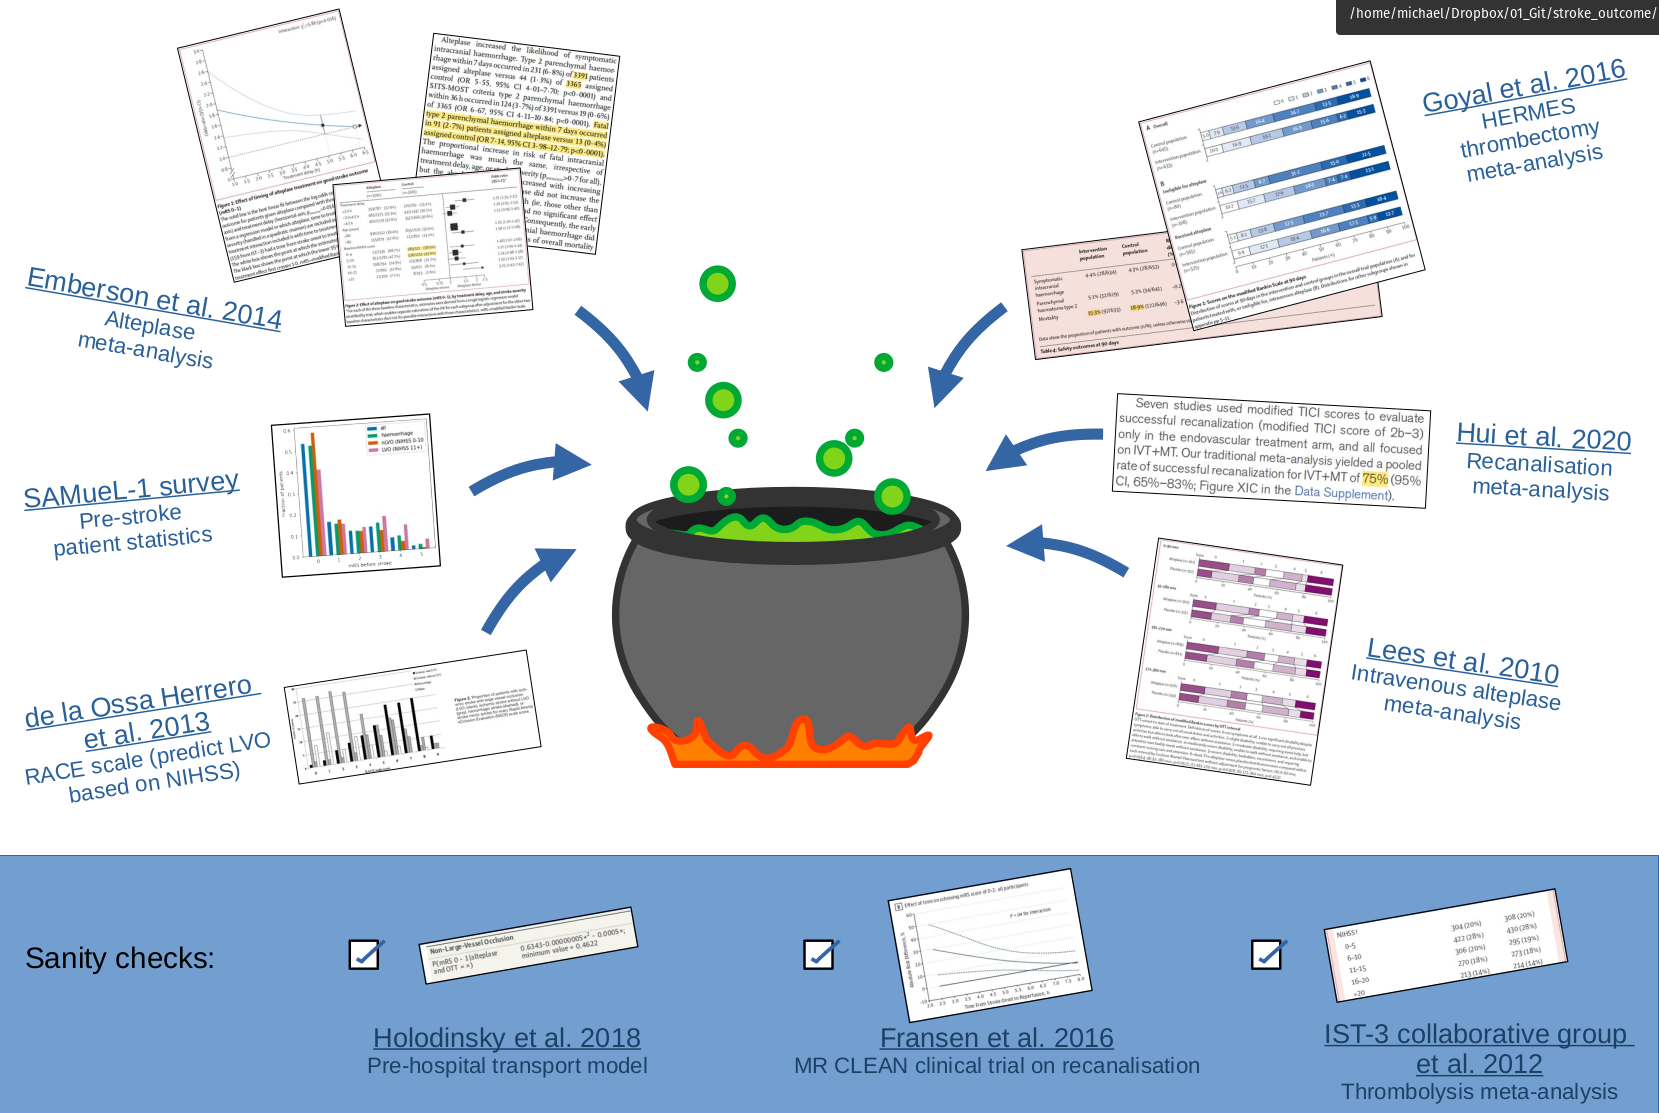
\includegraphics[width=1.0\linewidth]{images_modelling/data_cauldron.png}
    \caption{Depiction of hoe multiple data sources are combined to produce a mRS-level outcome model of nLVO and LVO stroke treated with thrombolysis and/or thrombectomy.}
    \label{fig:data_cauldron}
\end{figure}

The model results in mRS probability distributions for nLVO treated with IVT and LVO treated with IVT or MT (Figure \ref{fig:probs_with_time}).

\begin{figure}[h!]
    \centering
    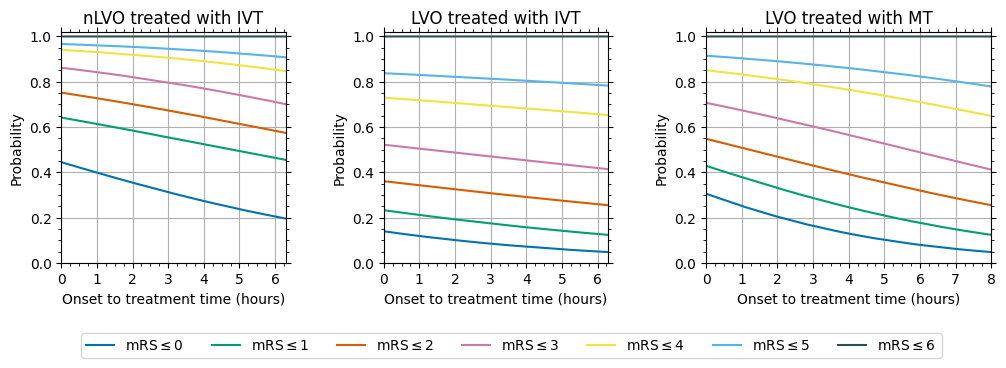
\includegraphics[width=1.0\linewidth]{images_modelling/probs_with_time.png}
    \caption{Final model predictions of mRS distributions for nLVO and LVO depending on time to treatment with IVT (for nLVO or LVO) or thrombectomy (for IVT and LVO).}
    \label{fig:probs_with_time}
\end{figure}

\subsection{Extrapolation of reperfusion effects back to time zero}

In order to model the effectiveness of reperfusion at any given time point, we interpolate between the theoretical effectiveness at time zero (the time of stroke onset) and the time at which the treatment no longer has any efficacy (the time of no effect). Clinical trials model this decay as a linear decay on log odds of improved outcome \cite{emberson_effect_2014, fransen_time_2016}. An illustration of how this was done is shown in figure \ref{fig:decay}.

\begin{figure}[h!]
    \centering
    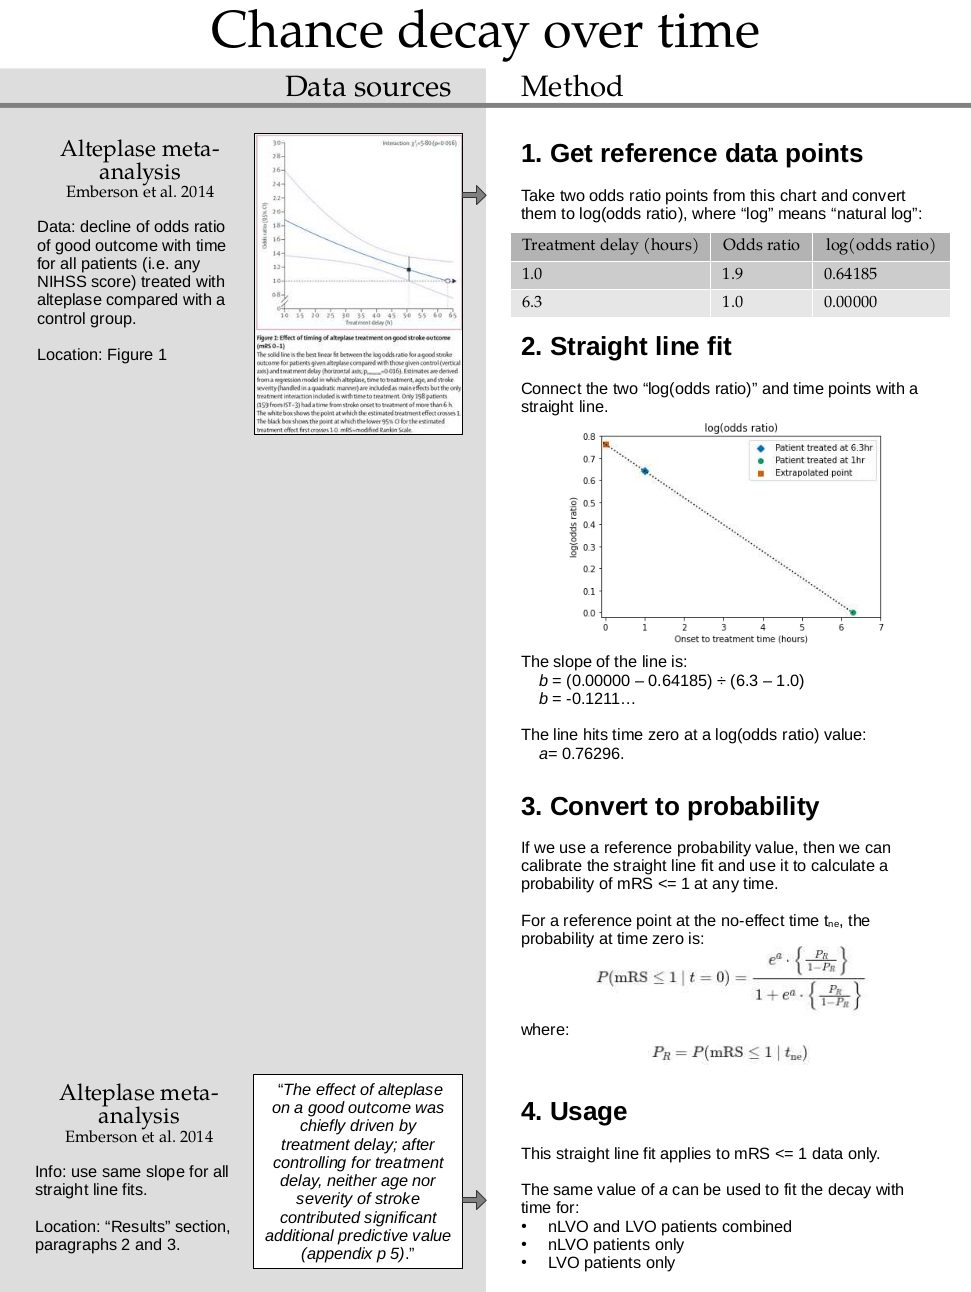
\includegraphics[width=1.0\linewidth]{images_modelling/data_sources_decay.png}
    \caption{Extrapolation of clinical trial results back to time zero, the time of onset of stroke}
    \label{fig:decay}
\end{figure}

\subsection{Derivation of mRS distributions from reference data}

\subsubsection{Plain English summary}

When we predict the outcome of a person who has had a stroke, we want to be able to say what is the likely improvement in disability level they would experience due to the treatment.

The modified Rankin Scale is used to assign a level of disability to a patient who has had a stroke. When looking at the mRS scores of a whole population, some scores are more likely to occur than others depending on who is included in that population. The improvement in disability level they can get will depend on the time from when their stroke symptoms began and when they receive treatment. The best possible outcome would be if they were treated immediately after they had their stroke. The benefit of treatment reduces over time until the treatment no longer offers any benefit, and they will not be better off than having no treatment. We can look at the proportion of people with each mRS score as the \emph{probability} of having that mRS score.

The main aim of the stroke outcome model is to be able to predict the range of mRS scores of various different populations. We would like to know the expected mRS scores of groups of people before a stroke, people who received no treatment for their stroke, and people who were treated at any chosen time after their stroke began. There is no real-life data for this last group of people. However we can create a model that creates that data by combining other real-life datasets. The real-life datasets come from various clinical trials.

We assume that the mRS scores of people after stroke depend on their time to treatment. The more time that passes between the start of the stroke and the treatment, the more likely it is that people will have higher disability scores. This continues up until a \emph{time of no effect} where the patients cannot benefit from the treatment but still run the risks of death due to the treatment.

This document shows how to combine the real-life datasets to create mRS distributions that will be used everywhere in the stroke outcome model.

The final datasets will cover these three main groups of people:

\begin{itemize}
    \item Patients with a non-Large-Vessel Occlusion (nLVO) who were treated with intravenous thrombolysis (IVT).
    \item Patients with a Large-Vessel Occlusion (LVO) who were treated with intravenous thrombolysis (IVT).
    \item Patients with a Large-Vessel Occlusion (LVO) who were treated with mechanical thrombectomy (MT).
\end{itemize}

\subsubsection{General method}

The steps to create the mRS distributions are:

\begin{enumerate}
    \item Estimate the mRS distributions of populations before their stroke.
    \begin{itemize}
        \item These data are available in the SSNAP data.
        \item We split the full cohort of patients into nLVO and LVO based on their NIHSS score (using NIHSS 11+ as a surrogate indicator of a large vessel occlusion stroke).
    \end{itemize}
     \item Estimate the mRS distributions of populations that received no treatment.
    \begin{itemize}
        \item This data is available for two groups. The first group is patients with LVOs. The second group is a mix of patients with nLVOs and patients with LVOs.
        \item We combine the groups and infer the distribution for the population patients with nLVO (as nLVO-specific data is not available).
    \end{itemize}
        \item Estimate the mRS distributions of populations if they treated at the time of no beneficial effect.
    \begin{itemize}
        \item At the time of no effect, we assume that patients given the treatment will see no benefit but are still exposed to a risk of death from treatment.
    \item We take the distributions for populations that received no treatment and adjust them for this predicted death rate in the absence of a beneficial treatment effect.
    \end{itemize}
    \item Estimate the mRS distributions of populations if they were treated at time zero (the time of stroke).
    \begin{itemize}
        \item For IVT:
        \begin{itemize}
            \item We take reference data points for mRS $\leq$ 1 at time zero and the mRS distributions at the time of no effect. Plugging these into a formula for the changing probability of the mRS $\leq$ 1 score with time lets us find the probability distributions at time zero.
            \item Fixing this point, we take a weighted combination of the pre-stroke and no-effect distributions so that the combination's mRS $\leq$ point matches the fixed point.
        \end{itemize}     
    \end{itemize}
    \begin{itemize}
        \item For MT:
        \begin{itemize}
            \item Define the time-zero distribution as a weighted combination of 75\% of the pre-stroke distribution and 25\% of the no-effect distribution.
            \item Adjust the excess death rate until the mRS distribution at a reference data time matches the mortality rate at that reference time. 
        \end{itemize}
    \end{itemize}    
\end{enumerate}

Figure \ref{fig:data_sources_grid} shows a summary of the data sources used to estimate the mRS distribution for each reference population, with figure \ref{fig:data_sources_summary} showing flow of information and resulting distributions.

\begin{figure}[h!]
    \centering
    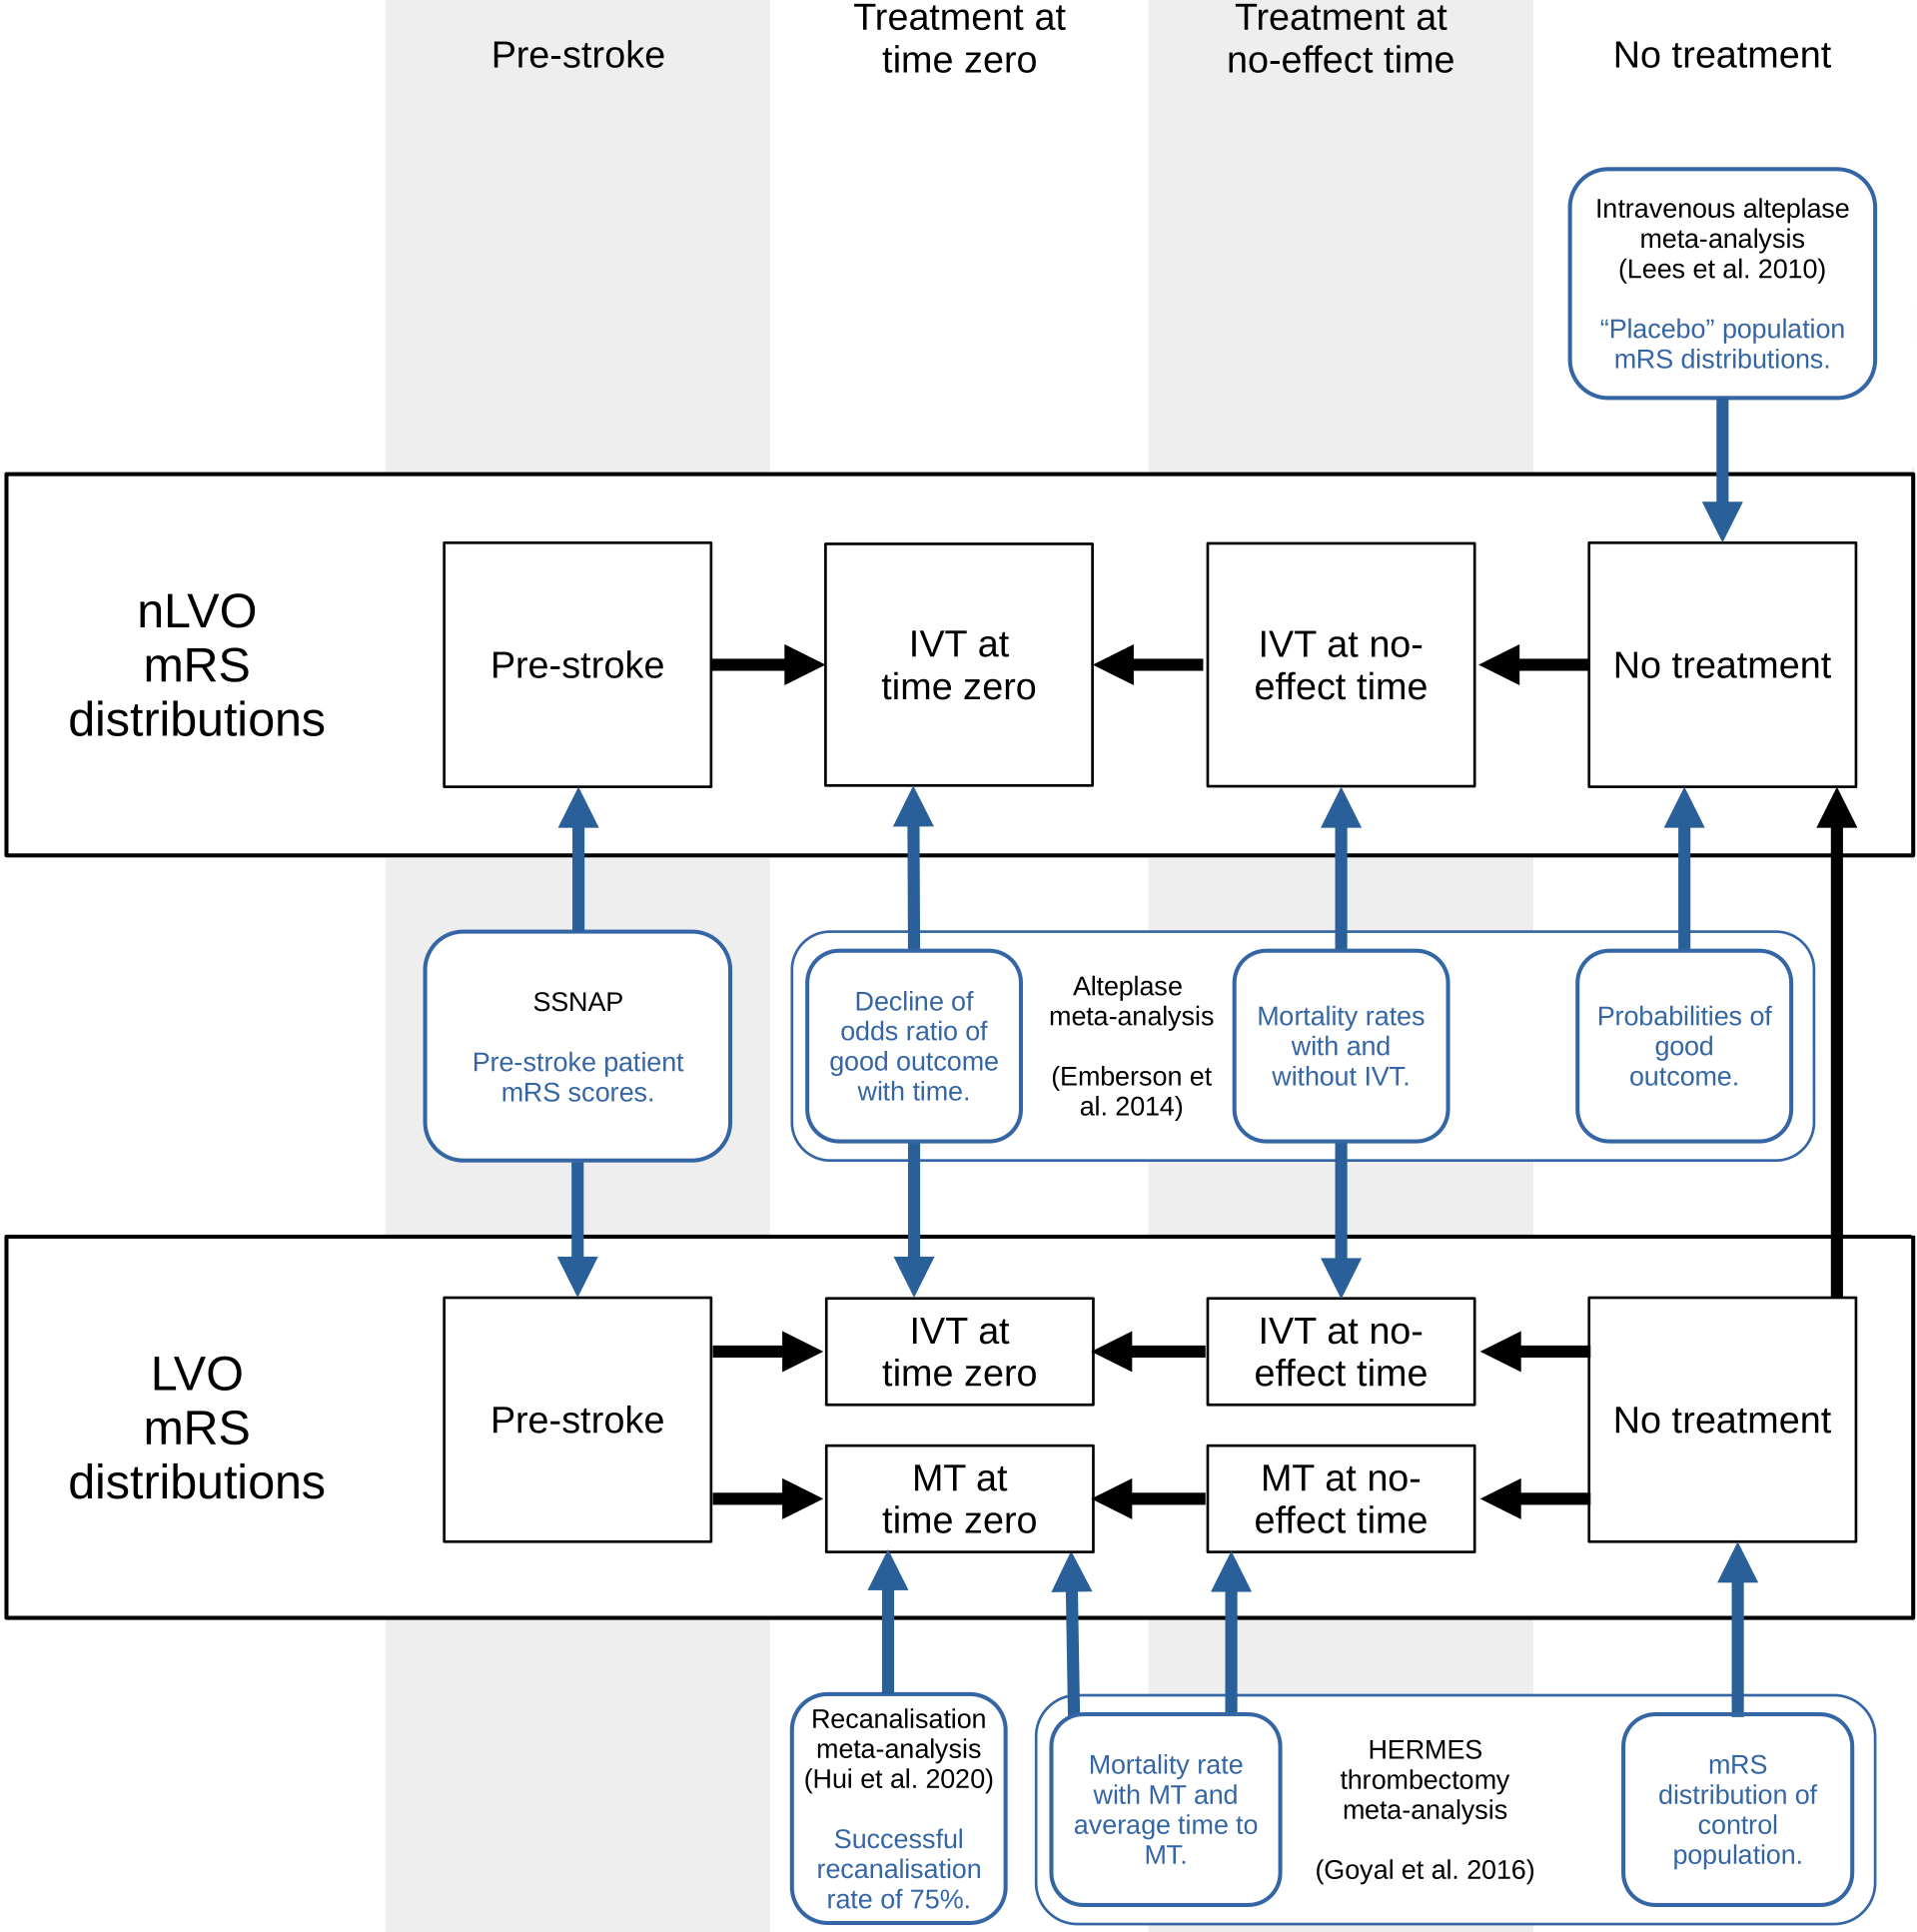
\includegraphics[width=1.0\linewidth]{images_modelling/data_sources.png}
    \caption{Summary of data sources used to estimate reference distributions.}
    \label{fig:data_sources_grid}
\end{figure}

\begin{figure}[h!]
    \centering
    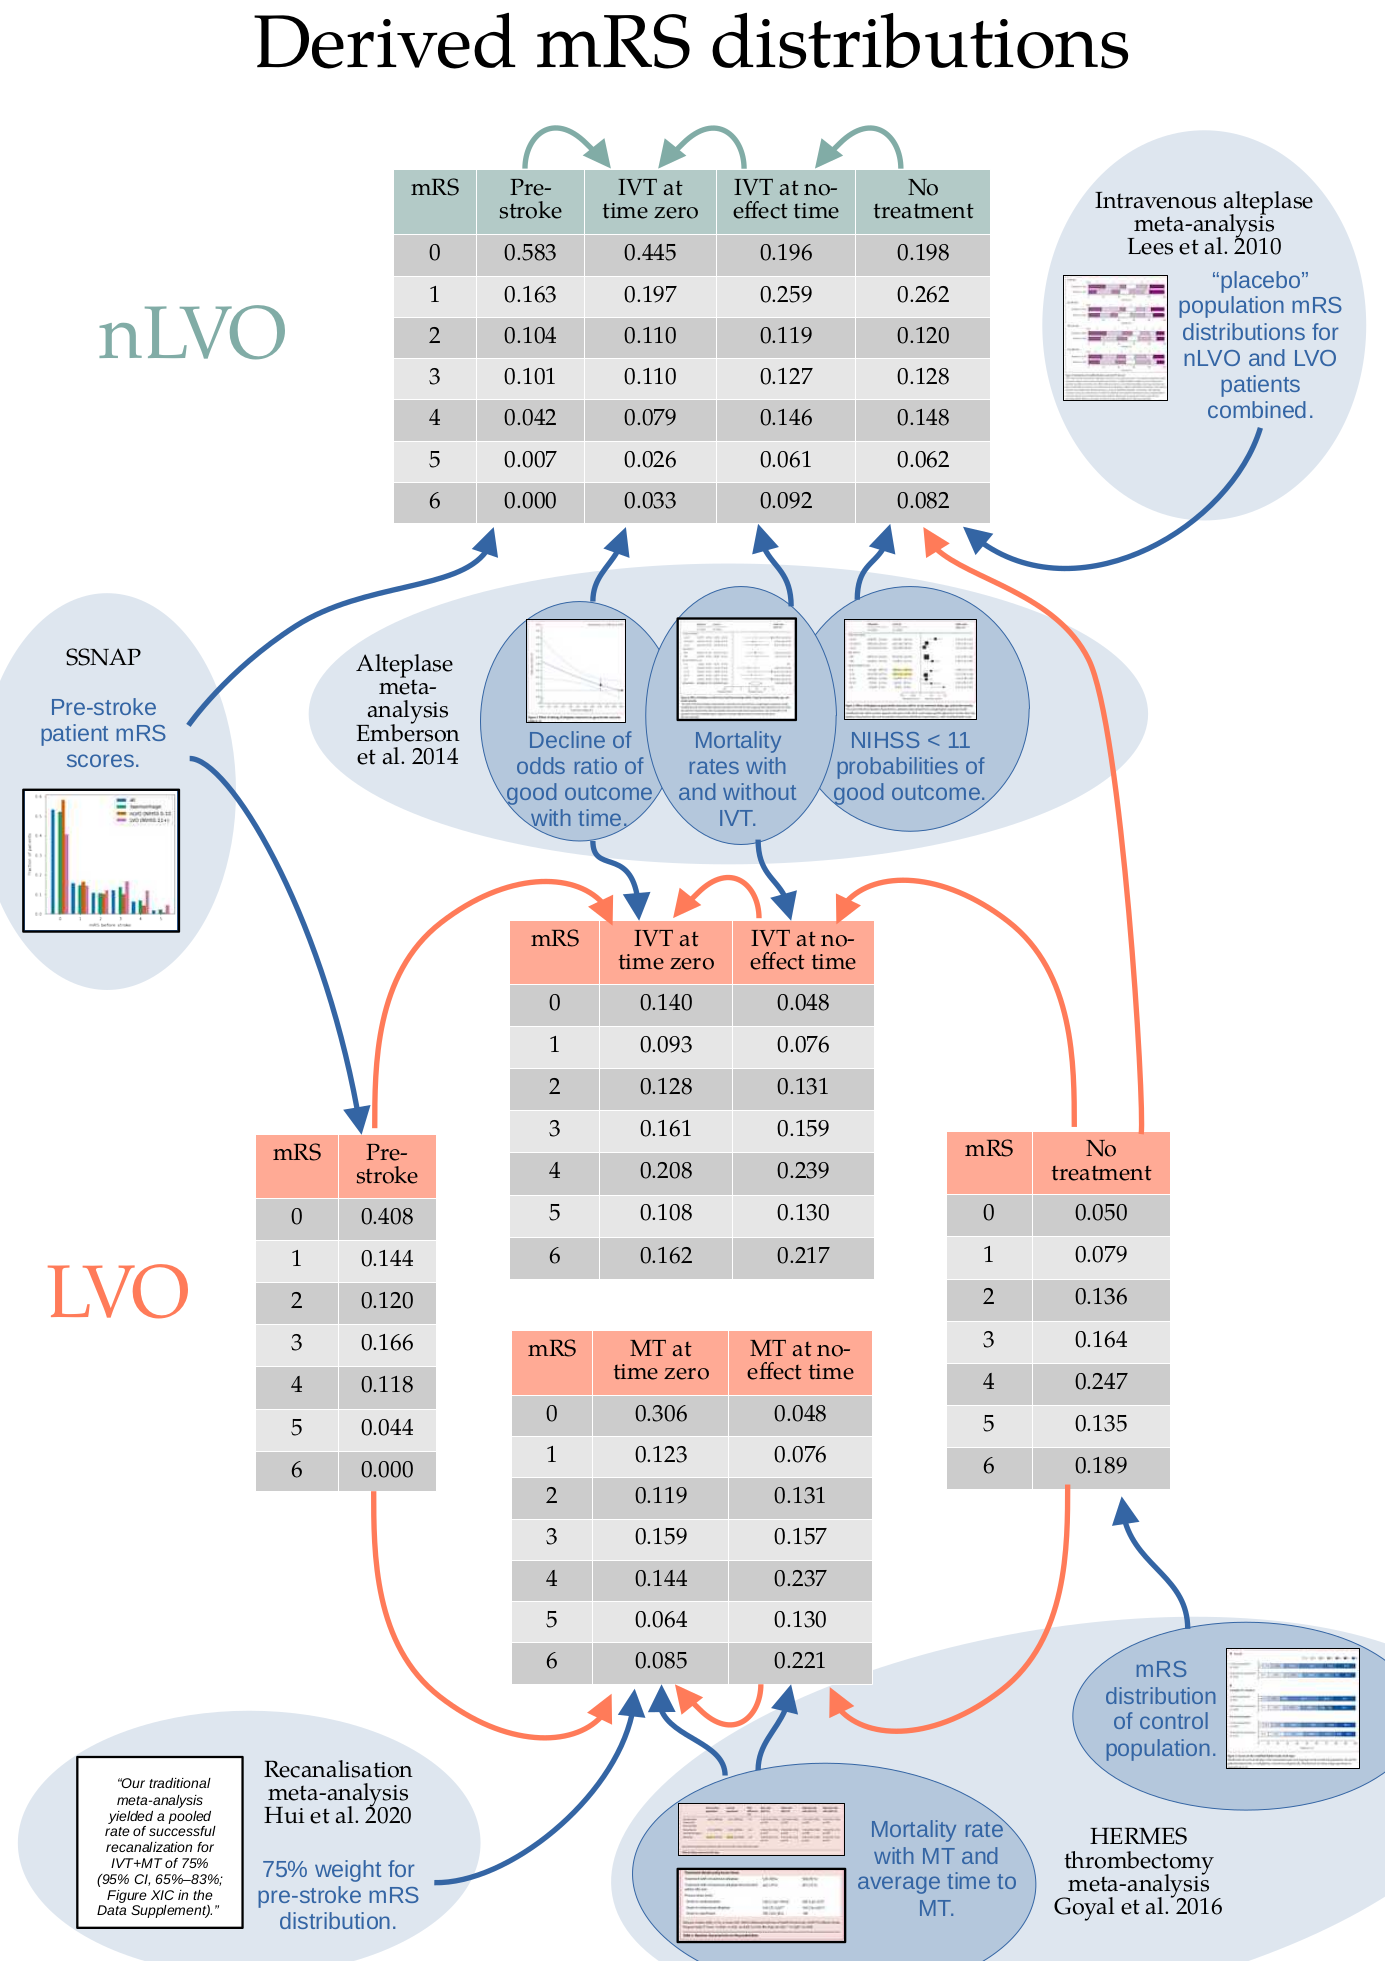
\includegraphics[width=1.0\linewidth]{images_modelling/data_sources_summary.png}
    \caption{Resulting reference distributions after combining data sources. Arrows show input and flow of data used to generate these populations.}
    \label{fig:data_sources_summary}
\end{figure}

\subsubsection{Pre-stroke mRS distributions}

The pre-stroke mRS distribution was from the national stroke audit for patients admitted to hospital with stroke between 2016 and 2018. A NIHSS of 0-10 was taken as a surrogate of LVO, and NIHSS 11+ as a surrogate of LVO. This cut-ff was found to have maximum discrimination between LVO and nLVO \cite{perez_de_la_ossa_effect_2022}. Resulting pre-stroke mRS distributions are shown in table \ref{tab:pre_stroke}

\begin{table}
\caption{Pre-stroke mRS distributions for nLVO and LVO}\label{tab:pre_stroke}
\centering

\begin{tabular}{l | l l l l l l l}
mRS & 0 & 1 & 2 & 3 & 4 & 5 & 6 \\
\hline
nLVO & 0.583 & 0.163 & 0.104 & 0.101 & 0.042 & 0.007 & 0 \\
LVO & 0.408 & 0.144 & 0.12 & 0.166 & 0.118 & 0.044 & 0 \\
\end{tabular}
\end{table}

\subsubsection{No treatment mRS distributions}

For LVO, the estimated post-stroke mRS distribution was taken from the control population of the HEMRES trial \cite{goyal_endovascular_2016}. Though the control group also included patients who had received thrombolysis, patients who had been successfully treated with thrombolysis would typically not have reached selection for trials on thrombectomy \cite{tsivgoulis_successful_2018}.


For nLVO, we take the control population from the thrombolysis clinical trials \cite{emberson_effect_2014}. The meta-analysis provides the mRS breakdown for control and treated groups (which will contain a mix of nLVO and LVO). The analysis also provides the proportion of patients mRS 0-1 for control and treated groups broken down into NIHSS subgroups. Those in the NIHSS 0-10 groups are assumed to be nLVO. The proportion mRS 0-1 in those subgroups is used to infer the full separate mRS distribution for patients in NIHSS 0-10 groups. 

Resulting pre-stroke mRS distributions are shown in table \ref{tab:no_treatment}. 

\begin{table}
\caption{No-treatment mRS distributions for nLVO and LVO}\label{tab:no_treatment}
\centering
\begin{tabular}{l | l l l l l l l}
mRS & 0 & 1 & 2 & 3 & 4 & 5 & 6 \\
\hline
nLVO & 0.198 & 0.262 & 0.120 & 0.128 & 0.148 & 0.062 & 0.082 \\
LVO & 0.050 & 0.079 & 0.136 & 0.164 & 0.247 & 0.135 & 0.189 \\
\end{tabular}
\end{table}

\subsubsection{Treatment at the no-effect time}

For treatment at the no-effect time, we expect the distribution to be the same as untreated, but with some treatment-related deaths.

For IVT, the meta-analysis of clinical trials \cite{emberson_effect_2014} reports deaths from intracranial haemorrhage. The IVT-related death rate is taken as the difference between treatment and control groups, split by NIHSS 0-10 (a surrogate for nLVO) and NIHSS 11+ (a surrogate for LVO).

For MT, treatment-related deaths must be inferred from available data. The steps were:

\begin{itemize}
    \item We identified a reference data point where both the death rate and time to treatment were known. We use the mean time to treatment and the mortality rate from the HERMES meta-analysis \cite{goyal_endovascular_2016}.
    \item Use pre-stroke population as a surrogate for 'full recanalisation', but assume only 75\% patients achieve recanalisation \cite{hui_efficacy_2020}.
    \item Assume that the beneficial effect of thrombectomy decays to zero in 6 hours \cite{fransen_time_2016}.
    \item Find the number of treatment-related deaths that would adjust the number of deaths at our given time point to the observed value. This figure is 4.0\%.
\end{itemize}

These steps are shown diagrammatically in figure \ref{fig:mt_deaths}.

Resulting estimates of treatment-related deaths are shown in table \ref{tab:treatment_deaths}.  

\begin{figure}[h!]
    \centering
    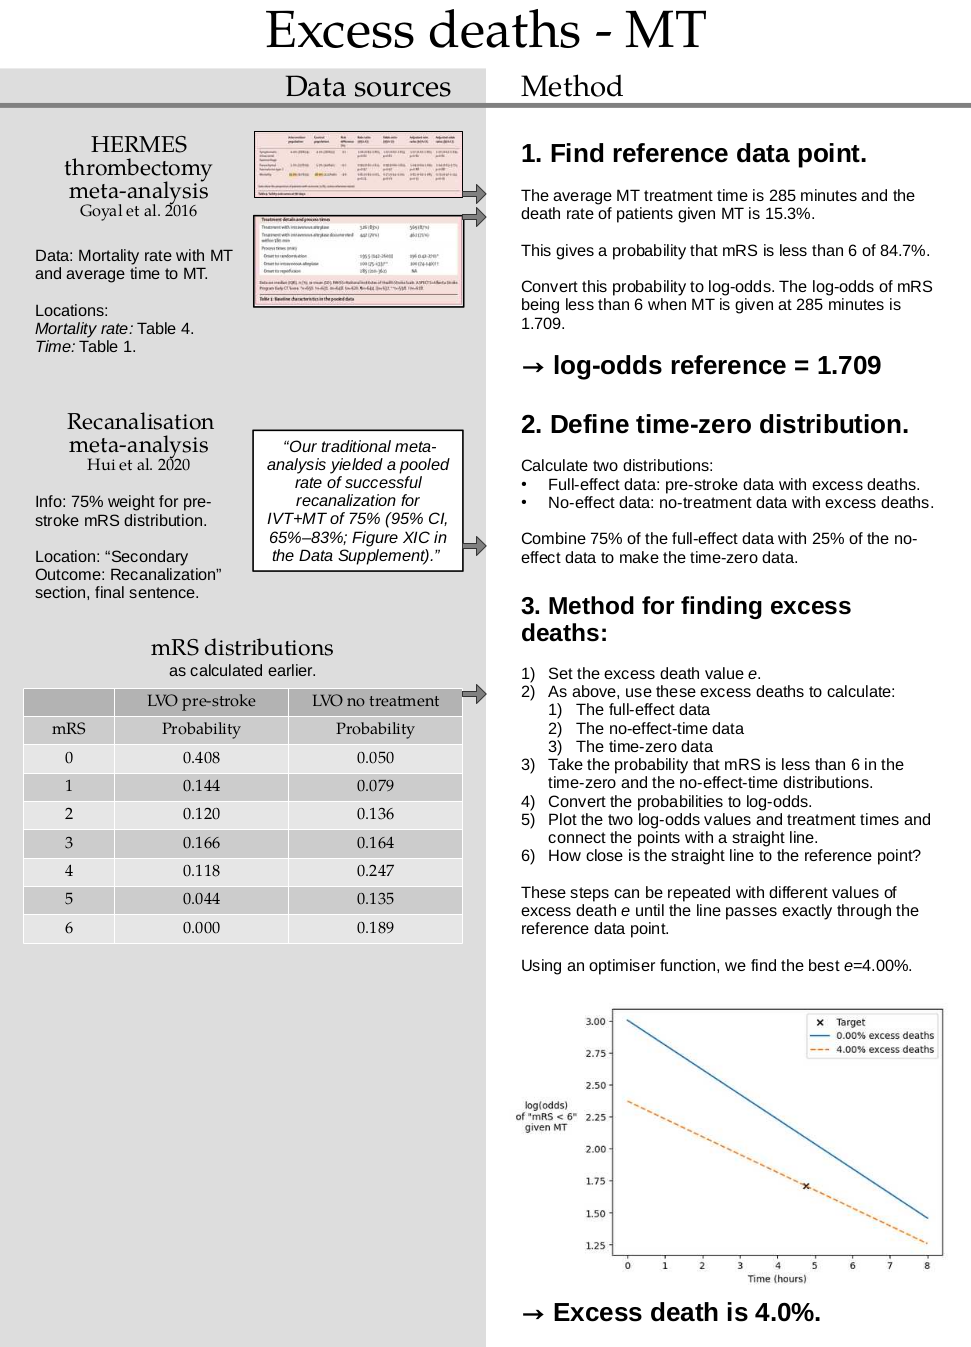
\includegraphics[width=1.0\linewidth]{images_modelling/data_sources_excess-death-mt.png}
    \caption{Overview of method to estimate treatment-related deaths for MT.}
    \label{fig:mt_deaths}
\end{figure}


\begin{table}[h!]
    \centering
    \caption{Estimated treatment-related deaths}
    \begin{tabular}{l l}
    Patient group & Treatment-related death rate\\
    \hline
    nLVO with IVT & \textbf{1.1\%}\\
    LVO with IVT & \textbf{3.4\%}\\
    LVO with MT & \textbf{4.0\%}\\
    \end{tabular}
    \label{tab:treatment_deaths}
\end{table}

\subsection{Interpolating effectiveness of treatment depending on time to treatment}

Once mRS distributions have been calculated for treatment given at time of stroke onset (time zero) and time of no-effectiveness of treatment, we interpolate between the two distributions based on a linear change in log-odds of reaching any given mRS threshold (which is the relationship used in clinical trials of thrombolysis and thrombectomy \cite{emberson_effect_2014, fransen_time_2016}). These may then be converted to odds, and then probability ($P = \frac{odds}{1 + odds}$).

We assumed that the time of no-effect was 6.3 hours after stroke onset for IVT \cite{emberson_effect_2014}, and 8.0 hours for MT \cite{fransen_time_2016}.

Figure \ref{fig:interpolation} shows interpolation of the effectiveness of treatment, using LVO treated with MT as an example.

\begin{figure}[h!]
    \centering
    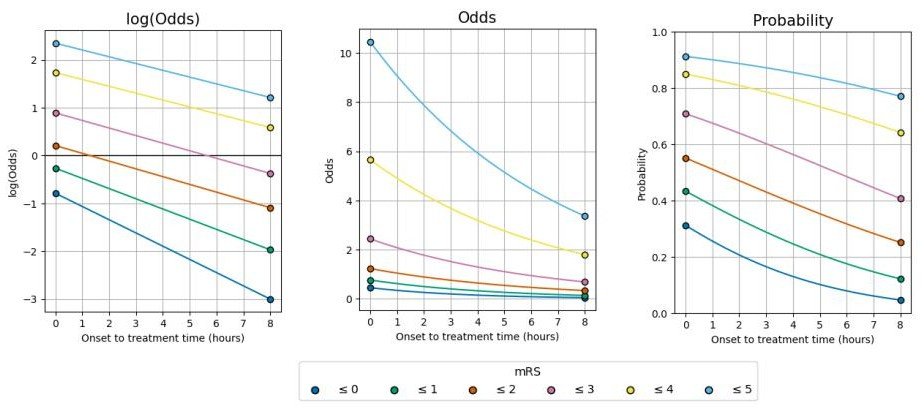
\includegraphics[width=1.0\linewidth]{images_modelling/log_odds_to_probs.jpg}
    \caption{Predicting outcomes based on interpolation between time of stroke onset and time of no-effect of treatment. This examples shows the effect of MT for patients with LVO stroke.}
    \label{fig:interpolation}
\end{figure}




%\section{Supplementary material}

\subsection{Outcome modelling}

We derived each mRS distribution for treatment at \emph{t=0} using the methodology of log-odds ratio of a good outcome falling linearly with time to treatment \cite{emberson_effect_2014, fransen_time_2016}. For each of the nLVO and LVO mRS distributions, we use the change of log-odds ratio of mRS 0-1 with time to IVT \cite{emberson_effect_2014} to scale the probability of mRS 0-1 from \emph{t=No Effect} to \emph{t=0}. We also require the mRS distributions for each patient cohort pre-stroke (sourced from SSNAP data) and if they received no treatment. The nLVO no-treatment population is the weighted difference of no-treatment populations containing both patients with nLVOs and LVOs \cite{lees_time_2010} and containing only LVO patients \cite{goyal_endovascular_2016}, where weights of 149\% and 49\% respectively result in the nLVO no-treatment probability of mRS 0-1 matching a reference population \cite{emberson_effect_2014}. The resulting proportions of LVO (49\%) and nLVO (51\%) patients are similar to those in clinical trials \cite{ist-3_collaborative_group_benefits_2012, emberson_effect_2014}. 
These \emph{t=0} mRS 0-1 data inform the weights for weighted averages of the pre-stroke and \emph{t=No Effect} mRS distributions that create the full \emph{t=0} mRS distributions (64.3\% and 35.7\% for nLVO, 25.5\% and 74.5\% for LVO respectively). The resulting \emph{t=No Effect} and \emph{t=0} mRS distributions for nLVO are consistent with the decline of chance of mRS 0-1 with time \cite{holodinsky_modeling_2018}. The MT \emph{t=0} mRS distribution is defined as the weighted average of 75\% of the pre-stroke and 25\% of the \emph{t=No Effect} distributions, following a reference rate of successful recanalisation \cite{hui_efficacy_2020}. The MT excess death rate is set to 4.0\% to ensure that log-odds falling linearly with time between the values of mRS 0-5 in the \emph{t=0} and in the \emph{t=No Effect} mRS distributions is consistent with a reference average mortality rate at the average MT time \cite{goyal_endovascular_2016}. The resulting \emph{t=0} and \emph{t=No Effect} mRS 0-2 probabilities give close matches to a reference decline of chance of mRS 0-2 with time \cite{fransen_time_2016}.

The time to no effect was 6.3 hours for IVT \cite{emberson_effect_2014} and 8.0 hours for MT \cite{ fransen_time_2016} (our model did not include selection of patients who may still benefit from treatment beyond these durations). We derived each \textit{No Effect} mRS distribution by applying the excess death rate due to treatment equally across the patient’s mRS distribution had they not received treatment (to represent that no benefit from treatment has been received as it was given too late, but the patient has been exposed to the risk from receiving the treatment).

We calculate the remaining IVT data using excess death rates of 1.1\% for nLVO and 3.4\% for LVO, from the difference in death rates of trial groups given IVT and given no treatment \cite{emberson_effect_2014}.

\subsection{Zoom in on benefit around one CSC (MSU base location)}

Figure \ref{fig:map_zoom} shows details of area of benefit/disbenefit of using MSU care over usual care. There is a halo of maximum benefit further out from the CSC where patients avoid an inter-hospital transfer (and associated delays for MT), but this enhanced benefit erodes with further travel time for the MSU.

\begin{figure}[h!]
    \centering
    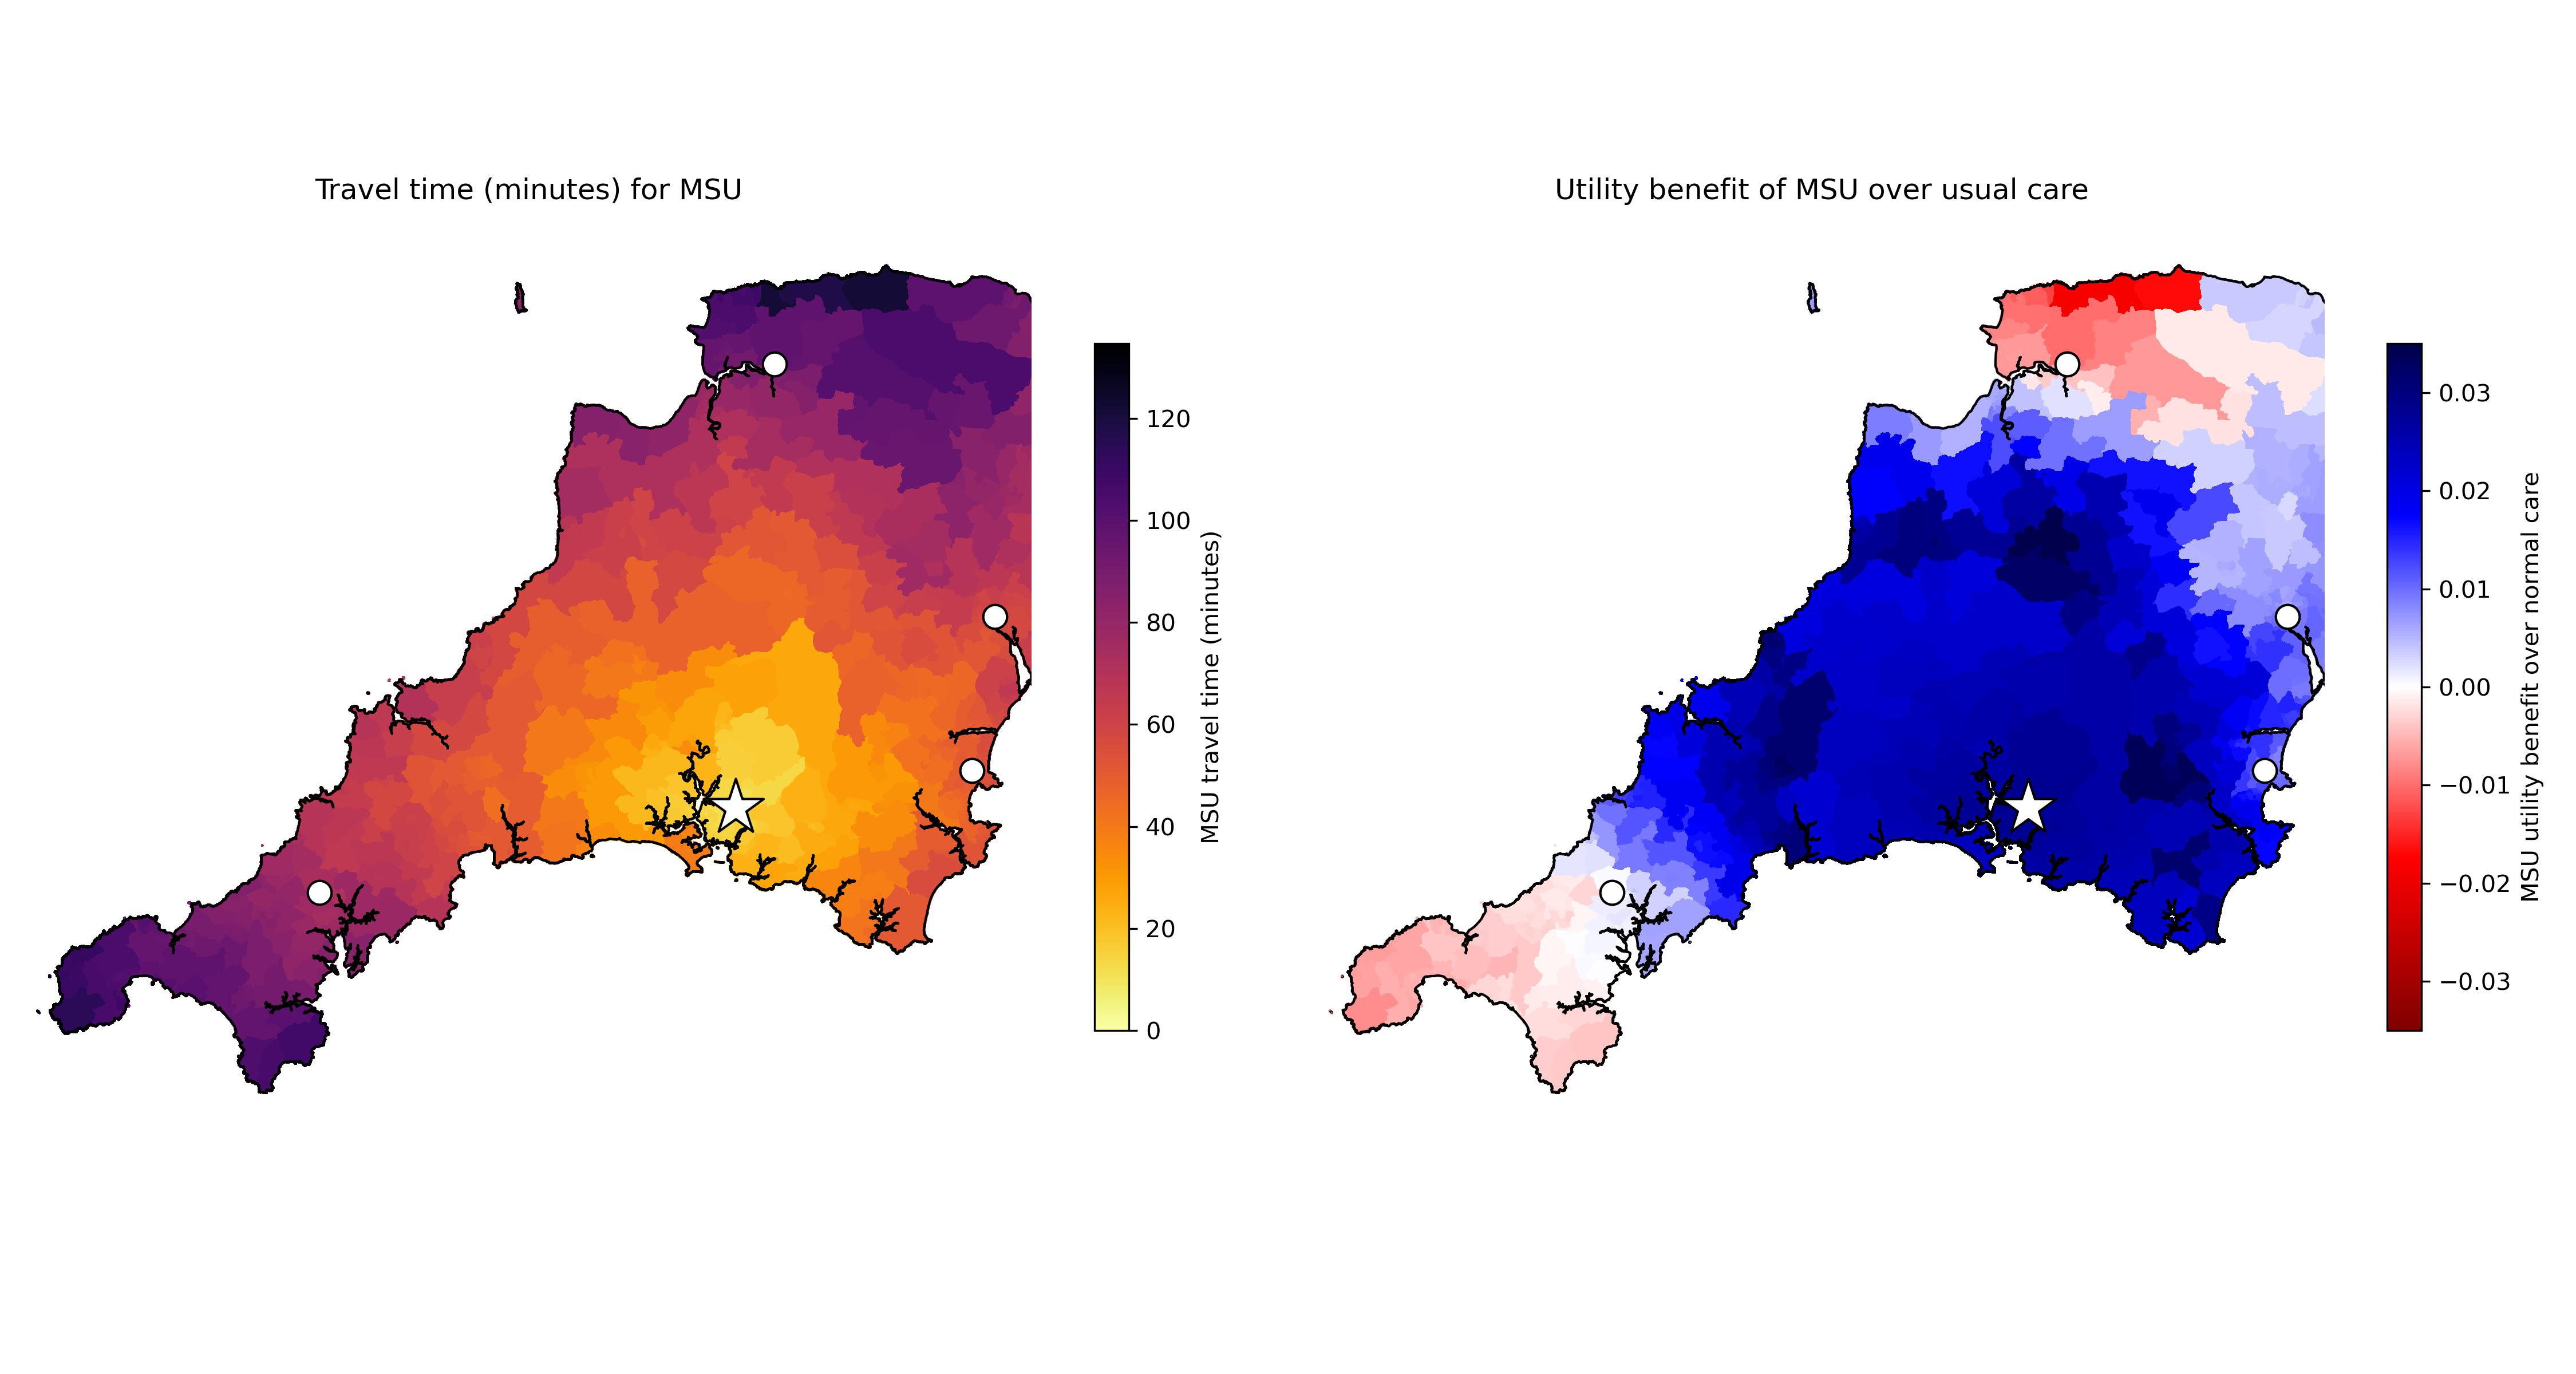
\includegraphics[width=1.0\linewidth]{images/map_zoom.jpg}
    \caption{Travel time for the MSU (to patient, and return travel for MT) and the utility benefit of using MSU care over usual care.}
    \label{fig:map_zoom}
\end{figure}

\subsection{Top 10 locations for MSUs}

Figure \ref{fig:top_10} shows the first 10 locations chosen by a greedy algorithm, where MSU locations are added one at a time, with each new location selected based on the best possible improvement in utility by adding one more unit.

\begin{figure}[h!]
    \centering
    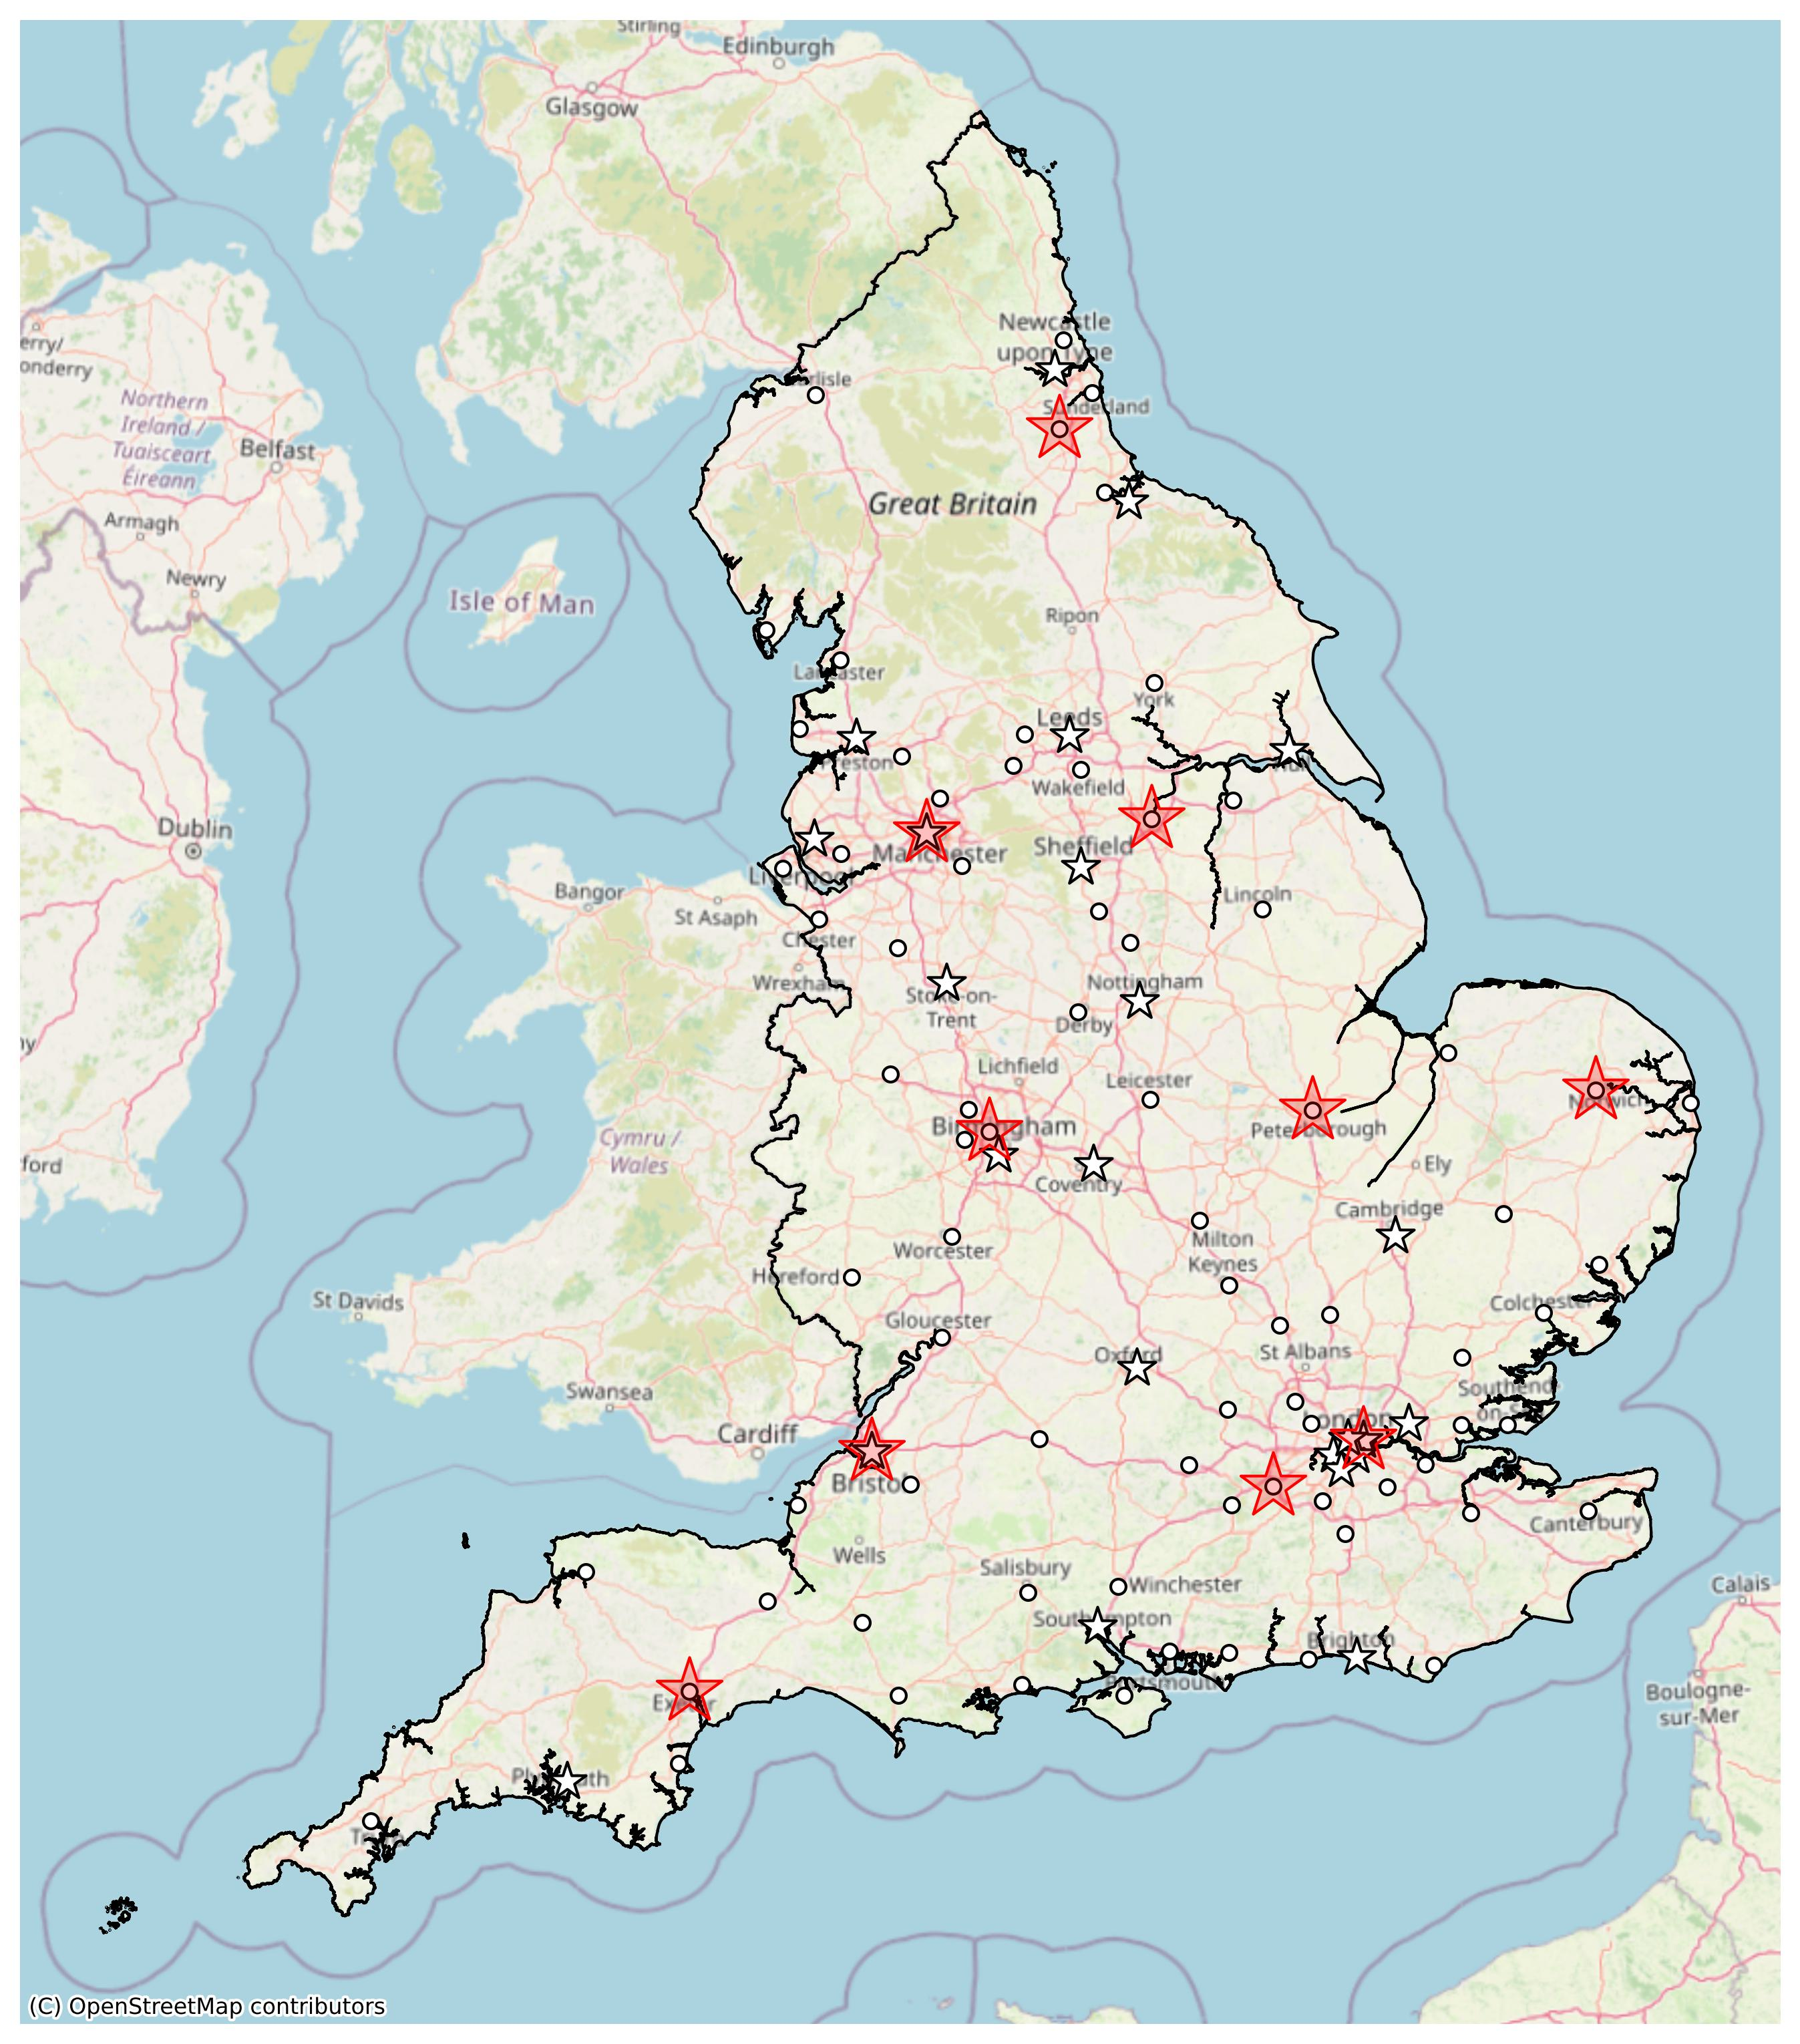
\includegraphics[width=1.0\linewidth]{images/top_10_msu_map.jpg}
    \caption{Top 10 locations (red stars) chosen by a greedy algorithm for maximising benefit from MSUs. White circles show locations of PSCs (providing only IVT). White stars show locations of CSCs.}
    \label{fig:top_10}
\end{figure}
\printbibliography[title={References for supplementary material}]
%TC:endignore
\end{refsection}


\end{document}